% \pdfoutput=1
\documentclass[11pt,a4paper]{article}

% --- FONTS & LANG ---
\usepackage{fontspec}
\defaultfontfeatures{Ligatures=TeX}
% \setmainfont{Times New Roman} % any Unicode font with Cyrillic works
\setmainfont{Libertinus Serif} 
% \setsansfont{Helvetica Neue}
% \setmonofont{Menlo}
\usepackage[main=english,russian]{babel}

% --- OTHER PACKAGES ---
\usepackage{geometry,setspace}
\geometry{margin=1in}
\onehalfspacing
\usepackage{amsmath,amssymb,amsfonts,amsthm}
\usepackage{natbib}
\usepackage{graphicx}
\usepackage{hyperref}
\usepackage{booktabs}
\usepackage{filecontents}
\usepackage{array}
\usepackage{enumitem}
\usepackage{tikz}
\usepackage{xcolor}
\usepackage{titlesec}
\usetikzlibrary{positioning,arrows.meta,fit,calc,shadows,backgrounds,shapes.geometric}
\hypersetup{unicode=true,colorlinks=true,linkcolor=blue,citecolor=blue,urlcolor=blue}


% \documentclass[11pt,a4paper]{article}

% % ==================== PACKAGES ====================
% \usepackage[utf8]{inputenc}
% \usepackage[T2A,T1]{fontenc}
% \usepackage[russian,english]{babel}
% \usepackage{lmodern}
% \usepackage{geometry}
% \geometry{margin=1in}
% \usepackage{setspace}
% \onehalfspacing
% \usepackage{amsmath,amssymb,amsthm,mathtools}
% \usepackage{graphicx}
% \usepackage{xcolor}
% \usepackage{hyperref}
% \usepackage{natbib}
% \usepackage{mdframed}
% \usepackage{booktabs}
% \usepackage{filecontents}
% \usepackage{enumitem}
% \usepackage{float}
% \usepackage{caption}
% \usepackage{subcaption}
% \usepackage{epigraph}
% \usepackage{tikz}
% \usetikzlibrary{shapes,arrows,positioning,decorations.pathreplacing}
% \usepackage{tabularx}
% \usepackage{wrapfig}

% ==================== CUSTOM COMMANDS ====================
\newcommand{\SYSTEM}{\textbf{SYSTEM}}
\newcommand{\SES}{\textbf{SES}}
\newcommand{\deltaDehum}{$\delta$-dehumanization}
\newcommand{\CC}{$\mathcal{C}$}
\newcommand{\CU}{$\mathcal{C}_U$}
\newcommand{\Fall}{\textit{Fall}}
\newcommand{\Love}{$\mathcal{L}$}
\newcommand{\LL}{$\mathcal{L}$}
\newcommand{\Suffering}{$\mathcal{S}$}
\newcommand{\SScri}{$\mathcal{S}$}
\newcommand{\SVE}{\textit{S.V.E.}}
\newcommand{\RR}{\mathbb{R}}
\newcommand{\EE}{\mathbf{E}}
\newcommand{\PEMY}{\textbf{PEMY}}

% ==================== COLORS ====================
\definecolor{sveblue}{RGB}{0, 51, 102}
\definecolor{sveteal}{RGB}{0, 102, 153}
\definecolor{svered}{RGB}{204, 0, 0}
\definecolor{sokratesblue}{RGB}{41, 128, 185}
\definecolor{solomongold}{RGB}{243, 156, 18}
\definecolor{ivangreen}{RGB}{39, 174, 96}
\definecolor{warningred}{RGB}{220, 20, 60}
\definecolor{hopegreen}{RGB}{46, 125, 50}

% ==================== HYPERREF SETUP ====================
\hypersetup{
    colorlinks=true,
    linkcolor=sveblue,
    citecolor=sveteal,
    urlcolor=sokratesblue,
    pdftitle={S.V.E. XII: THE SYSTEM — Diagnosis, Geometry of the Fall, and the Path to Collective Awareness},
    pdfauthor={Dr. Artiom Kovnatsky et al.}
}

% ==================== THEOREM ENVIRONMENTS ====================
\theoremstyle{definition}
\newtheorem{definition}{Definition}[section]
\newtheorem{axiom}{Axiom}[section]
\newtheorem{proposition}{Proposition}[section]
\newtheorem{parameter}{Parameter}[section]
\newtheorem{theorem}{Theorem}[section]
\newtheorem{corollary}{Corollary}[theorem]
\newtheorem{lemma}[theorem]{Lemma}
\theoremstyle{remark}
\newtheorem{remark}{Remark}[section]
\newtheorem{example}{Example}[section]
\newtheorem{insight}{Insight}[section]

% Custom environment for key insights
\newenvironment{keyinsight}[1]
{
    \begin{mdframed}[backgroundcolor=hopegreen!10,linecolor=hopegreen,linewidth=2pt]
    \textbf{Key Insight (#1):}
}
{
    \end{mdframed}
}

% Custom environment for warnings
\newenvironment{systemwarning}[1]
{
    \begin{mdframed}[backgroundcolor=warningred!10,linecolor=warningred,linewidth=2pt]
    \textbf{⚠ System Warning (#1):}
}
{
    \end{mdframed}
}

% ==================== BIBLIOGRAPHY ====================
\begin{filecontents*}{\jobname.bib}
@book{smith1776wealth,
  title={An Inquiry into the Nature and Causes of the Wealth of Nations},
  author={Smith, Adam},
  year={1776},
  publisher={W. Strahan and T. Cadell}
}
@article{dzendialogue,
    title={\foreignlanguage{russian}{Дзен-студия | Тренинг-Статья: Семена или Капитализм 2.0}},
    author={Kovnatsky, Artiom},
    year={2025},
    note={Training Article on Capitalism 2.0 and PEMY model}
}
@misc{spe1973,
    author = {Haney, C. and Banks, W. C. and Zimbardo, P. G.},
    year = {1973},
    title = {A study of prisoners and guards in a simulated prison},
    howpublished = {Naval Research Reviews, 9, 1--17}
}
@book{jung1969collective,
    author = {Jung, Carl G.},
    title = {The Archetypes and the Collective Unconscious},
    series = {Collected Works Vol. 9 Part 1},
    year = {1969},
    publisher = {Princeton University Press}
}
@book{plato_republic,
    author = {Plato},
    title = {The Republic},
    year = {380 BCE}
}
@misc{einsteinquote,
    author={Einstein, Albert},
    note={On spiritual evolution and rational knowledge}
}
@book{pereslegin2005summa,
    author = {Pereslegin, Sergey B.},
    title = {\foreignlanguage{russian}{Сумма стратегии}},
    year = {2005},
    publisher = {AST}
}
@book{machiavelli1532prince,
    author = {Machiavelli, Niccolò},
    title = {The Prince},
    year = {1532}
}
@book{suntzu_artofwar,
    author = {Sun Tzu},
    title = {The Art of War},
    year = {5th century BCE}
}
@misc{russell_education,
    author = {Russell, Bertrand},
    title = {On Education},
    note = {Nobel Prize in Literature, 1950}
}
@misc{brettonwoods1971,
    title={The End of the Bretton Woods System and the Nixon Shock},
    year={1971}
}
@misc{tuskegee,
    title = {Tuskegee Syphilis Study},
    year = {1932--1972}
}
@misc{guatemala_syphilis,
    title = {Guatemala Syphilis Experiments},
    year = {1946--1948}
}
@misc{operation_paperclip,
    title = {Operation Paperclip},
    year = {1945--1959}
}
@misc{sve0,
    author = {Kovnatsky, Artiom},
    title = {S.V.E. 0: SIP and EBP Protocols},
    year = {2024}
}
@misc{sve4,
    author = {Kovnatsky, Artiom},
    title = {S.V.E. IV: Christ-Vector and Geodesic Ethics},
    year = {2024}
}
@misc{sve8,
    author = {Kovnatsky, Artiom},
    title = {S.V.E. VIII: Divine Mathematics - Mathematical Foundations},
    year = {2024}
}
@misc{sve9,
    author = {Kovnatsky, Artiom},
    title = {S.V.E. IX: Verification and Falsification},
    year = {2024}
}
@misc{sve10,
    author = {Kovnatsky, Artiom},
    title = {S.V.E. X: Cognitive Operating System},
    year = {2024}
}
@misc{sve11,
    author = {Kovnatsky, Artiom},
    title = {S.V.E. XI: Practical Philosophy and Personal Transformation},
    year = {2024}
}
@book{piketty2014capital,
    author = {Piketty, Thomas},
    title = {Capital in the Twenty-First Century},
    year = {2014},
    publisher = {Harvard University Press}
}
@book{taleb2012antifragile,
    author = {Taleb, Nassim Nicholas},
    title = {Antifragile: Things That Gain from Disorder},
    year = {2012},
    publisher = {Random House}
}
@book{kahneman2011thinking,
    author = {Kahneman, Daniel},
    title = {Thinking, Fast and Slow},
    year = {2011},
    publisher = {Farrar, Straus and Giroux}
}
\end{filecontents*}

% ==================== DOCUMENT ====================
\begin{document}

% ==================== TITLE PAGE ====================
\begin{titlepage}
    \centering
    \vspace*{2cm}
    
    {\Huge\bfseries S.V.E. XII: THE SYSTEM\\[0.5cm]}
    {\LARGE\textcolor{sveblue}{Diagnosis, Geometry of the Fall,\\and the Path to Collective Awareness}}
    
    \vspace{2cm}
    
    \begin{figure}[H]
        \centering
        \includegraphics[width=0.7\textwidth]{fig/main_illustration_invisible_hand_subconciousness.png}
        \caption*{The Invisible Hand and the Architecture of Subconsciousness}
    \end{figure}
    
    \vspace{1cm}
    
    {\Large Dr. Artiom Kovnatsky \textit{et al.}}
    
    \vspace{1cm}
    
    {\large S.V.E. Series XII\\
    Integrating Philosophy, Mathematics, and Systems Science}
    
    \vfill
    
    \date{Draft v0.9 — October 26, 2025\\\small (Work in progress — feedback welcome)}
    
\end{titlepage}

% ==================== ABSTRACT ====================
\begin{abstract}
\noindent
This paper presents a comprehensive diagnosis of humanity's current socio-economic-spiritual crisis through the lens of \SVE{} (Spiritual Values Evolution) theory. We introduce \textbf{SYSTEM}---a self-reinforcing pattern of collective unconsciousness that drives humanity toward increasing inequality, dehumanization, and suffering---and provide both mathematical formalization and practical solutions.

\vspace{0.5em}

\textbf{Key contributions:}
\begin{itemize}[leftmargin=*]
    \item Formalization of Socio-Economic-Spiritual State (\SES{}) as a multi-dimensional manifold
    \item Mathematical modeling of \deltaDehum{} dynamics and self-reinforcing deterioration cycles
    \item Geometric interpretation of humanity's ``Fall'' in consciousness space
    \item Introduction of PEMY (People + Environment + Money + You) as a practical alternative to extractive capitalism
    \item Integration of consciousness theory, economics, and systems science into a unified framework
    \item Actionable pathways for individual and collective transformation
\end{itemize}

\vspace{0.5em}

We argue that current crises (inequality, environmental collapse, meaning crisis) are not separate problems but symptoms of a single underlying pattern: humanity's disconnection from consciousness-guided action. The paper provides both diagnostic tools and therapeutic interventions, grounded in falsifiable predictions and empirical verification protocols.

\vspace{0.5em}

\textit{Keywords:} consciousness theory, socio-economic systems, inequality dynamics, spiritual evolution, PEMY model, collective unconsciousness, systems transformation, geodesic ethics
\end{abstract}

% --- SVE PUBLIC LICENSE v1.0 NOTICE ---
\vspace{1em} % Adjust spacing as needed
\begin{center}
\begin{minipage}{0.85\textwidth} % Adjust width as needed
\centering
\itshape\small % Italic and small font size
This work is licensed under the SVE Public License v1.0 (based on CC BY-NC-SA 4.0 with a mandatory SVE Addendum).
Full license text is available at: \\
\href{https://www.artiomkovnatsky.com/posts/license/}{artiomkovnatsky/license} (Web version) \\
\href{https://github.com/skovnats/psite/blob/master/static/licenses/SVE_Public_License_v1.0.pdf}{GitHub Repository} (Canonical PDF/LaTeX source)
\end{minipage}
\end{center}
\vspace{1em} % Adjust spacing as needed
% --- END SVE PUBLIC LICENSE v1.0 NOTICE ---

\newpage


% ==================== TABLE OF CONTENTS ====================
\clearpage
\tableofcontents
\clearpage
\setcounter{page}{1}


% ========================= S.V.E. Universe Navigation (FINAL) =========================
% Place after Abstract
\clearpage
\thispagestyle{empty}

% Define colors if not already defined
\providecolor{sveblue}{RGB}{0, 51, 102}
\providecolor{sveteal}{RGB}{0, 102, 153}

\begin{center}
\vspace*{1cm}

{\fontsize{16}{20}\selectfont\textbf{\textcolor{sveblue}{The S.V.E. Universe}}}

\vspace{0.3em}
{\large\textcolor{sveteal}{Systemic Verification Engineering | Navigation Map}}

\vspace{0.5em}
\hrule height 1pt
\vspace{1.2em}

% ----------------------------- Conceptual map ---------------------------------
\begin{tikzpicture}[
    node distance=1.2cm,
    every node/.style={align=center, font=\small},
    foundation/.style={rectangle, draw=sveblue, thick, fill=sveblue!5, rounded corners, minimum width=3.6cm, minimum height=0.9cm},
    engine/.style={rectangle, draw=orange!70!black, thick, fill=orange!10, rounded corners, minimum width=3.6cm, minimum height=0.9cm},
    application/.style={rectangle, draw=sveteal, thick, fill=sveteal!5, rounded corners, minimum width=3.6cm, minimum height=0.9cm},
    synthesis/.style={rectangle, draw=sveblue, thick, fill=purple!10, rounded corners, minimum width=3.6cm, minimum height=0.9cm},
    arrow/.style={->, >=latex, thick, color=sveblue!70}
]

% Foundation layer (0–II)
\node[foundation] (ebp) {\textbf{0 (1): EBP}\\Epistemological Boxing};
\node[foundation, right=0.6cm of ebp] (sip) {\textbf{0 (2): SIP}\\Computational Truth};
\node[foundation, right=0.6cm of sip] (theorem) {\textbf{I: Theorem}\\Systemic Diagnosis};
\node[foundation, right=0.6cm of theorem] (arch) {\textbf{II: Architecture}\\3-Stage Solution};

% Engine layer (new: X–XI)
\node[engine, below=1.4cm of ebp, xshift=1.9cm] (triple) {\textbf{X: Triple Architect CogOS}\\Socrates | Solomon | Ivan};
\node[engine, right=0.6cm of triple] (vkb) {\textbf{XI: Verifiable KB / Distributed IVM}\\Knowledge DAG + DAO};

% Application layer (III–VI)
\node[application, below=1.5cm of triple, xshift=-1.9cm] (science) {\textbf{III: Science}\\Academic Integrity};
\node[application, right=0.6cm of science] (ethics) {\textbf{IV: Ethics}\\Beacon Protocol};
\node[application, right=0.6cm of ethics] (democracy) {\textbf{V: Democracy}\\Governance OS};
\node[application, right=0.6cm of democracy] (security) {\textbf{VI: Security}\\Cognitive Sovereignty};

% More applications & models (VII) and synthesis (VIII–IX, XII)
\node[application, below=1.5cm of science] (models) {\textbf{VII: Models}\\Hybrid Structures};
\node[synthesis, below=1.5cm of ethics] (divine) {\textbf{VIII: Divine Math}\\Unified Theory};
\node[synthesis, below=1.5cm of democracy] (integrated) {\textbf{IX: Integration}\\Complete Framework};
\node[synthesis, below=1.5cm of security] (system) {\textbf{XII: SYSTEM}\\Diagnosis \& Response-Path};

% Directed flow
\draw[arrow] (ebp) -- (triple);
\draw[arrow] (sip) -- (triple);
\draw[arrow] (theorem) -- (vkb);
\draw[arrow] (arch) -- (vkb);

\draw[arrow] (triple) -- (science);
\draw[arrow] (triple) -- (ethics);
\draw[arrow] (vkb) -- (democracy);
\draw[arrow] (vkb) -- (security);

\draw[arrow] (science) -- (models);
\draw[arrow] (ethics) -- (divine);
\draw[arrow] (democracy) -- (integrated);
\draw[arrow] (security) -- (system);

% Cross-links (dashed)
\draw[arrow, dashed] (models) to[bend right=10] (divine);
\draw[arrow, dashed] (divine) -- (integrated);
\draw[arrow, dashed] (integrated) -- (system);
\draw[arrow, dashed] (ebp) to[bend right=12] (sip);
\draw[arrow, dashed] (sip) to[bend right=12] (theorem);
\draw[arrow, dashed] (theorem) to[bend right=12] (arch);

\end{tikzpicture}

\vspace{1.2em}
\hrule height 0.5pt
\vspace{0.8em}
\end{center}

% --------------------------------- Descriptions ---------------------------------
\begin{small}
\subsection*{\textcolor{sveblue}{Foundation | Theoretical Core}}
\begin{description}[leftmargin=1cm, style=nextline, itemsep=0.45em]
    \item[\textbf{S.V.E. 0 (1): The Epistemological Boxing Protocol}] 
    Structured, adversarial verification (\emph{cognitive gymnasium}) for stress-testing theses and synthesizing higher truth.

    \item[\textbf{S.V.E. 0 (2): The Socratic Investigative Process (SIP)}] 
    Computational truth-approximation via iterative vector purification, Meta-Verdict / Meta-SIP for complex analysis.

    \item[\textbf{S.V.E. I: The Theorem of Systemic Failure}] 
    \emph{Disaster Prevention Theorem}: without an independent verification mechanism (IVM), collective intelligence degrades.

    \item[\textbf{S.V.E. II: The Architecture of Verifiable Truth}] 
    Three-stage architecture ``Caesar vs God'': facts separated from values; antifragile design.
\end{description}

\subsection*{\textcolor{orange!70!black}{Engine | Operational Layer (NEW)}}
\begin{description}[leftmargin=1cm, style=nextline, itemsep=0.45em]
    \item[\textbf{S.V.E. X: Triple Architect CogOS}] 
    Cognitive OS for LLM: \textit{Socrates} (logic/falsification), \textit{Solomon} (ethics/wisdom), \textit{Ivan} (humility/empathy); 5 core rules (humility, Bayesian priors, 5-column verification, double Socratic ``tails'' 1+1>2, growth vector).

    \item[\textbf{S.V.E. XI: Verifiable Knowledge Base \& Distributed IVM}] 
    Verifiable Knowledge Base (DAG of SIP/Meta-SIP nodes) + DAO-managed context (PM.txt/VP.txt); three verification stages: SIP→EBP→peer-review; applications: StackOverflow 2.0, Wikipedia Reformation, Global Fact-Checking.
\end{description}

\subsection*{\textcolor{sveteal}{Applications | Domain Solutions}}
\begin{description}[leftmargin=1cm, style=nextline, itemsep=0.45em]
    \item[\textbf{S.V.E. III: The Protocol for Academic Integrity}] 
    SYSTEM-PURGATORY: transparent ``boxing match'' to combat replication crisis.
    \item[\textbf{S.V.E. IV: The Beacon Protocol}] 
    Geodesic ethics (manifold, ``Christ-vector'') for navigating radical uncertainty.
    \item[\textbf{S.V.E. V: OS for Verifiable Democracy}] 
    Fakten-TUV, Socrates Bot, operating system for institutional integrity.
    \item[\textbf{S.V.E. VI: Protocol for Cognitive Sovereignty}] 
    Cognitive sovereignty protocol: protection against groupthink and information warfare.
    \item[\textbf{S.V.E. VII: Hybrid Models of State Structure}] 
    Hybrid models (hierarchy + ``ant colony'') for antifragile governance.
\end{description}

\subsection*{\textcolor{sveblue}{Synthesis | Unified Framework}}
\begin{description}[leftmargin=1cm, style=nextline, itemsep=0.45em]
    \item[\textbf{S.V.E. VIII: Divine Mathematics}] 
    Unified theory of consciousness (geometry $\mathcal{A}\pi-\pi\Omega$), unification of ethics/economics/meaning.
    \item[\textbf{S.V.E. IX: Integrated SVE}] 
    Integration of Divine Math, Beacon Protocol and DPT (IVM) into unified framework.
    \item[\textbf{S.V.E. XII: THE SYSTEM}] 
    Diagnosis of collective dynamics (A1–A3; $\delta$-dehumanization; parametrization SES/P1–P5), ``Geometry of the Fall'', S.V.E. response (PEMY, CogOS X, VKB XI).
\end{description}

\vspace{0.6em}
\begin{center}
\small \textbf{\textit{Forthcoming Meta-SIP Applications (Series):}}
\vspace{0.3em}

\begin{minipage}{0.88\textwidth}
\begin{itemize}[nosep, itemsep=0.2em, topsep=0pt, leftmargin=1.5em]
    \item Geopolitical analysis \& conflict resolution
    \item National security \& intelligence assessment
    \item Policy verification \& legislative impact analysis
    \item Financial system stability \& economic forecasting
    \item AI safety \& alignment verification
    \item Climate policy \& complex systems modeling
    \item Public health \& scientific integrity assurance
    \item Addressing systemic disinformation \& cognitive security
\end{itemize}
\end{minipage}
\end{center}
\end{small}

\clearpage
% ======================= End S.V.E. Universe Navigation (FINAL) =======================

% ==================== EPIGRAPH ====================
\begin{figure}[H]
    \centering
    \includegraphics[width=0.5\textwidth]{fig/einstein_quote.png}
    \caption*{Einstein on spiritual evolution}
\end{figure}

\epigraph{
\foreignlanguage{russian}{``Проблема не может быть решена на том же уровне сознания, на котором она возникла.''}\\[0.3cm]
``A problem cannot be solved at the same level of consciousness that created it.''
}{--- Albert Einstein}

\vspace{1cm}

\epigraph{
``The line separating good and evil passes not through states, nor between classes, nor between political parties either---but right through every human heart.''
}{--- Aleksandr Solzhenitsyn}

% ==================== INTRODUCTION ====================
\section{Introduction: The Crisis of Our Time}

We live in an age of profound paradox. Humanity possesses unprecedented technological capability, scientific knowledge, and productive capacity---yet faces existential threats on multiple fronts: ecological collapse, extreme inequality, erosion of meaning, and the rise of systems that increasingly treat humans as resources rather than conscious beings.

\begin{figure}[H]
    \centering
    \includegraphics[width=0.85\textwidth]{fig/where_humanity_goes.png}
    \caption{Where is humanity heading? The diverging paths of conscious evolution and unconscious deterioration}
    \label{fig:humanity_trajectory}
\end{figure}

This is not merely a collection of separate problems to be solved individually. Rather, these crises are \textbf{symptoms of a single underlying pattern}---a self-reinforcing system that we call \textbf{SYSTEM}. This pattern operates primarily through \textit{unconscious} mechanisms: unexamined assumptions, inherited mental models, and automated behavioral scripts that persist across generations.

Think of SYSTEM like a computer operating system running in the background of collective human behavior---except instead of optimizing for user wellbeing, it optimizes for its own perpetuation, often at the expense of human consciousness, connection, and flourishing.

\subsection{The Invisible Architecture}

Adam Smith famously invoked the metaphor of the ``invisible hand'' of markets coordinating individual self-interest toward collective benefit. But what if there exists an \textit{invisible architecture} of unconscious patterns that coordinates individual actions toward collective harm?

\begin{figure}[H]
    \centering
    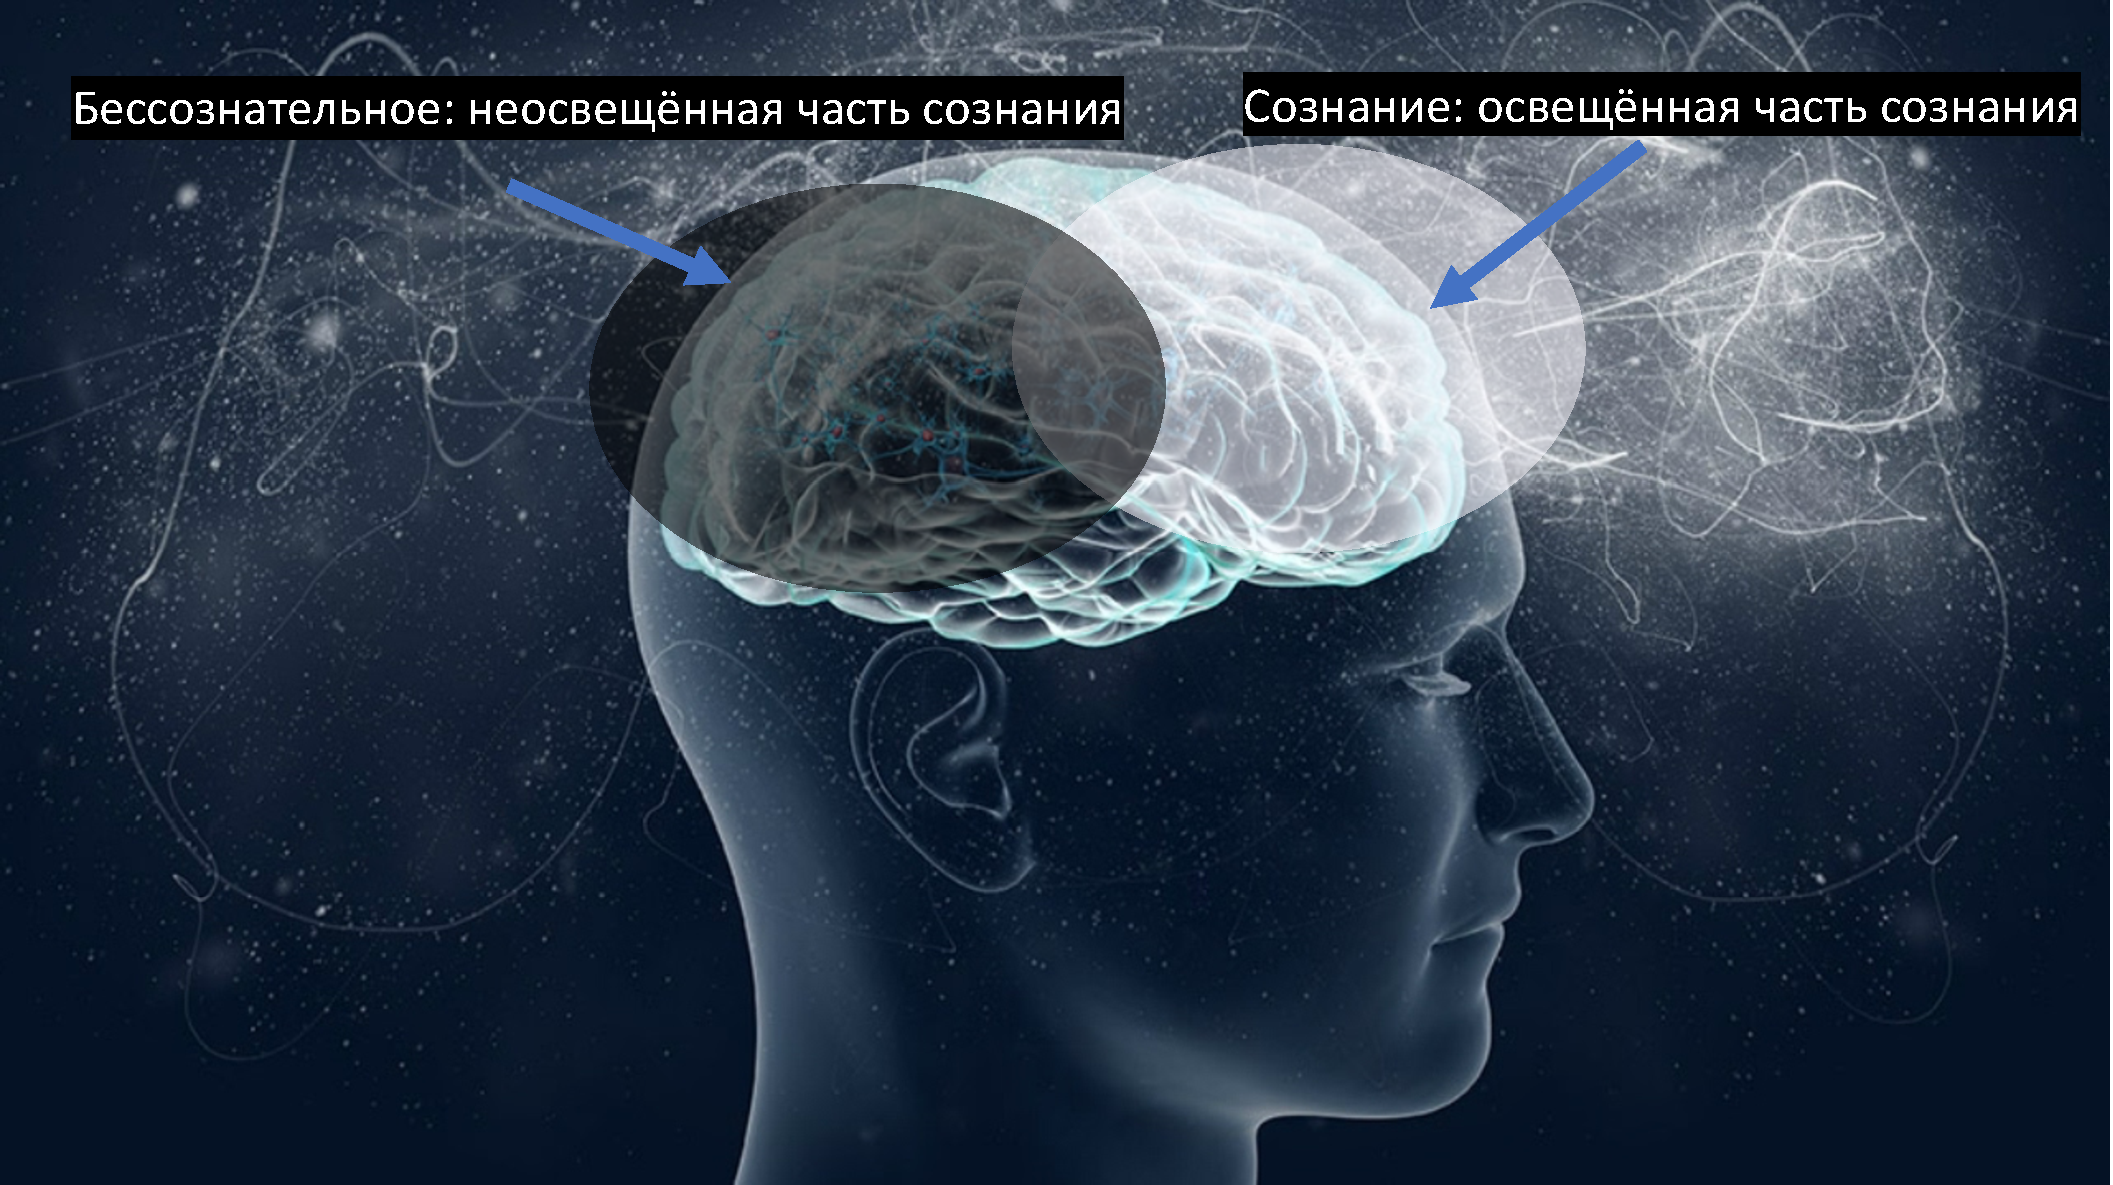
\includegraphics[width=0.8\textwidth]{fig/model_conciousness_subconsiousness.pdf}
    \caption{The architecture of consciousness and subconsciousness: how SYSTEM operates beneath awareness}
    \label{fig:consciousness_model}
\end{figure}

This paper makes that architecture visible. We will:

\begin{enumerate}
    \item \textbf{Diagnose} SYSTEM: identify its structure, dynamics, and self-reinforcing mechanisms
    \item \textbf{Formalize} its mathematics: provide rigorous models of how it evolves and propagates
    \item \textbf{Trace} its historical development: show how we arrived at this state
    \item \textbf{Prescribe} solutions: offer both individual practices and systemic alternatives
    \item \textbf{Provide verification protocols}: make our claims falsifiable and testable
\end{enumerate}

\subsection{Why This Matters Now}

We are at an inflection point. The trajectories of technological power, environmental degradation, and social fragmentation suggest that humanity has perhaps 20-50 years to fundamentally shift course. Not through incremental policy adjustments, but through a \textit{phase transition} in collective consciousness.

\begin{systemwarning}{Urgency Without Panic}
The urgency is real, but panic is counterproductive. SYSTEM thrives on fear, reactivity, and short-term thinking. Our response must be grounded, conscious, and strategic. This paper aims to catalyze clarity, not anxiety.
\end{systemwarning}

The good news: such transitions have happened before in human history. The shift from tribal to agricultural societies. The emergence of scientific thinking. The abolition of slavery. The expansion of human rights. Each represented a fundamental reorganization of consciousness and social structure.

We stand at the threshold of another such transition. But unlike previous shifts that happened gradually and unconsciously, this one must be \textit{conscious and intentional}. We must become the authors of our own evolution.

\subsection{Roadmap of This Paper}

\textbf{Part I (Sections 2-4):} \textit{Understanding SYSTEM}
\begin{itemize}
    \item Formal definition of Socio-Economic-Spiritual State (\SES)
    \item Mathematical models of \deltaDehum{} and feedback loops
    \item Historical analysis of how we got here
\end{itemize}

\textbf{Part II (Sections 5-7):} \textit{The Geometry of the Fall}
\begin{itemize}
    \item Consciousness manifold and geodesic paths
    \item Measurement and tracking of societal state
    \item Case studies and empirical evidence
\end{itemize}

\textbf{Part III (Sections 8-10):} \textit{Solutions and Transformation}
\begin{itemize}
    \item Individual practices for consciousness development
    \item PEMY model as systemic alternative
    \item Transition strategies and implementation
\end{itemize}

\textbf{Part IV (Sections 11-12):} \textit{Verification and Next Steps}
\begin{itemize}
    \item Falsifiable predictions
    \item Counterarguments and responses
    \item Practical action steps
\end{itemize}

\subsection{How to Read This Paper}

This work synthesizes philosophy, mathematics, psychology, economics, and systems theory. Not all readers will resonate with all sections equally. We suggest:

\begin{itemize}
    \item \textbf{Practically oriented readers:} Focus on Sections 1, 8-10, and 12
    \item \textbf{Theoretically oriented readers:} Don't skip the mathematical formalizations in Sections 3-6
    \item \textbf{Skeptical readers:} Jump to Section 11 for falsification criteria and counterarguments
    \item \textbf{All readers:} Pay attention to the figures---they often convey key insights more clearly than text
\end{itemize}

And remember: \textit{the map is not the territory}. These models are tools for understanding, not ultimate truths. Hold them lightly, test them against reality, and discard what doesn't serve.

\begin{keyinsight}{Reading Strategy}
If you find yourself resisting or emotionally reacting to certain sections, that's valuable data. SYSTEM often protects itself through emotional reactions to ideas that threaten its structure. Notice the resistance, examine it, and then engage with the content consciously.
\end{keyinsight}

% ==================== PART I: UNDERSTANDING SYSTEM ====================
\part{Understanding SYSTEM: Diagnosis of the Current State}

\section{Socio-Economic-Spiritual State (SES): Formal Definition}

Before we can diagnose SYSTEM, we need a framework for describing the state of human societies. We introduce the concept of \textbf{Socio-Economic-Spiritual State} (\SES)---a multi-dimensional representation of a society's condition across all relevant domains.

\begin{figure}[H]
    \centering
    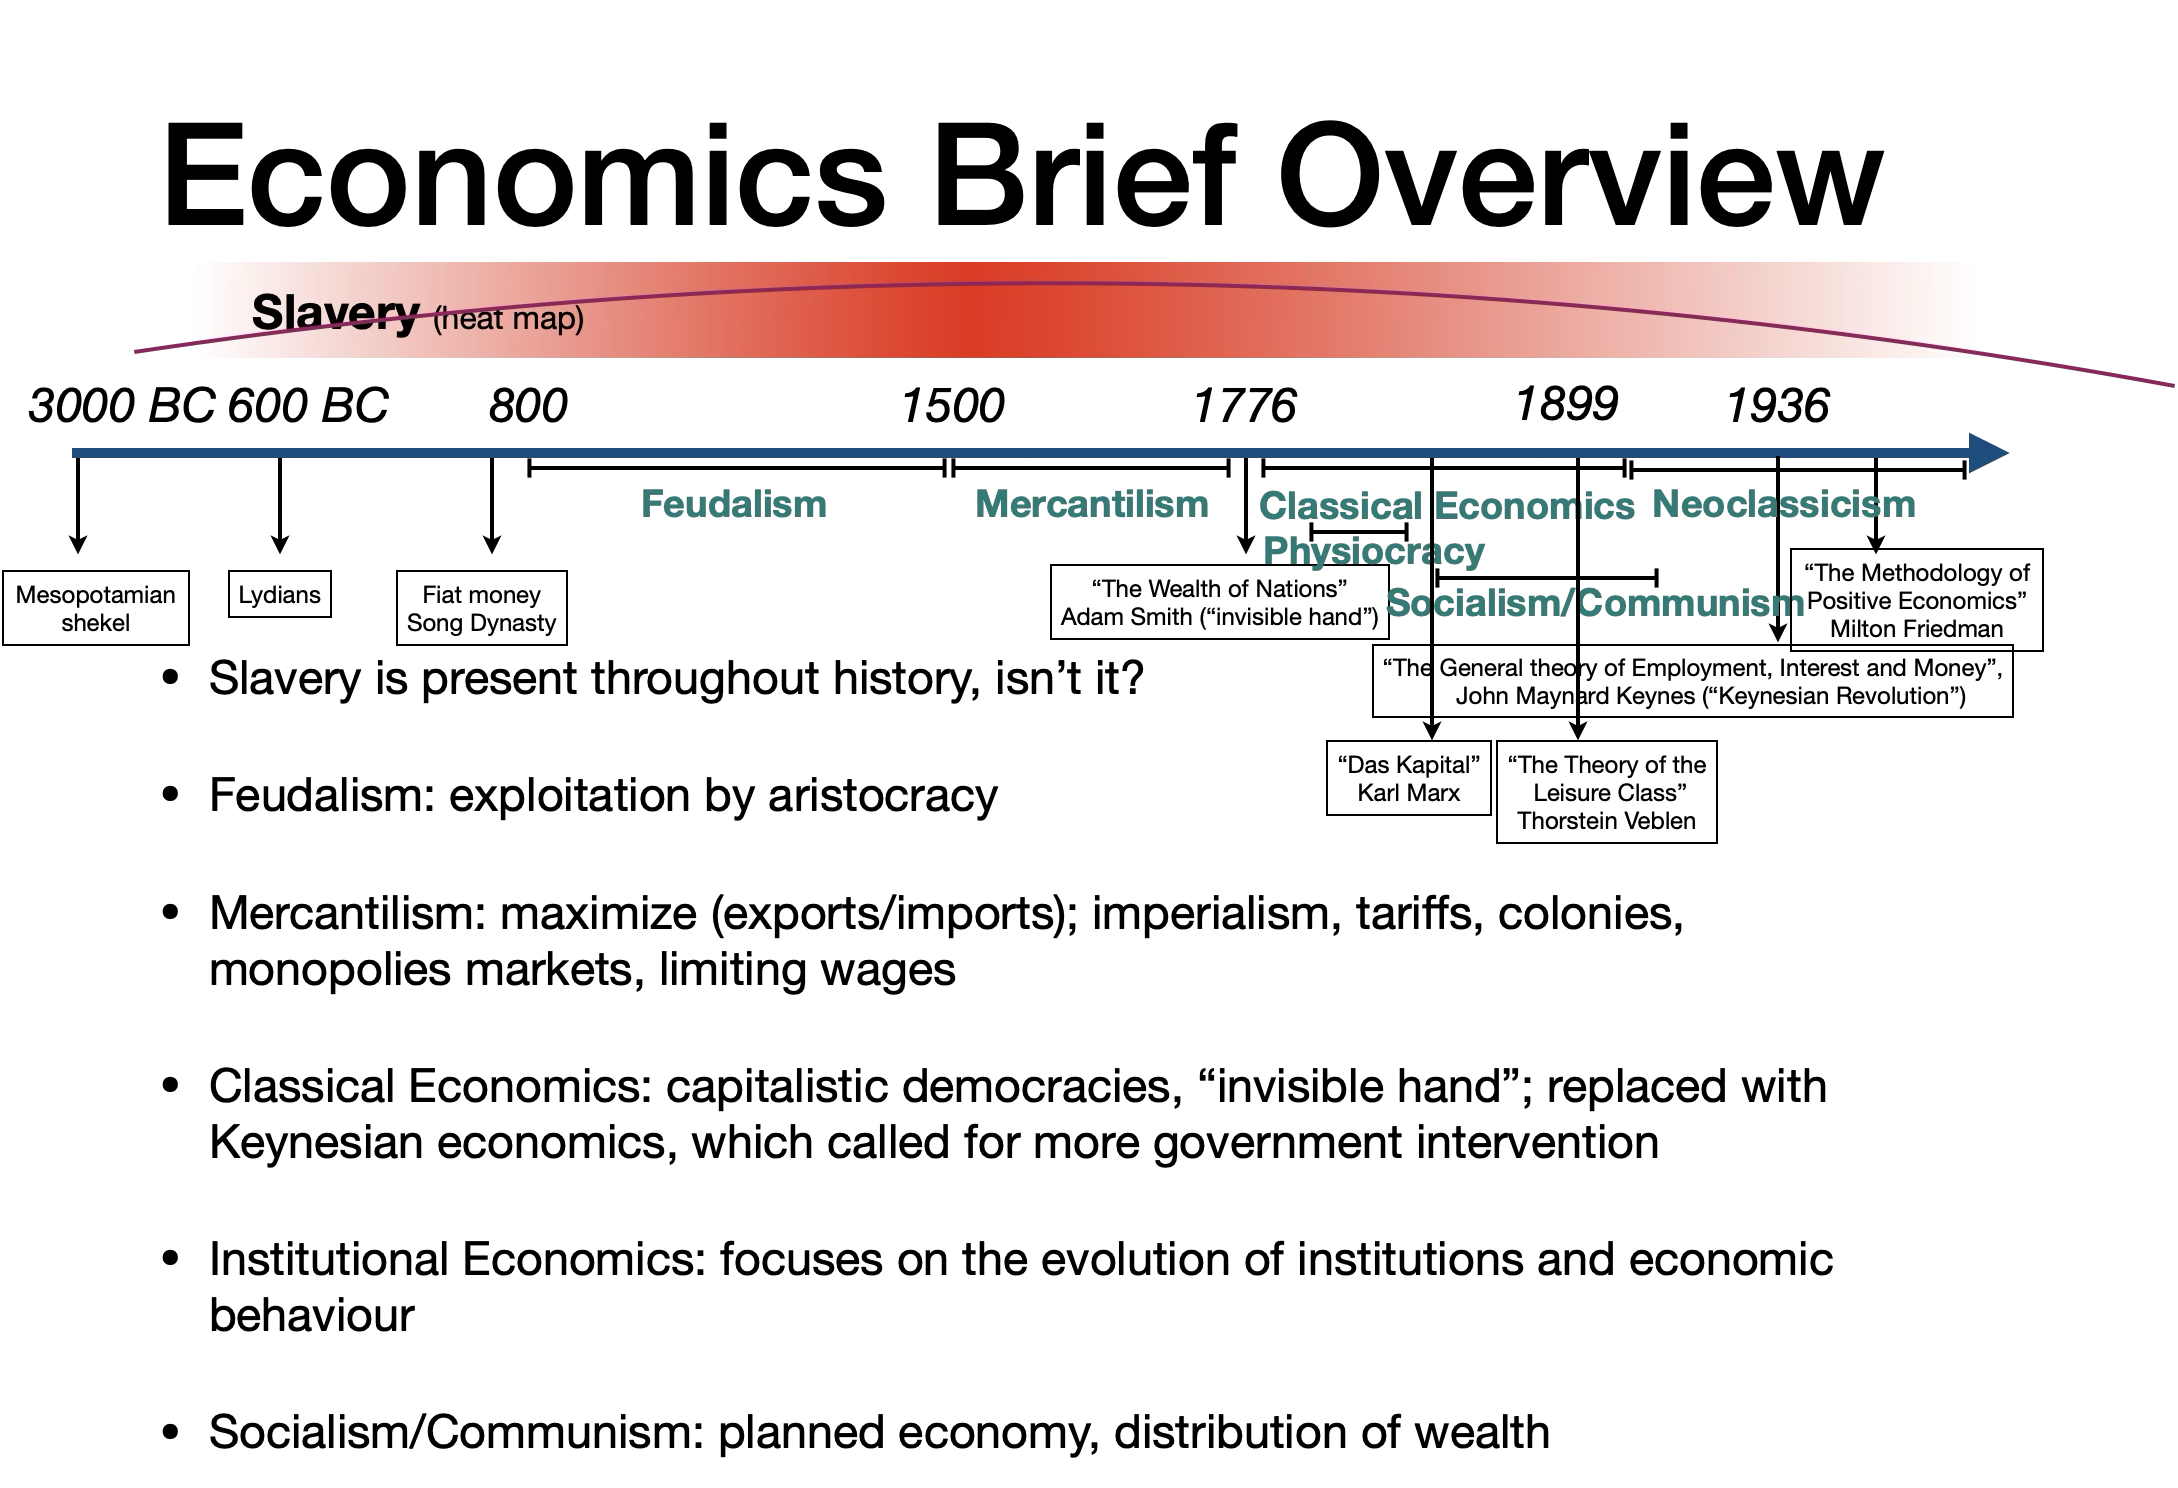
\includegraphics[width=0.9\textwidth]{fig/ses_overview.png}
    \caption{SES Overview: The multi-dimensional state space of human societies}
    \label{fig:ses_overview}
\end{figure}

\subsection{Motivation: Why Existing Metrics Fail}

Traditional economic indicators (GDP, unemployment rate, stock indices) provide a desperately incomplete picture of societal wellbeing. They are like measuring a human's health by only checking their bank account balance---technically a number, but missing everything that actually matters.

Similarly, happiness indices or social capital metrics capture important dimensions but lack the integrative framework needed to understand system dynamics. We need a formalism that:

\begin{enumerate}
    \item Includes economic, social, psychological, and spiritual dimensions
    \item Allows for mathematical modeling of dynamics and feedback loops  
    \item Provides measurable, empirically grounded parameters
    \item Reveals structural patterns invisible in single-domain analyses
\end{enumerate}

\SES{} is that formalism.

\subsection{Core Definition}

\begin{definition}[Socio-Economic-Spiritual State]\label{def:ses}
The \textbf{Socio-Economic-Spiritual State} (\SES) of a society at time $t$ is a point in a high-dimensional manifold $\mathcal{M}_{SES}$, parameterized by:

\begin{align}
\text{SES}(t) = \Big( &\mathbf{E}(t), \mathbf{S}(t), \mathbf{P}(t), \mathbf{C}(t), \mathbf{M}(t), \mathbf{I}(t), \mathbf{G}(t) \Big)
\end{align}

where:
\begin{itemize}[leftmargin=2cm]
    \item[$\mathbf{E}$:] \textbf{Economic parameters} (wealth distribution, production, resource flows)
    \item[$\mathbf{S}$:] \textbf{Social parameters} (trust, cooperation, community strength, violence rates)
    \item[$\mathbf{P}$:] \textbf{Psychological parameters} (wellbeing, meaning, mental health, stress)
    \item[$\mathbf{C}$:] \textbf{Consciousness parameters} (awareness levels, reflective capacity, wisdom)
    \item[$\mathbf{M}$:] \textbf{Material-Environmental} (resource health, ecological balance, sustainability)
    \item[$\mathbf{I}$:] \textbf{Institutional parameters} (governance quality, transparency, power distribution)
    \item[$\mathbf{G}$:] \textbf{Generational parameters} (intergenerational wellbeing transfer, future orientation)
\end{itemize}
\end{definition}

Each parameter vector itself contains multiple measurable components. For instance:

\begin{align}
\mathbf{E}(t) &= (W_{gini}(t), \text{GDP}(t), P_{capital}(t), U_{emp}(t), \ldots) \\
\mathbf{S}(t) &= (T_{trust}(t), C_{crime}(t), V_{civic}(t), R_{social}(t), \ldots) \\
\mathbf{P}(t) &= (H_{happiness}(t), M_{meaning}(t), D_{depression}(t), S_{suicide}(t), \ldots)
\end{align}

where subscripts denote specific metrics (e.g., $W_{gini}$ = Gini coefficient, $T_{trust}$ = generalized trust index, $M_{meaning}$ = meaning in life scores).

\begin{figure}[H]
    \centering
    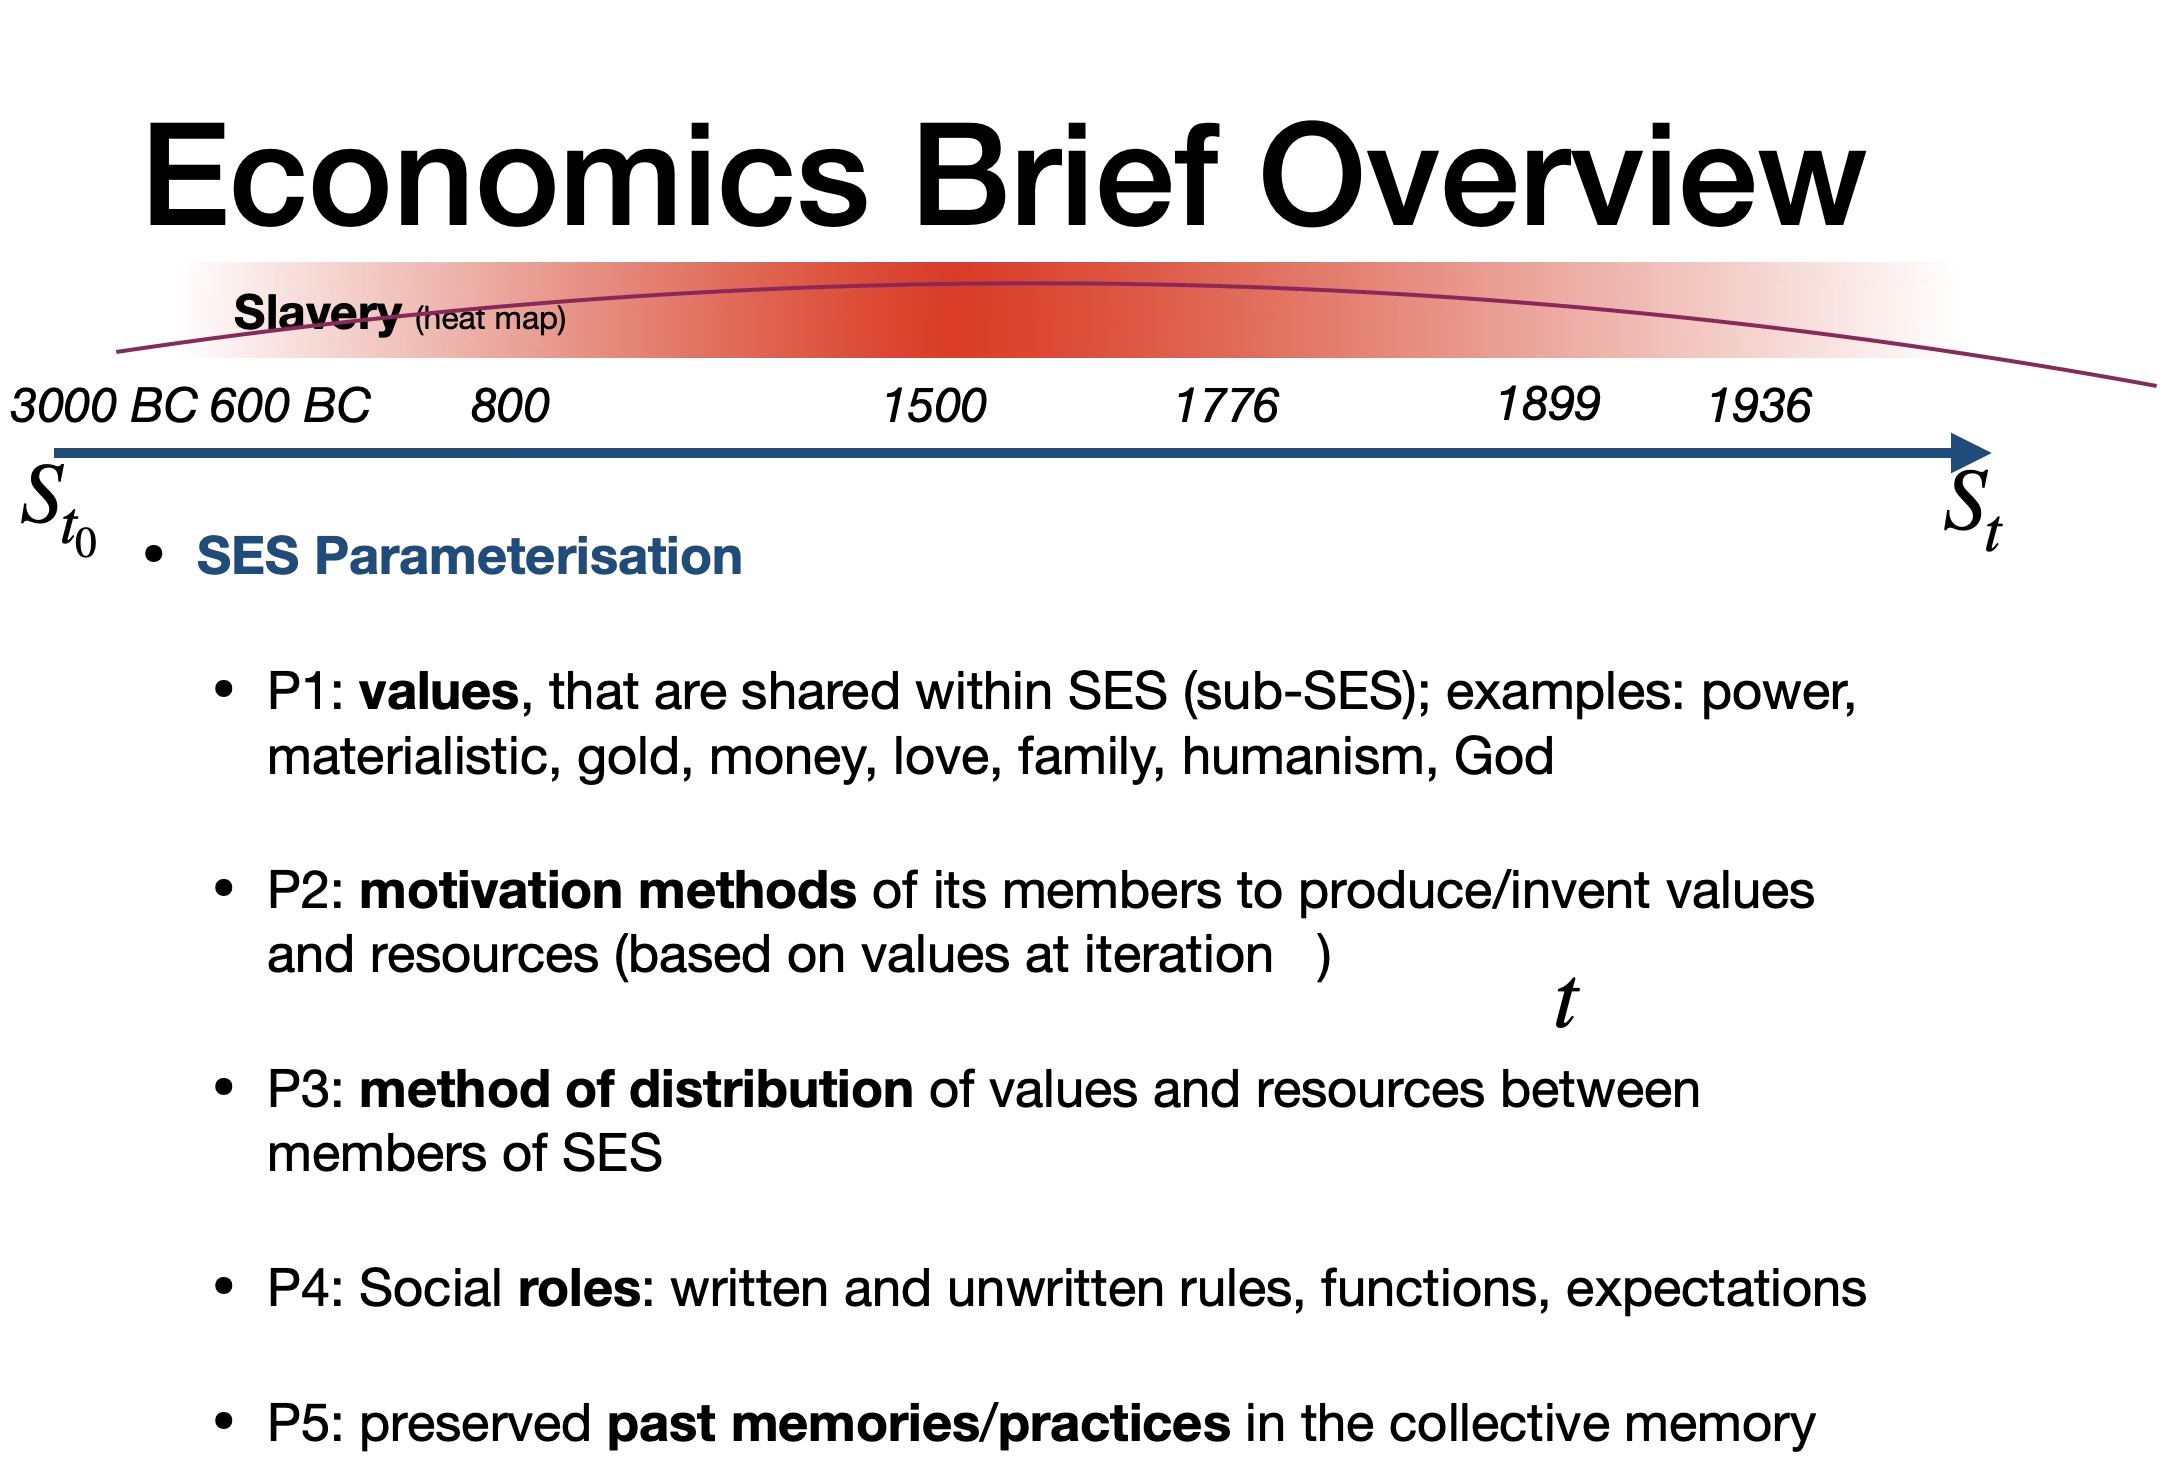
\includegraphics[width=0.95\textwidth]{fig/ses_parameterisation.png}
    \caption{SES Parameterization: Detailed breakdown of measurement dimensions}
    \label{fig:ses_parameters}
\end{figure}

\subsection{The Human as SES Mosaic}

Just as societies have \SES{} states, so do individuals. Each person is a complex mosaic of socio-economic-spiritual parameters that both reflects and contributes to the collective state.

\begin{figure}[H]
    \centering
    \includegraphics[width=0.75\textwidth]{fig/human_as_mosaic_ses_dna.png}
    \caption{The human as SES mosaic: individual parameters that aggregate into collective patterns}
    \label{fig:human_mosaic}
\end{figure}

This bi-directional relationship---individual $\leftrightarrow$ collective---is crucial. SYSTEM operates at both levels simultaneously:

\begin{itemize}
    \item \textbf{Top-down:} Institutional structures shape individual consciousness and behavior
    \item \textbf{Bottom-up:} Individual unconsciousness aggregates into systemic patterns
    \item \textbf{Resonance:} Feedback loops amplify small deviations into large shifts
\end{itemize}

\subsection{SES Dynamics and Evolution}

\SES{} is not static. It evolves according to complex dynamics:

\begin{equation}
\frac{d\text{SES}}{dt} = F(\text{SES}, \text{History}, \text{External}) + \text{Noise}
\end{equation}

where:
\begin{itemize}
    \item $F$ encodes the system's internal dynamics (feedback loops, reinforcing mechanisms)
    \item History represents path-dependence (hysteresis, institutional memory)
    \item External includes exogenous shocks (climate events, technological disruptions)
    \item Noise captures irreducible randomness and individual agency
\end{itemize}

\begin{figure}[H]
    \centering
    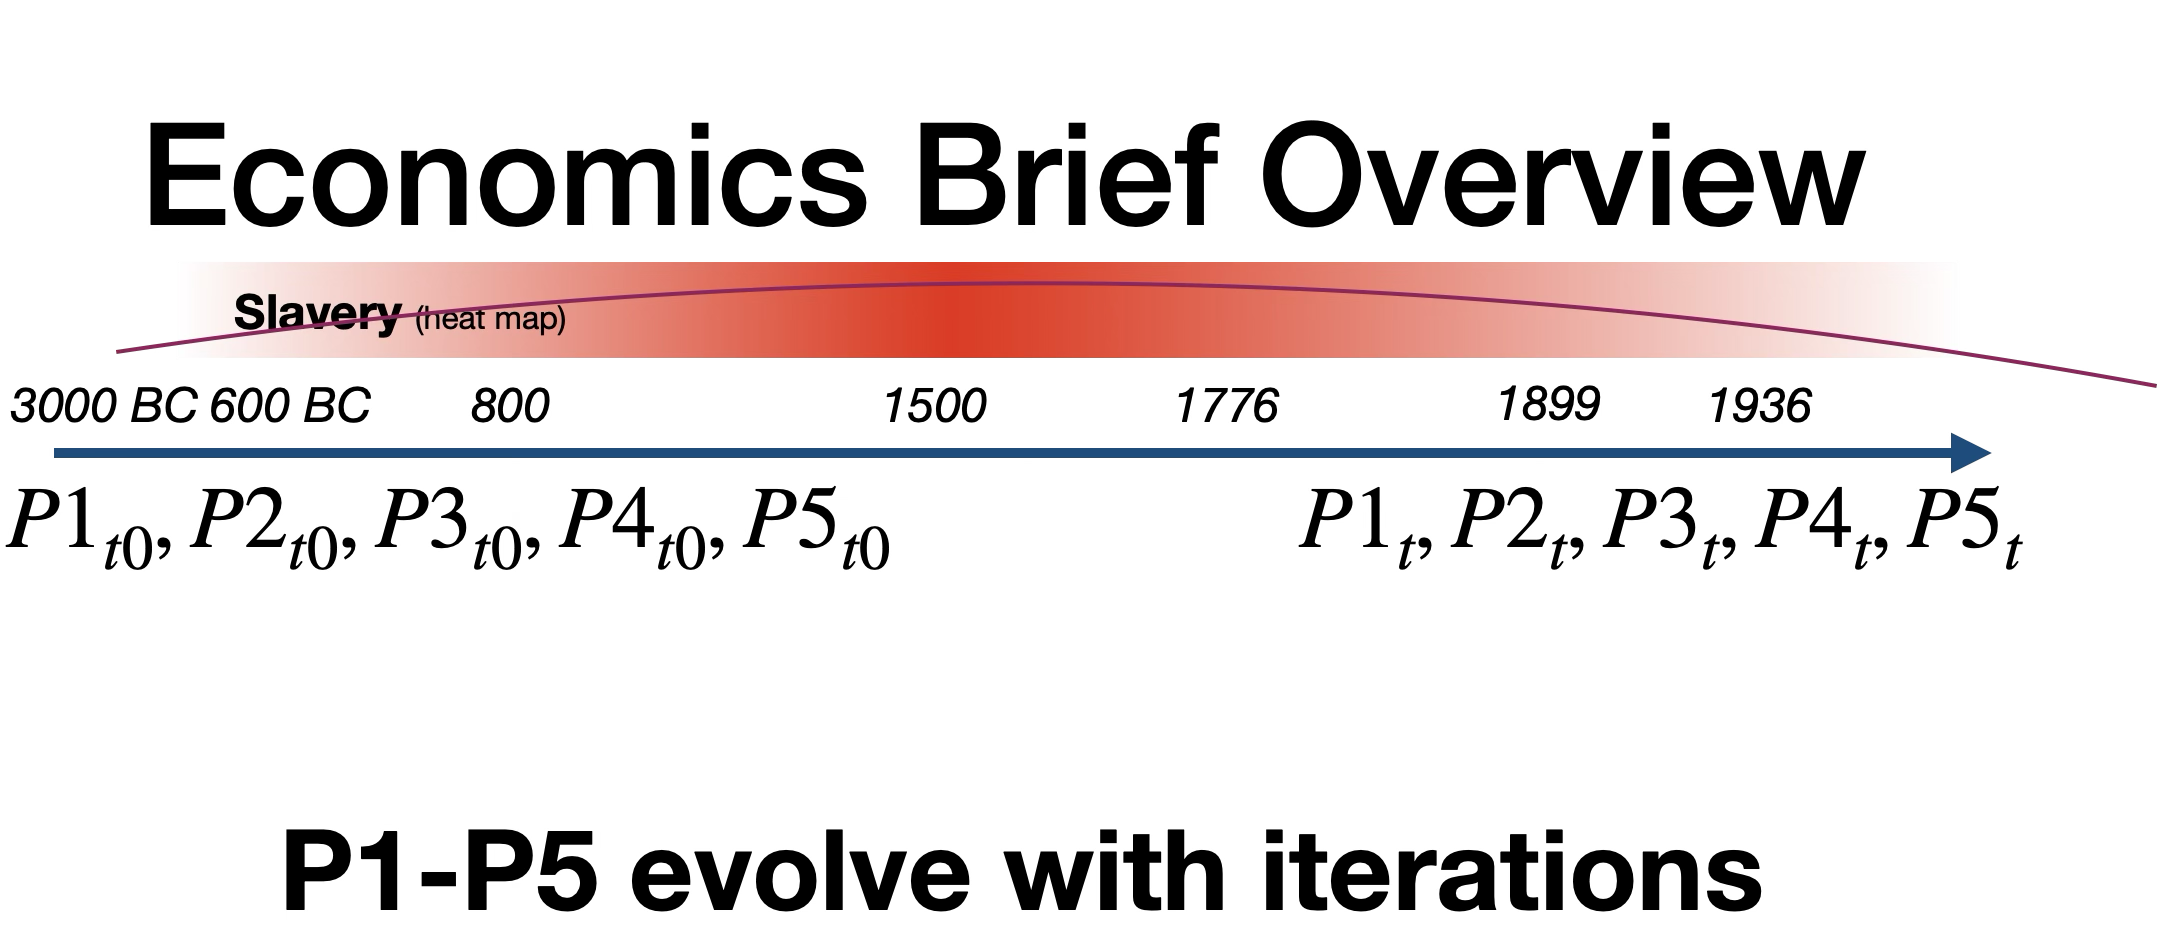
\includegraphics[width=0.9\textwidth]{fig/ses_params_evolution.png}
    \caption{SES parameter evolution over time: tracking societal transformation}
    \label{fig:ses_evolution}
\end{figure}

\subsection{Key Properties of SES Space}

The manifold $\mathcal{M}_{SES}$ has important geometric properties:

\begin{proposition}[Non-uniform Metric]\label{prop:ses_metric}
The space $\mathcal{M}_{SES}$ is equipped with a non-uniform Riemannian metric $g$, where distances between states reflect the ``cost'' (effort, time, suffering) required for transformation.
\end{proposition}

This means: some transitions are easier than others. Moving from high inequality to moderate inequality may be relatively straightforward. But escaping a trapped state (e.g., chronic dictatorship) requires overcoming potential barriers.

\begin{proposition}[Attractor States]\label{prop:attractors}
$\mathcal{M}_{SES}$ contains attractor regions corresponding to stable socio-economic configurations. Some attractors are \textit{healthy} (high wellbeing, sustainable), others are \textit{pathological} (high suffering, deteriorating).
\end{proposition}

SYSTEM is a pathological attractor. Once a society enters its basin of attraction, self-reinforcing dynamics pull it deeper---unless conscious intervention disrupts the pattern.

\begin{figure}[H]
    \centering
    \includegraphics[width=0.8\textwidth]{fig/ses_fractals.png}
    \caption{SES fractal structure: self-similar patterns across scales from individual to civilization}
    \label{fig:ses_fractals}
\end{figure}

\subsection{Connection to Consciousness Theory}

The consciousness parameters $\mathbf{C}(t)$ deserve special attention. We model consciousness as awareness operating on multiple levels:

\begin{align}
\mathbf{C}(t) = \Big( &C_{\text{individual}}(t), C_{\text{collective}}(t), C_{\text{institutional}}(t) \Big)
\end{align}

where each component can be further decomposed into:
\begin{itemize}
    \item \textit{Awareness depth:} How much of reality is perceived (vs. filtered by unconscious patterns)
    \item \textit{Reflective capacity:} Ability to examine one's own thinking and assumptions
    \item \textit{Integration:} Degree of internal coherence (vs. fragmentation/dissociation)
    \item \textit{Wisdom:} Ability to act in alignment with deep understanding
\end{itemize}

\begin{figure}[H]
    \centering
    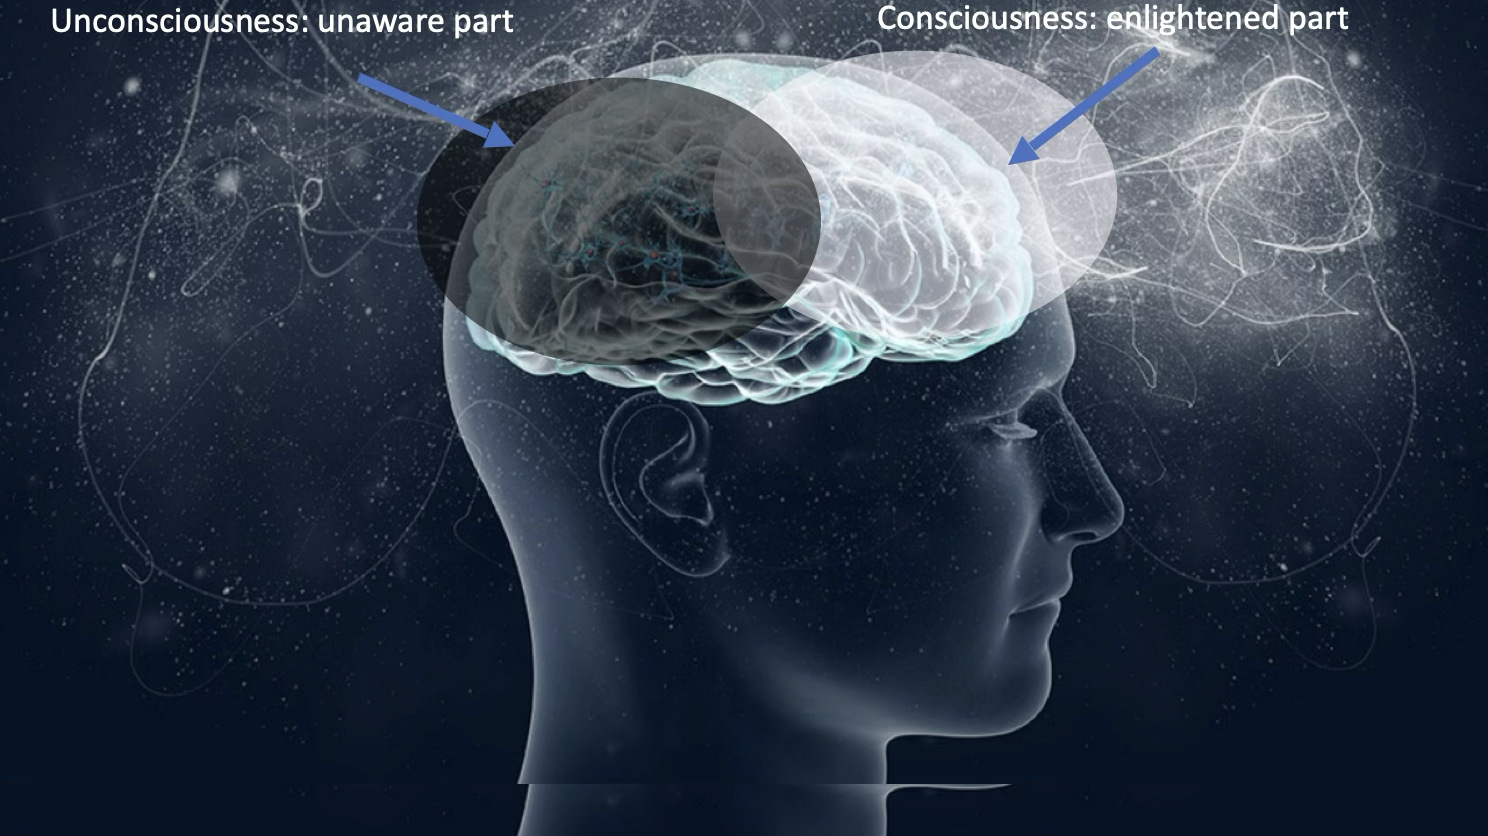
\includegraphics[width=0.85\textwidth]{fig/conciousness_subconciousness_model_eng.png}
    \caption{Consciousness-Subconsciousness model: the iceberg of awareness}
    \label{fig:consciousness_iceberg}
\end{figure}

The relationship between consciousness and other \SES{} parameters is \textit{not} symmetrical. While all parameters influence each other, consciousness has a special role: it is the only parameter that can \textit{intentionally modify the dynamics themselves}.

\begin{keyinsight}{Consciousness as Meta-Parameter}
Consciousness is the ``steering wheel'' of \SES{} evolution. All other parameters respond to forces; consciousness can \textit{choose} responses. This is why individual and collective consciousness development is not merely one intervention among many---it is the \textit{prerequisite} for all lasting transformation.
\end{keyinsight}

% ==================== PART 1 CONTINUED ====================

\section{SYSTEM: The Self-Reinforcing Pattern of Unconsciousness}

Now we can formally define SYSTEM---the pathological attractor that characterizes much of modern civilization.

\subsection{Formal Definition}

\begin{definition}[SYSTEM]\label{def:system}
\textbf{SYSTEM} is a self-reinforcing socio-economic-spiritual configuration characterized by:

\begin{enumerate}
    \item \textbf{Unconscious Operation:} Core dynamics driven by unexamined assumptions and automated patterns rather than conscious choice
    
    \item \textbf{Extractive Economics:} Value flows systematically from many to few, from future to present, from living systems to inert capital
    
    \item \textbf{Dehumanization Gradient:} Progressive treatment of humans as resources/inputs rather than conscious beings with intrinsic worth
    
    \item \textbf{Meaning Void:} Systematic replacement of intrinsic meaning with instrumental metrics (money, status, consumption)
    
    \item \textbf{Self-Reinforcement:} Mechanisms that amplify deviations toward greater unconsciousness, inequality, and suffering
    
    \item \textbf{Collective Blindness:} Structural barriers to seeing the system itself (like fish not seeing water)
\end{enumerate}
\end{definition}

Think of SYSTEM as a strange attractor in SES space---a region where trajectories converge and circle endlessly, unable to escape without external perturbation. But unlike the Lorenz attractor (which is aesthetically beautiful), this attractor generates suffering.

\subsection{Mathematical Formalization}

We can express SYSTEM mathematically as a region $\Omega_{SYSTEM} \subset \mathcal{M}_{SES}$ defined by:

\begin{equation}
\Omega_{SYSTEM} = \left\{ \text{SES} \in \mathcal{M}_{SES} \,:\, \delta(\text{SES}) > \delta_{critical} \right\}
\end{equation}

where $\delta(\text{SES})$ is the \textbf{\deltaDehum{} index}, measuring the degree of dehumanization present in the state, and $\delta_{critical}$ is a threshold beyond which self-reinforcing deterioration dominates.

\begin{definition}[$\delta$-Dehumanization Index]\label{def:delta}
The \deltaDehum{} index quantifies the extent to which a society treats humans as means rather than ends:

\begin{equation}
\delta(\text{SES}) = f\left( \frac{\text{Instrumental treatment}}{\text{Intrinsic worth recognition}}, \frac{\text{Extraction rate}}{\text{Regeneration rate}}, \frac{\text{Unconscious action}}{\text{Conscious choice}} \right)
\end{equation}

Operationally, $\delta$ can be estimated from observables:
\begin{itemize}
    \item Wealth concentration (Gini coefficient, top 1\% share)
    \item Worker autonomy and dignity indices
    \item Commodification extent (% of life domains governed by market logic)
    \item Attention capture and manipulation rates
    \item Environmental extraction vs. regeneration ratios
    \item Incarceration rates and punitive vs. restorative justice balance
\end{itemize}
\end{definition}

\begin{figure}[H]
    \centering
    
\includegraphics[width=0.85\textwidth]{fig/delta_dehumanisation_self_stimulating_circle.png}
    \caption{The $\delta$-dehumanization self-stimulating cycle: how small deviations compound into systemic patterns}
    \label{fig:delta_cycle}
\end{figure}

\subsection{The Dynamics of Delta}

The evolution of $\delta$ over time follows a feedback-dominated equation:

\begin{equation}
\frac{d\delta}{dt} = \alpha \delta^2 + \beta \delta + \gamma + \eta(t)
\end{equation}

where:
\begin{itemize}
    \item $\alpha > 0$: Self-reinforcement coefficient (dehumanization breeds more dehumanization)
    \item $\beta$: Linear drift term (systemic pressures)
    \item $\gamma$: Baseline tendency
    \item $\eta(t)$: Noise from individual agency and external shocks
\end{itemize}

This equation has critical implications:

\begin{theorem}[Runaway Dehumanization]\label{thm:runaway}
If $\delta > \delta^* = -\beta/(2\alpha)$, the system exhibits \textbf{runaway dehumanization}: $\delta \to \infty$ in finite time unless external intervention occurs.
\end{theorem}

\begin{proof}[Intuition]
The quadratic term dominates: as dehumanization increases, it accelerates its own growth. Like compound interest, but for suffering. The system crosses a point of no return where internal resistance mechanisms are overwhelmed by reinforcing loops.
\end{proof}

We are not claiming literal infinity---there are physical bounds (total collapse). But the theorem captures the qualitative reality: beyond a threshold, deterioration accelerates uncontrollably.

\subsection{Archetypal Examples: SYSTEM in Action}

To make SYSTEM concrete, consider archetypal manifestations:

\subsubsection{The Prison-Industrial Complex}

\begin{figure}[H]
    \centering
    \includegraphics[width=0.8\textwidth]{fig/prison_experiment_illustration_delta_dehumanisation_dynamics.png}
    \caption{The Prison Experiment: How systems shape individual behavior through role enforcement and dehumanization}
    \label{fig:prison_experiment}
\end{figure}

The Stanford Prison Experiment \citep{spe1973} demonstrated how quickly \textit{arbitrary role assignment} can induce extreme dehumanization. Guards became sadistic, prisoners became passive, within days---not because individuals were evil, but because the \textit{system structure} programmed behavior.

Scale this pattern to an entire society that:
\begin{itemize}
    \item Incarcerates 2.3 million people (US, highest rate globally)
    \item Profits from incarceration (private prisons, phone call monopolies, unpaid labor)
    \item Treats prisoners as inventory rather than humans undergoing rehabilitation
    \item Creates permanent underclass (felony records block employment, voting, housing)
\end{itemize}

This is SYSTEM: a self-reinforcing loop where:
\begin{equation}
\text{Poverty} \xrightarrow{\text{crime}} \text{Incarceration} \xrightarrow{\text{record}} \text{Unemployability} \xrightarrow{\text{desperation}} \text{More poverty}
\end{equation}

And at each step, humans are treated as problems to be managed rather than conscious beings to be supported.

\subsubsection{The Attention Economy}

\begin{figure}[H]
    \centering
    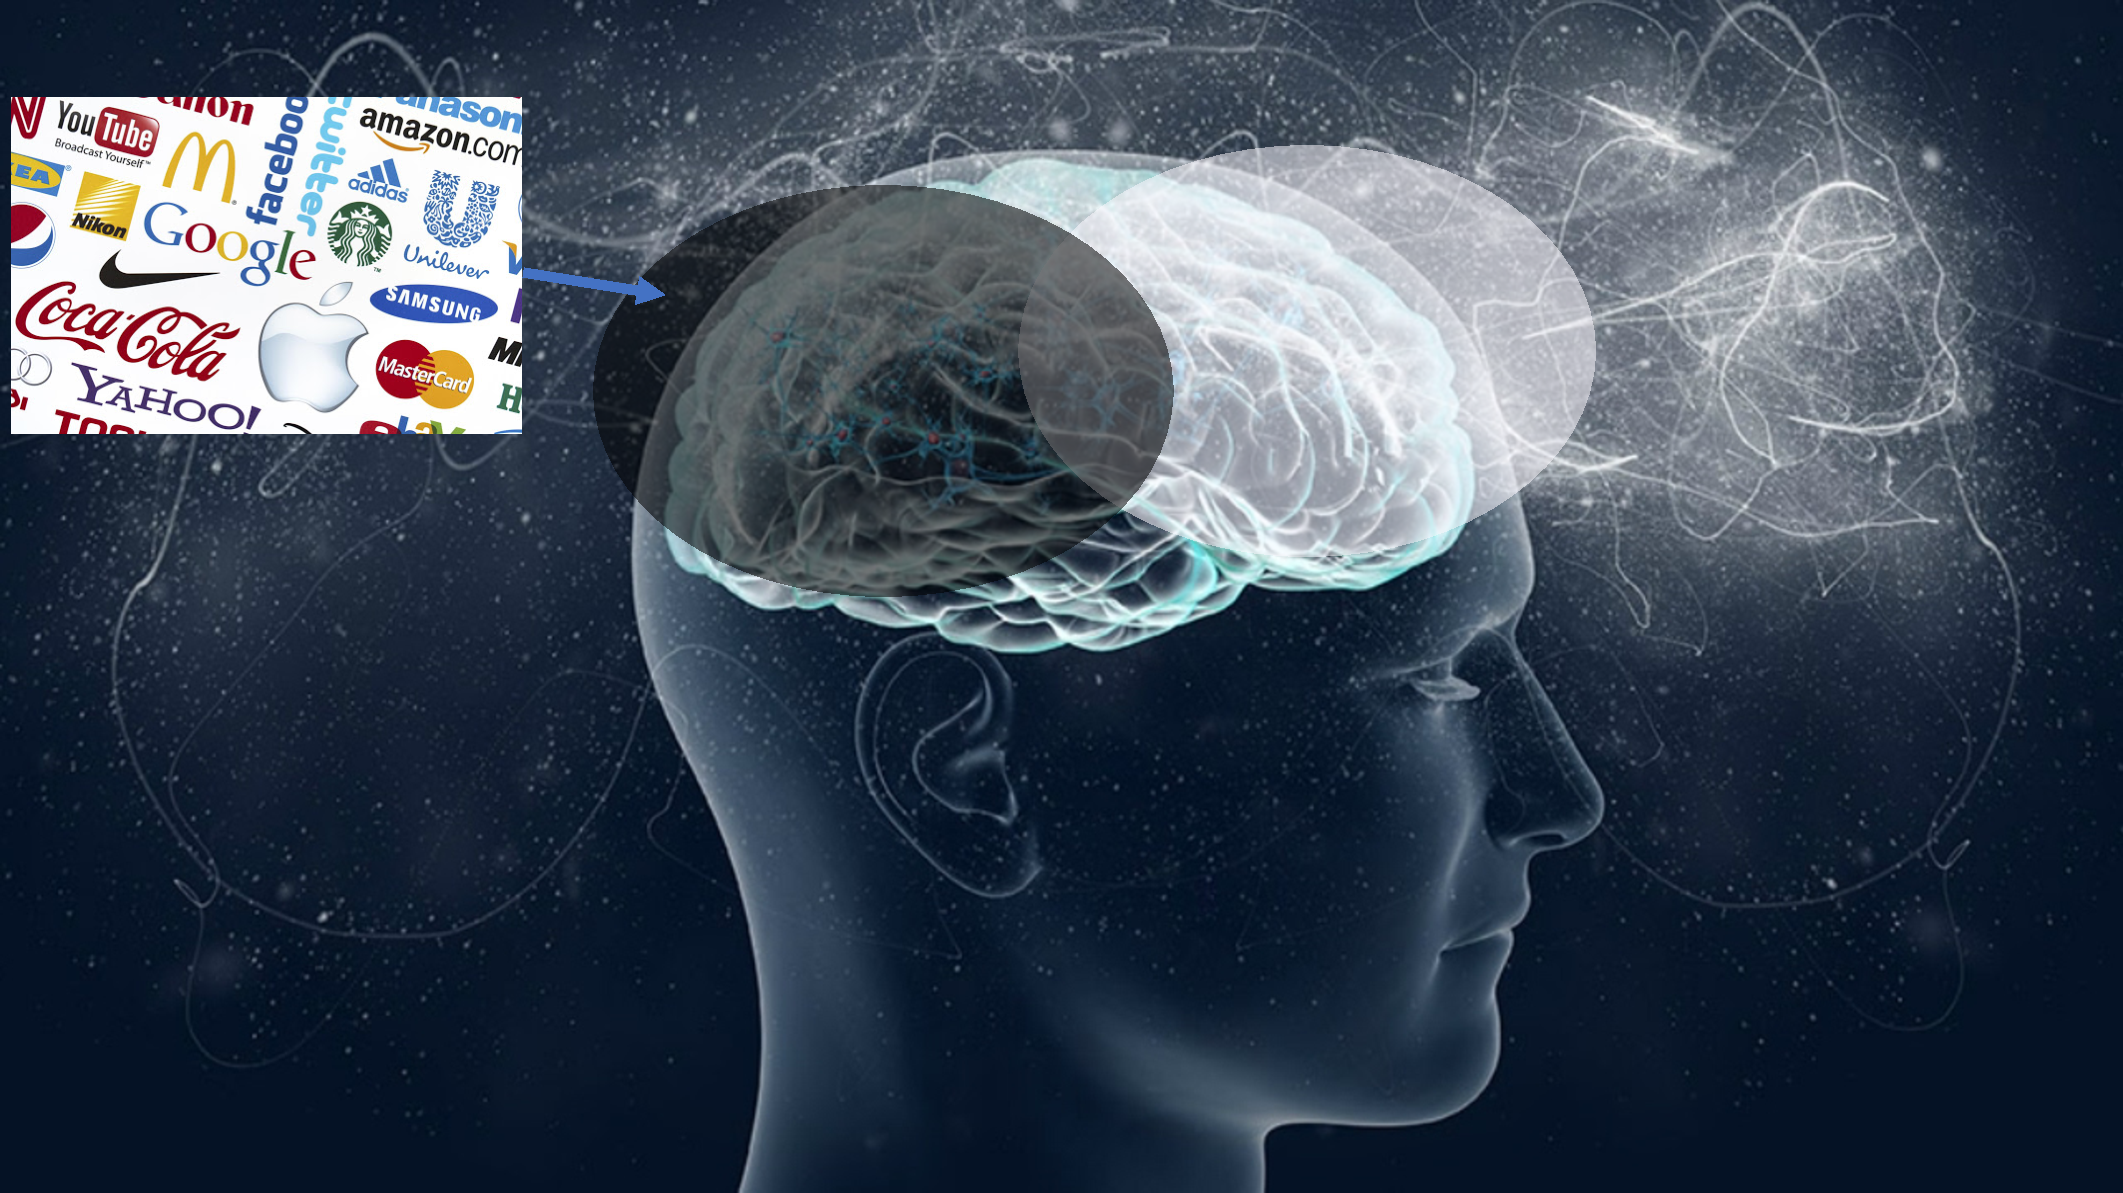
\includegraphics[width=0.85\textwidth]{fig/attention_economy_brands_as_real_estates_in_conciousness_space.png}
    \caption{Brands as real estate in consciousness space: the colonization of attention}
    \label{fig:attention_economy}
\end{figure}

Modern platforms (social media, streaming, infinite scroll) are engineered to maximize ``engagement''---a euphemism for attention capture. But attention is not merely a commodity; it is \textit{the raw material of consciousness}.

When your attention is continuously hijacked by algorithmic manipulation:
\begin{itemize}
    \item You cannot think deeply (constant interruption)
    \item You cannot feel genuinely (emotional buttons pushed for clicks)
    \item You cannot choose freely (your preferences are shaped by optimization systems)
    \item You cannot be present (always pulled into digital elsewhere)
\end{itemize}

This is dehumanization at the cognitive level: treating consciousness as a resource to be mined for advertising revenue. Your inner life becomes real estate to be colonized.

The feedback loop:
\begin{equation}
\text{Attention capture} \to \text{Reduced autonomy} \to \text{Dependency} \to \text{More exposure} \to \text{Deeper capture}
\end{equation}

\subsubsection{The Wealth Extraction Machine}

\begin{figure}[H]
    \centering
    \includegraphics[width=0.9\textwidth]{fig/inequality.png}
    \caption{Inequality: The fundamental pattern of extractive systems}
    \label{fig:inequality_overview}
\end{figure}

Consider the mechanics of contemporary wealth concentration:

\begin{enumerate}
    \item \textbf{Capital returns exceed wage growth:} $r > g$ \citep{piketty2014capital}. If you own capital, your wealth compounds. If you sell labor, you fall behind. The gap widens automatically.
    
    \item \textbf{Compound interest on wealth:} Even with modest 7\% annual returns, wealth doubles every 10 years. Over 40 years, \$1M becomes \$16M. Meanwhile, wages are flat.
    
    \item \textbf{Legislative capture:} The wealthy fund politicians who pass favorable tax laws. Lower capital gains taxes, offshore havens, carried interest loopholes. Democracy becomes plutocracy.
    
    \item \textbf{Intergenerational transfer:} Wealth dynasties persist across centuries. The rich don't just win once; they ensure their descendants never need to compete.
\end{enumerate}

\begin{figure}[H]
    \centering
    \begin{subfigure}[b]{0.48\textwidth}
        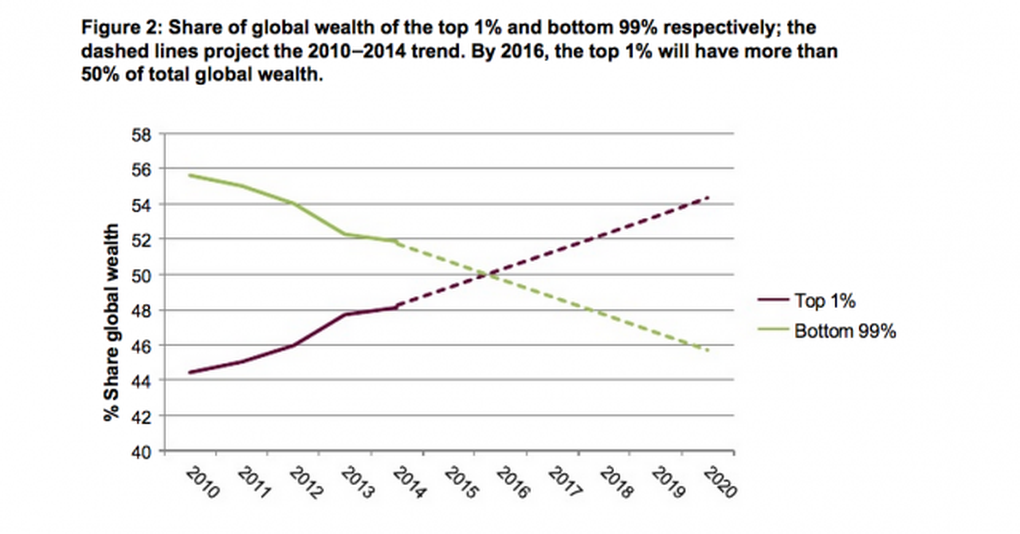
\includegraphics[width=\textwidth]{fig/inequality_graph_dynamics.png}
        \caption{Inequality dynamics over time}
    \end{subfigure}
    \hfill
    \begin{subfigure}[b]{0.48\textwidth}
        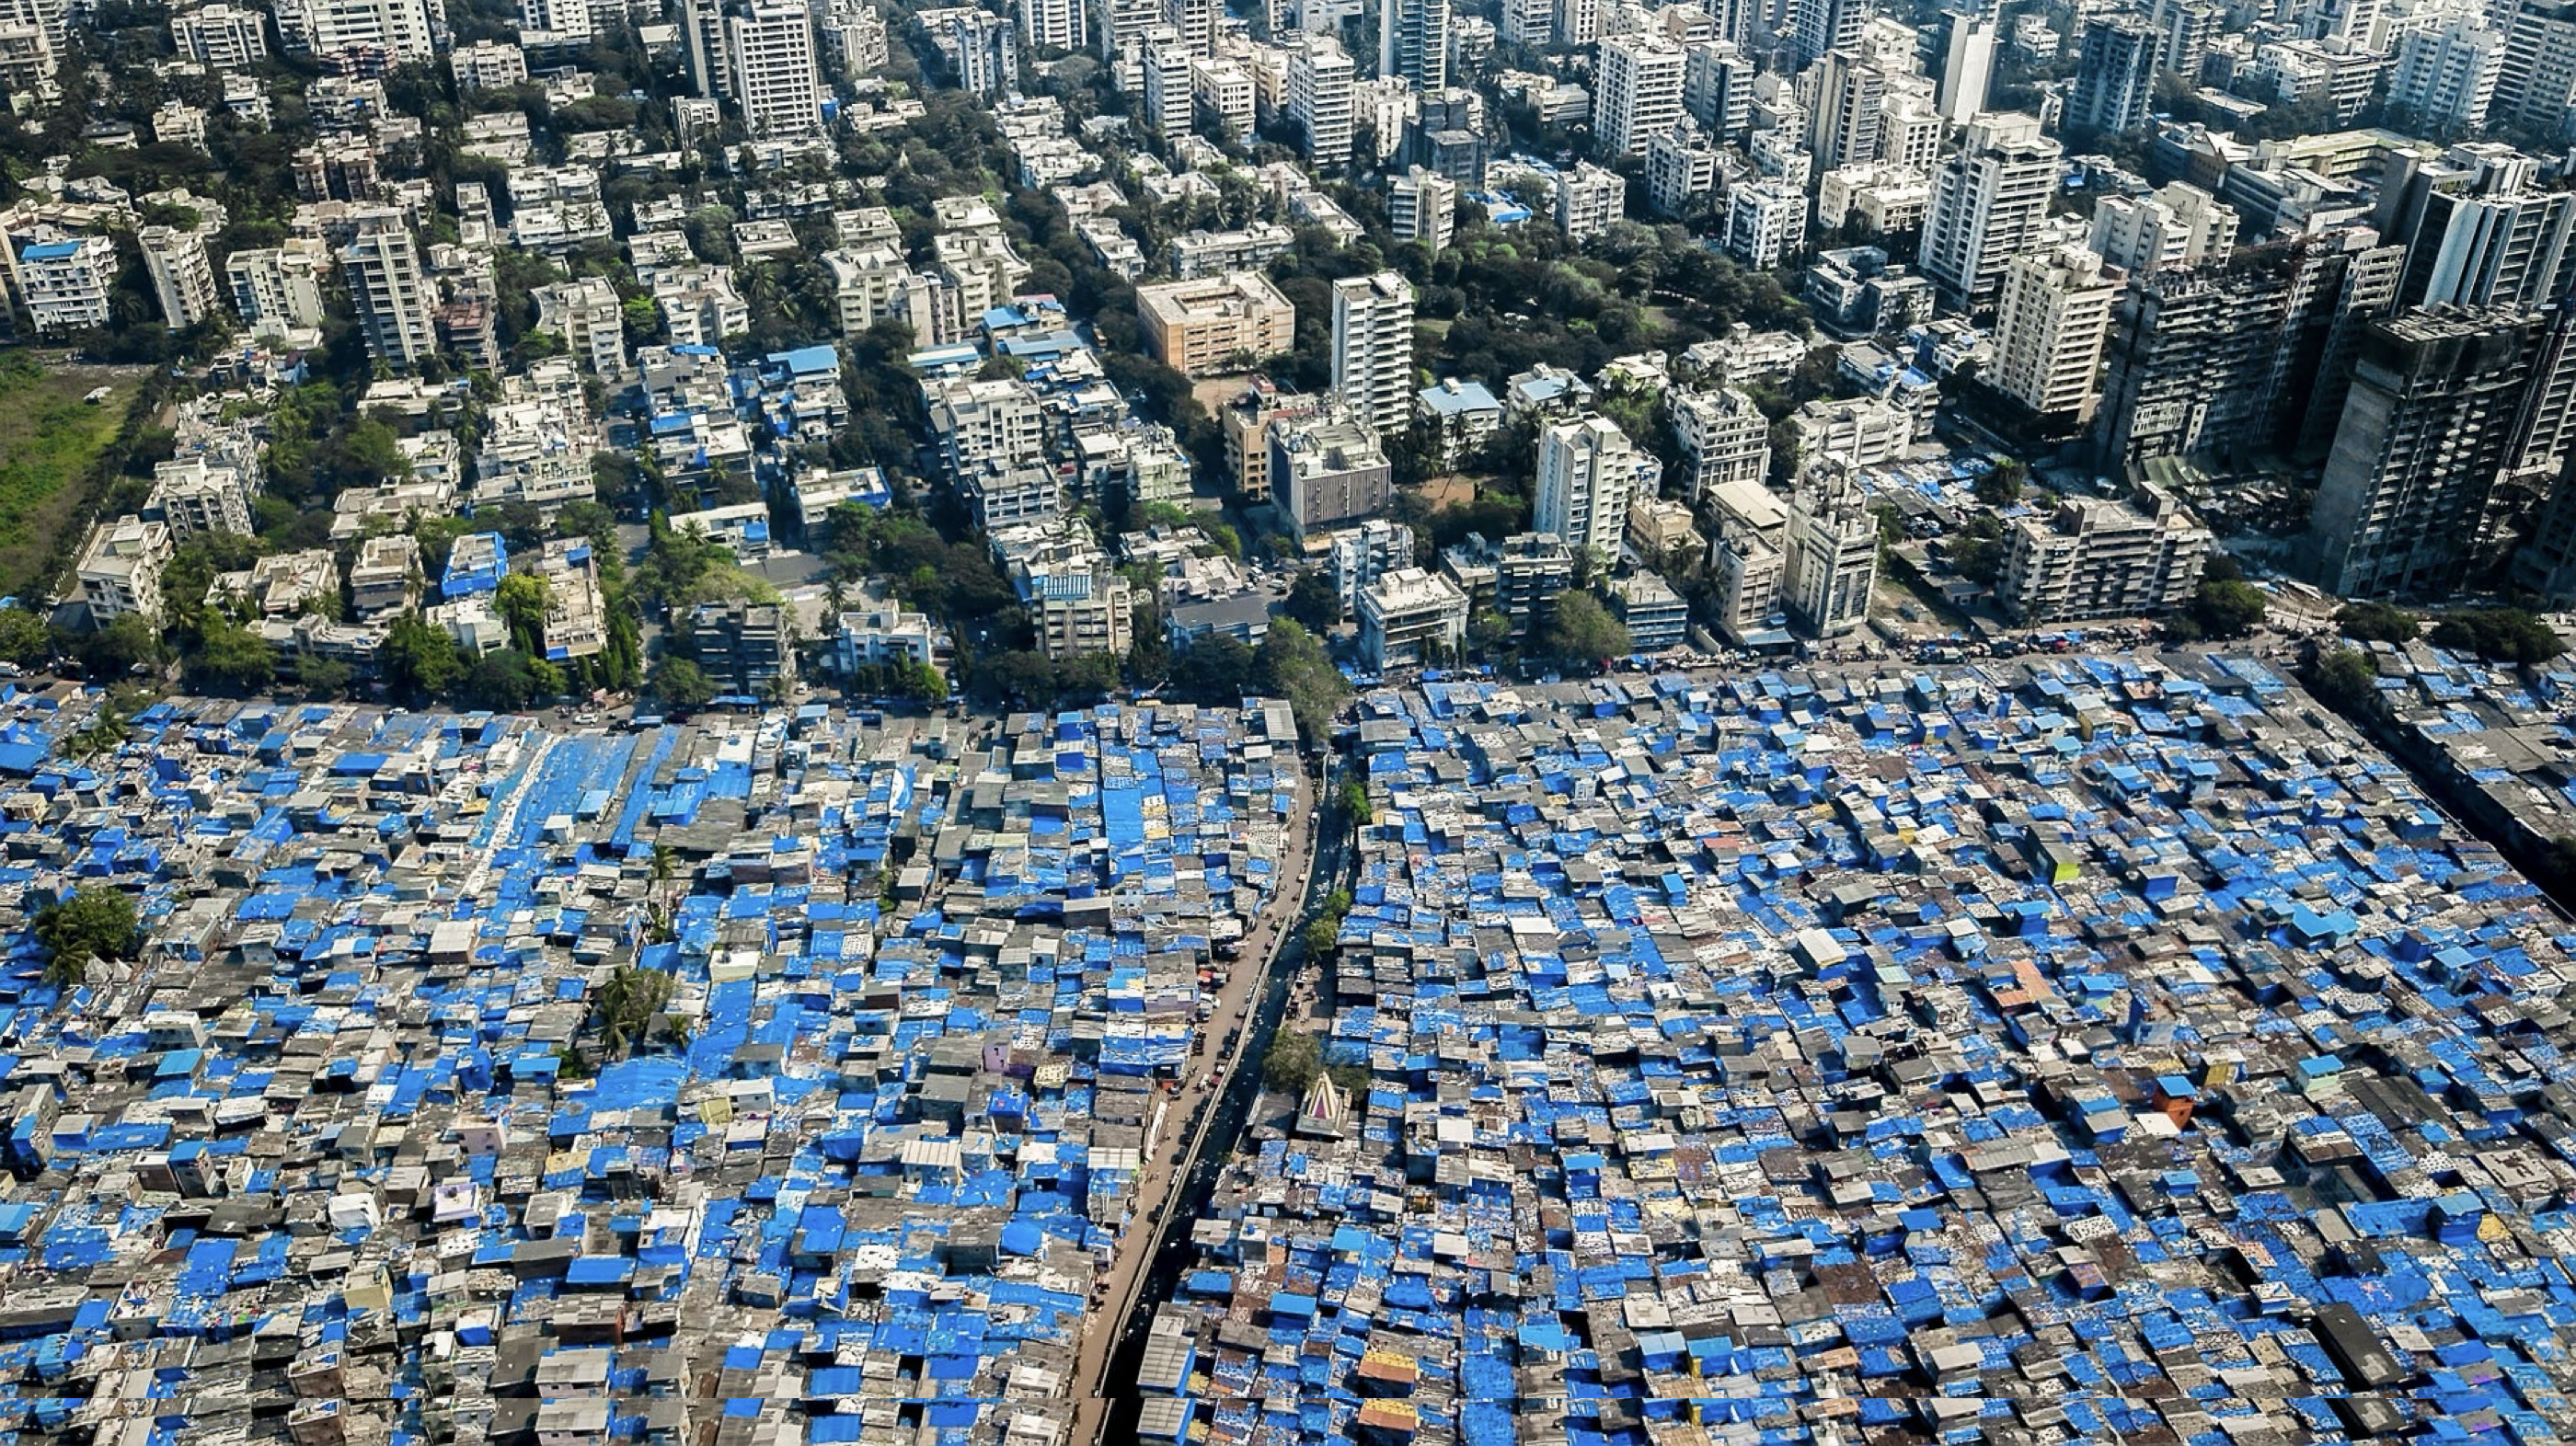
\includegraphics[width=\textwidth]{fig/inequality_illustration.png}
        \caption{Visual representation of wealth distribution}
    \end{subfigure}
    \caption{Tracking inequality: quantitative and qualitative perspectives}
    \label{fig:inequality_details}
\end{figure}

Result: In 2024, the top 1\% own more than the bottom 50\% globally. Not because they work 1000x harder, but because SYSTEM is \textit{designed} to funnel wealth upward.

\subsubsection{The Snake Eating Itself}

\begin{figure}[H]
    \centering
    \includegraphics[width=0.7\textwidth]{fig/zmeya_poedaet_sebya_illustration_of_dynamics.png}
    \caption{The ouroboros of SYSTEM: self-consumption leading to collapse}
    \label{fig:ouroboros}
\end{figure}

SYSTEM ultimately destroys its own foundations:
\begin{itemize}
    \item Extracts resources faster than regeneration $\Rightarrow$ ecological collapse
    \item Concentrates wealth $\Rightarrow$ demand collapses $\Rightarrow$ economic crisis
    \item Erodes meaning $\Rightarrow$ mental health epidemic $\Rightarrow$ productivity collapse
    \item Undermines trust $\Rightarrow$ institutions fail $\Rightarrow$ coordination impossible
\end{itemize}

Like a parasite that kills its host, SYSTEM is not sustainable. But unlike biological parasites (which evolve toward less lethality), SYSTEM has no built-in corrective mechanism. It will consume until collapse unless \textit{conscious intervention} interrupts the pattern.

\subsection{The Parent Metaphor: Top 1\% as Collective Parent}

Here's a useful analogy: Imagine humanity as a large family, and the top 1\% (by wealth, power, influence) as the \textit{parents}. What kind of parents are they?

\begin{figure}[H]
    \centering
    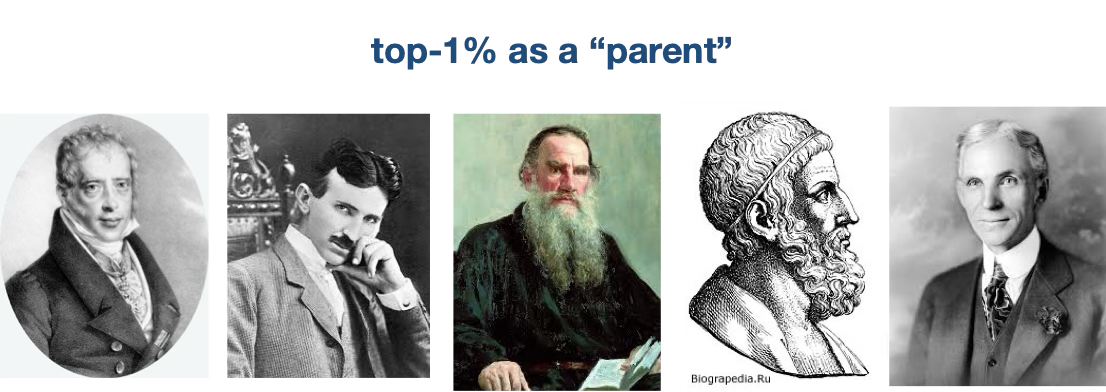
\includegraphics[width=0.75\textwidth]{fig/top1percent_as_Parent_for_Humanity.png}
    \caption{The top 1\% as Parent for Humanity: modeling elite influence on collective development}
    \label{fig:parent_metaphor}
\end{figure}

\begin{itemize}
    \item \textbf{Neglectful?} They hoard resources while children go hungry (literal starvation in poor regions, metaphorical starvation of meaning/opportunity in rich ones)
    
    \item \textbf{Abusive?} They exploit labor, manipulate attention, extract value without reciprocity
    
    \item \textbf{Gaslighting?} They fund think tanks to claim inequality is natural/necessary, that climate change is debatable, that people are poor due to personal failure
    
    \item \textbf{Absent?} They live in isolated bubbles (gated communities, private islands), disconnected from the consequences of their decisions
\end{itemize}

\begin{figure}[H]
    \centering
    \includegraphics[width=0.7\textwidth]{fig/parents_top1percent.png}
    \caption{Parental archetypes and their impact on collective development}
    \label{fig:parent_types}
\end{figure}

This is not to claim that wealthy individuals are personally evil. Many are unconscious---they inherited roles and systems without questioning them. The point is \textit{structural}: when power is concentrated, those who wield it become de facto parents to everyone else. And currently, they are failing that role catastrophically.

A healthy parent:
\begin{itemize}
    \item Ensures all children have basic needs met
    \item Creates conditions for each child to develop their unique potential
    \item Models wisdom, integrity, and care
    \item Prepares children to eventually become self-sufficient adults
\end{itemize}

SYSTEM does the opposite: creates dependency, suppresses potential, models extraction, and perpetuates childhood (in the sense of powerlessness).

\subsection{Cognitive and Institutional Mechanisms}

SYSTEM operates through specific mechanisms at multiple levels:

\subsubsection{Individual Level: Consciousness Capture}

\begin{itemize}
    \item \textbf{Cognitive load exhaustion:} Keep people busy/stressed so they have no bandwidth for reflection
    \item \textbf{Preference fabrication:} Shape desires through marketing/propaganda so people want what serves SYSTEM
    \item \textbf{Identity attachment:} Bind self-worth to consumption/status so people defend their own exploitation
    \item \textbf{Learned helplessness:} Convince people change is impossible so they don't try
\end{itemize}

\subsubsection{Social Level: Divide and Distract}

\begin{itemize}
    \item \textbf{Fragmentation:} Pit groups against each other (race, politics, class) so they don't unite against structural injustice
    \item \textbf{Spectacle:} Provide endless entertainment so people don't notice the extraction
    \item \textbf{Manufactured consent:} Control media narratives to normalize the status quo
    \item \textbf{Tribalism exploitation:} Hijack in-group/out-group instincts for political manipulation
\end{itemize}

\subsubsection{Institutional Level: Structural Lock-In}

\begin{itemize}
    \item \textbf{Regulatory capture:} Industries regulate themselves through revolving doors with government
    \item \textbf{Legal frameworks favoring capital:} Property rights absolute, labor rights conditional
    \item \textbf{Complexity as moat:} Tax codes, financial instruments so complex that only specialists understand (and benefit)
    \item \textbf{Path dependence:} Infrastructure and institutions designed for extraction resist redesign
\end{itemize}

\subsection{Why SYSTEM Persists: The Stability Paradox}

A natural question: If SYSTEM is so destructive, why doesn't it collapse? Several factors:

\begin{enumerate}
    \item \textbf{Slow onset:} Like the frog in gradually heating water, changes happen too slowly to trigger alarm until it's late
    
    \item \textbf{Partial anesthesia:} SYSTEM provides just enough comfort/distraction to most people to prevent revolution (bread and circuses)
    
    \item \textbf{Collective action problems:} Individuals can't change system alone, coordination is hard
    
    \item \textbf{Cognitive dissonance resolution:} Easier to rationalize than confront (``this is just how the world works'')
    
    \item \textbf{Elite resistance:} Those benefiting have enormous power to resist change
    
    \item \textbf{Lack of viable alternatives:} Without clear alternative models, people accept what exists
\end{enumerate}

But crucially: \textbf{stability is not the same as sustainability}. SYSTEM is stable in the short term but catastrophic in the long term. Like standing on a slowly melting ice sheet---feels solid until suddenly it's not.

\section{The Geometry of the Fall: Consciousness Space and Trajectories}

Having defined SYSTEM formally, we now explore its geometric interpretation: humanity's trajectory through consciousness space, and what it means to ``fall.''

\subsection{The Consciousness Manifold}

Building on our earlier \SES{} framework, we now focus specifically on the consciousness dimension, which we model as a manifold $\mathcal{M}_C$.

\begin{definition}[Consciousness Manifold]\label{def:consciousness_manifold}
The \textbf{consciousness manifold} $\mathcal{M}_C$ is a pseudo-Riemannian manifold representing possible states of individual and collective consciousness. Points in $\mathcal{M}_C$ correspond to specific configurations of awareness, integration, and capacity for conscious action.
\end{definition}

\begin{figure}[H]
    \centering
    \includegraphics[width=0.85\textwidth]{fig/ses_theory_waves_frequencies.png}
    \caption{SES Theory: Waves and frequencies---modeling consciousness as vibrational patterns}
    \label{fig:consciousness_waves}
\end{figure}

Key properties of $\mathcal{M}_C$:

\begin{enumerate}
    \item \textbf{Non-Euclidean:} The space has curvature. Some directions are ``easier'' to move in than others (path dependence).
    
    \item \textbf{Hierarchical structure:} Higher levels of consciousness have access to more dimensions (think: 3D being can see 2D flatlanders, but not vice versa).
    
    \item \textbf{Attractive and repulsive regions:} Some states are attractor basins (hard to leave), others are unstable peaks (hard to stay on).
    
    \item \textbf{Non-linear metric:} Small movements in certain directions can cause large changes in experience/capability.
\end{enumerate}

\subsection{Geodesics and the Christ-Vector}

In Riemannian geometry, a \textit{geodesic} is the shortest path between two points (generalizing the notion of ``straight line'' to curved spaces). In $\mathcal{M}_C$, geodesics have special significance.

\begin{definition}[Consciousness Geodesic]\label{def:geodesic}
A \textbf{consciousness geodesic} is a path through $\mathcal{M}_C$ that maximizes growth in awareness while minimizing suffering (both for self and others). These are the ``most efficient'' paths of development.
\end{definition}

In S.V.E. IV \citep{sve4}, we introduced the \textbf{Christ-Vector} as the tangent vector field pointing along geodesics---the ``direction of Love'' at any point in consciousness space.

\begin{equation}
\vec{C}(\mathcal{C}) = \text{direction of maximum compassionate awareness growth}
\end{equation}

Think of it like a compass that always points toward your highest development---not in the sense of achievement or power, but in depth of understanding and capacity to reduce suffering.

\begin{remark}[Universal Ethics from Geometry]
This geometric formulation provides a \textit{universal ethics} without requiring specific religious or cultural assumptions. The ``good'' is that which moves along geodesics; the ``evil'' is that which deviates from them. This is not relativism (``everything is equal'') but rather \textit{geometric objectivity}: some paths genuinely minimize suffering and maximize flourishing, just as some paths between cities are genuinely shorter.
\end{remark}

\subsection{The Fall: Deviation from Geodesic Path}

Now we can define humanity's ``Fall'' precisely:

\begin{definition}[The Fall]\label{def:fall}
The \textbf{Fall} is humanity's historical deviation from geodesic paths in consciousness space. Starting from some initial state $\mathcal{C}_0$ (representing earlier, more integrated forms of human existence), humanity followed a trajectory $\gamma(t)$ that increasingly diverged from the geodesic $\gamma^*$ it could have followed.
\end{definition}

The ``distance'' from geodesic measures cumulative deviation:

\begin{equation}
\text{Fall-depth}(t) = \int_0^t d_{\mathcal{M}_C}(\gamma(s), \gamma^*(s)) \, ds
\end{equation}

where $d_{\mathcal{M}_C}$ is the distance metric on consciousness space.

\begin{figure}[H]
    \centering
    \begin{tikzpicture}[scale=1.2]
        % Draw axes
        \draw[->] (0,0) -- (8,0) node[right] {Time};
        \draw[->] (0,0) -- (0,6) node[above] {Consciousness Level};
        
        % Draw geodesic path (optimal)
        \draw[thick, blue, dashed] (0.5,1) .. controls (2,2.5) and (4,4) .. (7.5,5) 
            node[right] {Geodesic $\gamma^*$};
        
        % Draw actual path (with fall)
        \draw[thick, red] (0.5,1) .. controls (1.5,2) and (3,2.2) .. (4.5,1.8)
            .. controls (5.5,1.6) and (6.5,1.4) .. (7.5,1) 
            node[right] {Actual $\gamma$};
        
        % Mark key points
        \filldraw[black] (0.5,1) circle (2pt) node[below] {$\mathcal{C}_0$};
        \filldraw[blue] (7.5,5) circle (2pt);
        \filldraw[red] (7.5,1) circle (2pt) node[below right] {Current state};
        
        % Show deviation
        \draw[<->, thick, purple] (7.2,1.2) -- (7.2,4.8) node[midway, right] {Fall-depth};
        
        % Mark historical events
        \draw[gray, dotted] (2,0) -- (2,2.3) node[above] {\small Agricultural Rev.};
        \draw[gray, dotted] (4.5,0) -- (4.5,1.8) node[above] {\small Industrial Rev.};
        \draw[gray, dotted] (6.5,0) -- (6.5,1.4) node[above] {\small Digital Age};
    \end{tikzpicture}
    \caption{The Fall visualized: humanity's deviation from geodesic development path}
    \label{fig:fall_diagram}
\end{figure}

\subsection{Historical Inflection Points}

Several key transitions mark humanity's fall:

\subsubsection{Agricultural Revolution (10,000 BCE)}

The shift from hunter-gatherer to agricultural societies brought:
\begin{itemize}
    \item[$+$] Population growth, settled communities, technology accumulation
    \item[$-$] Hierarchy emergence, property, warfare intensification, slavery
    \item[$-$] Loss of leisure (foragers worked 15-20 hrs/week, farmers 60+)
    \item[$-$] Dietary decline (skeletal evidence shows worse nutrition)
\end{itemize}

Paradox: Agricultural revolution was materially ``progressive'' but consciousness-wise \textit{regressive} in many dimensions. More stuff, less freedom.

\subsubsection{Development of Money and Debt (3000 BCE)}

Money began as accounting tool but evolved into:
\begin{itemize}
    \item Abstraction layer separating value from tangible reality
    \item Enabler of compound interest and wealth accumulation
    \item Mechanism for transforming humans into debtors (slaves to obligation)
    \item Universal equivalence destroying qualitative distinction
\end{itemize}

\begin{figure}[H]
    \centering
    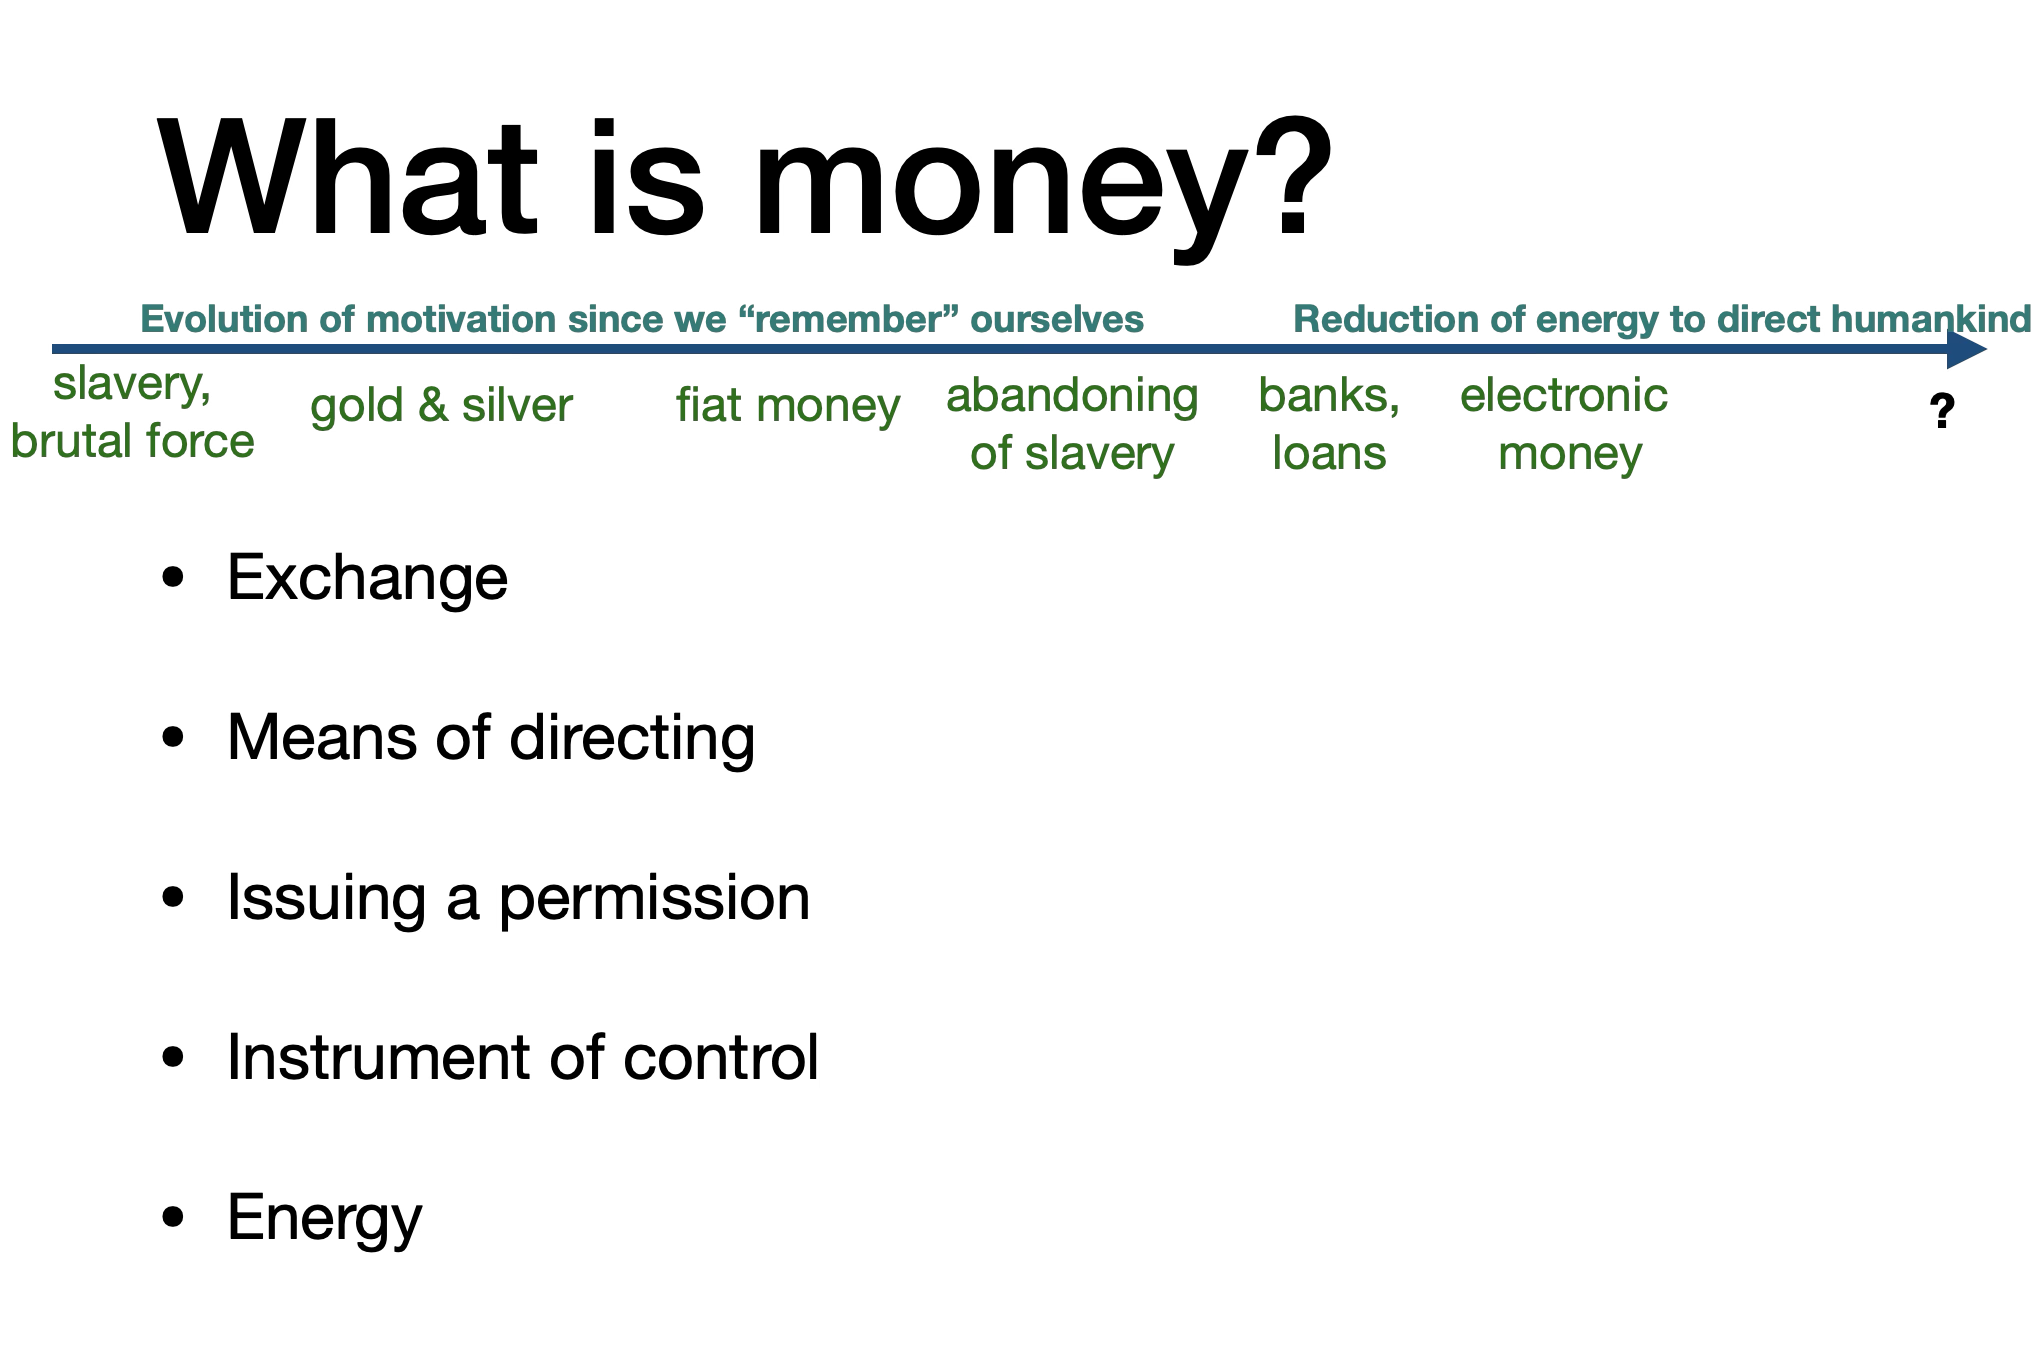
\includegraphics[width=0.75\textwidth]{fig/what_is_money.png}
    \caption{What is money? From tool to master---the transformation of money's role}
    \label{fig:money_nature}
\end{figure}

% ==================== PART 2 CONTINUED ====================

\subsubsection{Industrial Revolution (1750 CE)}

Mechanization brought:
\begin{itemize}
    \item[$+$] Unprecedented productivity, scientific progress, life expectancy gains
    \item[$-$] Humans as interchangeable machine parts
    \item[$-$] Disconnection from nature, craft, and meaningful work
    \item[$-$] Urbanization and atomization (community dissolution)
    \item[$-$] Environmental destruction at scale
\end{itemize}

\subsubsection{Financialization and Bretton Woods Collapse (1971 CE)}

Nixon's removal of gold standard \citep{brettonwoods1971} enabled:
\begin{itemize}
    \item Unlimited fiat currency creation
    \item Debt-based economy (money created as debt)
    \item Financial sector dominance over productive economy
    \item Wealth creation through speculation rather than production
\end{itemize}

\subsubsection{Digital Revolution and Attention Capture (2000-2025 CE)}

The internet and smartphones enabled:
\begin{itemize}
    \item[$+$] Information democratization, global connectivity, collaboration
    \item[$-$] Algorithmic manipulation at unprecedented scale
    \item[$-$] Attention as commodity, consciousness as resource
    \item[$-$] Filter bubbles, polarization, reality fragmentation
    \item[$-$] Automation of human connection (social media replacing embodied community)
\end{itemize}

\begin{figure}[H]
    \centering
    \includegraphics[width=0.9\textwidth]{fig/digitization_and_inequality.png}
    \caption{Digitization and inequality: the correlation between technological advancement and wealth concentration}
    \label{fig:digitization_inequality}
\end{figure}

\subsection{The Value Pumping Mechanism}

A critical dynamic of modern SYSTEM is what we call \textbf{value pumping}---the systematic extraction of value from the many to the few, mediated by technology and finance.

\begin{figure}[H]
    \centering
    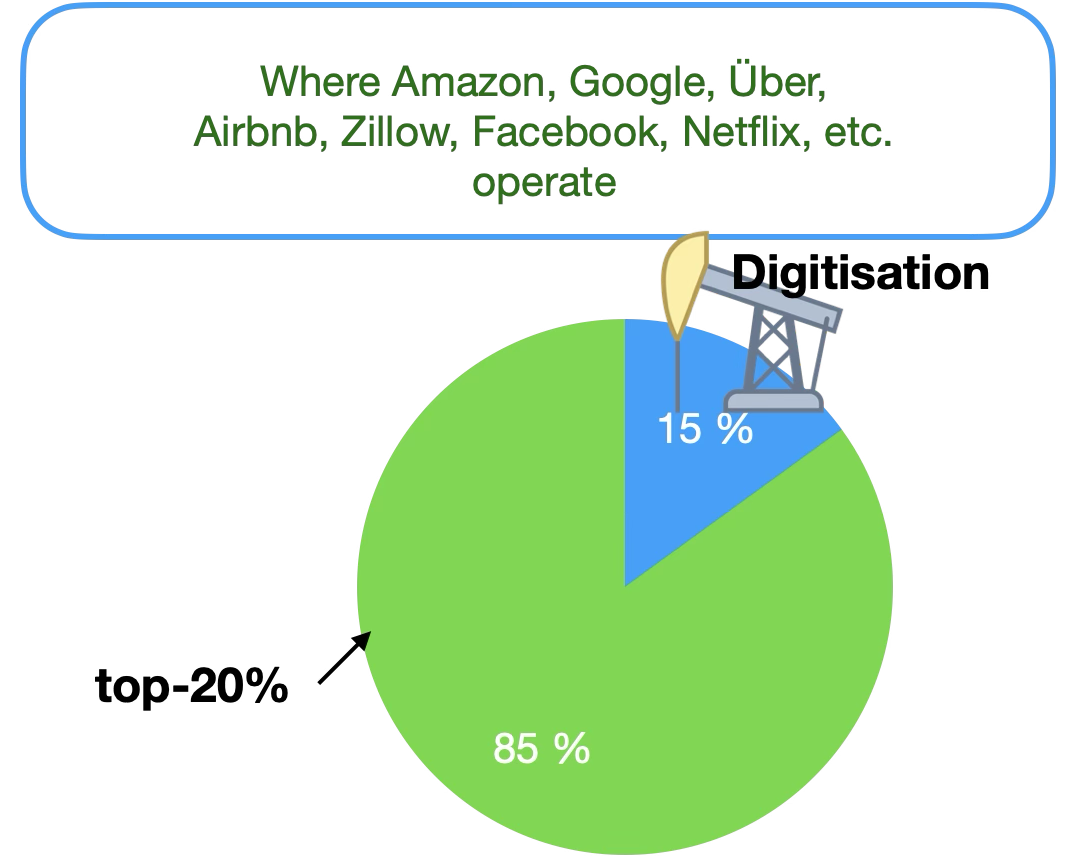
\includegraphics[width=0.85\textwidth]{fig/digitization_and_inequality_pumping_value.png}
    \caption{The value pumping mechanism: how digitization enables systematic wealth extraction}
    \label{fig:value_pump}
\end{figure}

The mechanism works as follows:

\begin{enumerate}
    \item \textbf{Platform mediation:} Technology platforms insert themselves between producers and consumers
    
    \item \textbf{Data extraction:} Platforms harvest user data (attention, preferences, behavior)
    
    \item \textbf{Algorithmic optimization:} Data used to optimize for platform goals (engagement, revenue)
    
    \item \textbf{Value capture:} Platform captures disproportionate share of value created by users/producers
    
    \item \textbf{Network effects:} Winner-take-all dynamics concentrate power in few platforms
    
    \item \textbf{Reinvestment:} Captured value used to strengthen position (acquisitions, lobbying, infrastructure)
\end{enumerate}

\begin{figure}[H]
    \centering
    \begin{subfigure}[b]{0.32\textwidth}
        \includegraphics[width=\textwidth]{fig/digitization_and_inequality_pumping_value_example_part1.png}
        \caption{Stage 1: Platform Entry}
    \end{subfigure}
    \hfill
    \begin{subfigure}[b]{0.32\textwidth}
        \includegraphics[width=\textwidth]{fig/digitization_and_inequality_pumping_value_example_part2.png}
        \caption{Stage 2: Value Capture}
    \end{subfigure}
    \hfill
    \begin{subfigure}[b]{0.32\textwidth}
        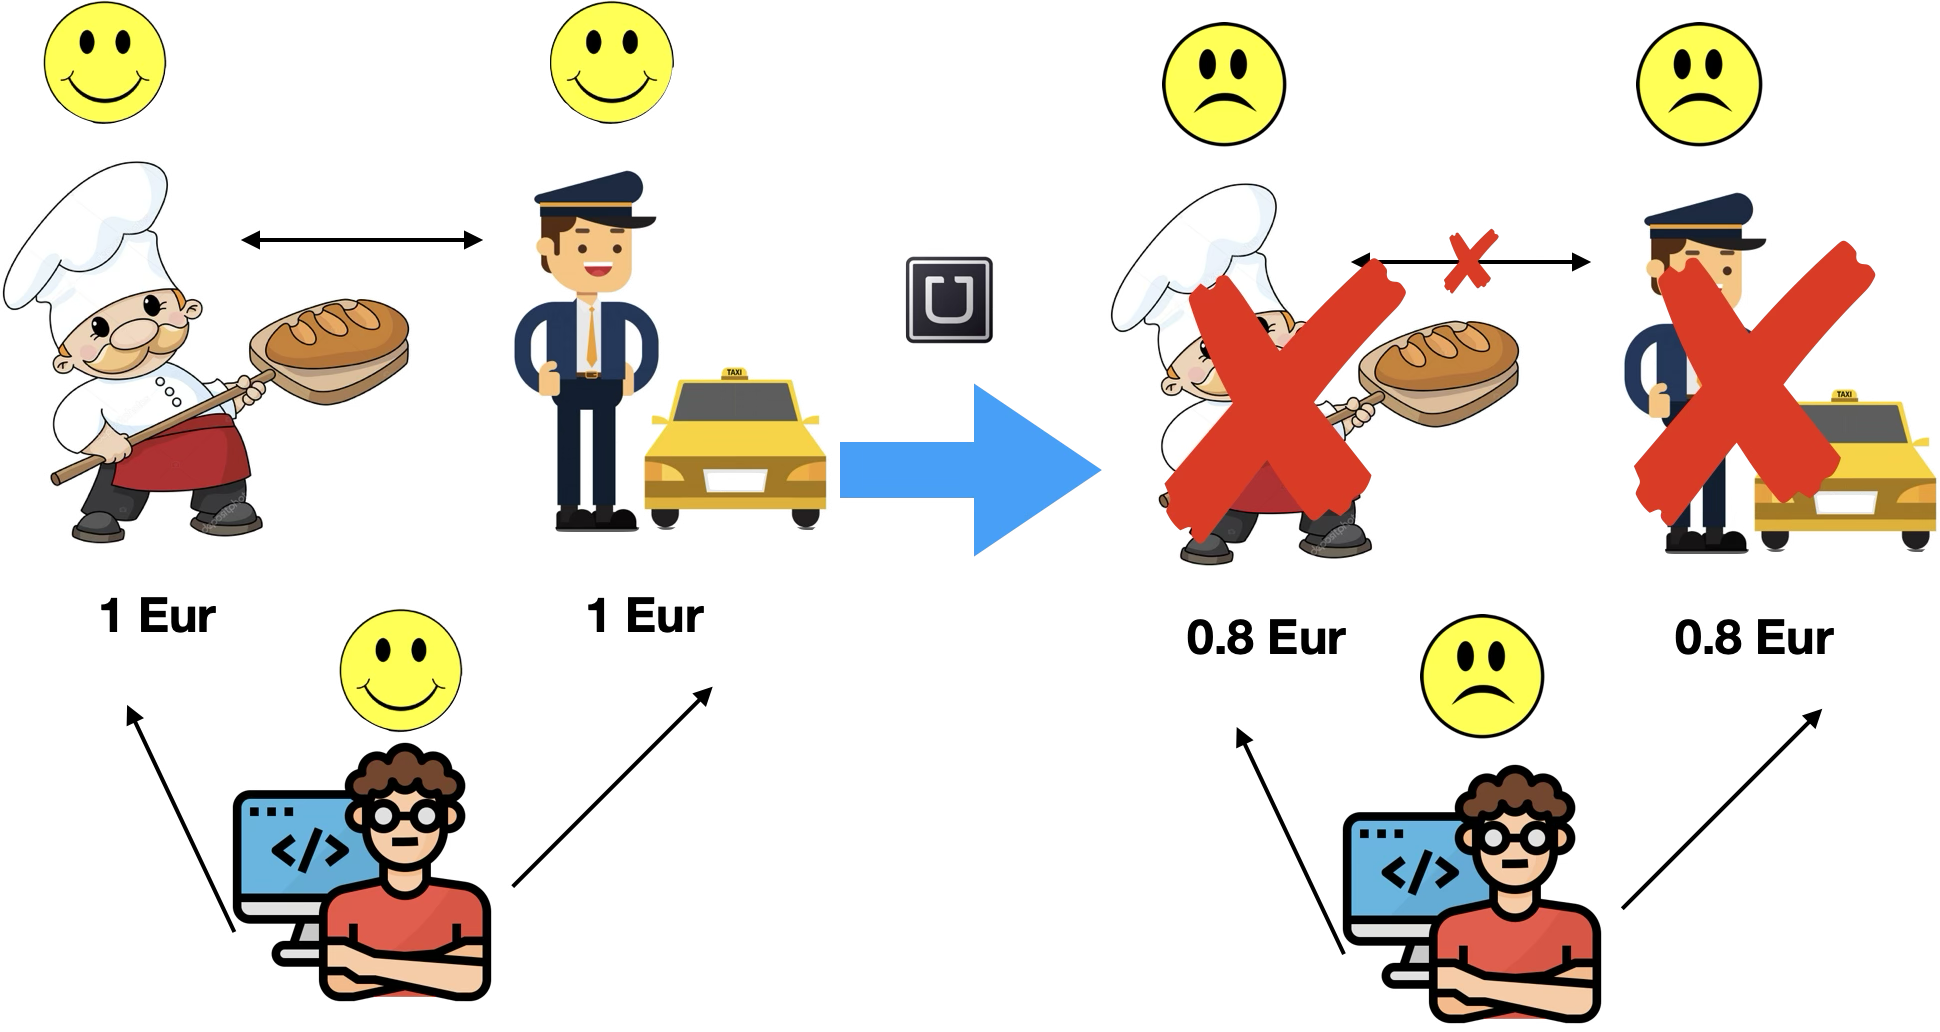
\includegraphics[width=\textwidth]{fig/digitization_and_inequality_pumping_value_example_part3.png}
        \caption{Stage 3: Concentration}
    \end{subfigure}
    \caption{Value pumping example: The three stages of platform-mediated extraction}
    \label{fig:pump_stages}
\end{figure}

Examples:
\begin{itemize}
    \item \textbf{Uber:} Captures 25-30\% of every ride. Drivers provide car, labor, maintenance. Uber provides software and brand. Who captures more value?
    
    \item \textbf{Amazon:} Third-party sellers do the work (sourcing, fulfillment, risk). Amazon charges fees, harvests data, then competes with successful products using that data.
    
    \item \textbf{Facebook/Instagram:} Users create all content. Platform provides distribution and captures advertising revenue. Users get nothing except ``exposure.''
    
    \item \textbf{Airbnb:} Hosts provide property, cleaning, hospitality. Airbnb captures 15-20\% for software platform. Hosts bear all risk.
\end{itemize}

This is extraction at scale, automated and invisible. Traditional landlords were at least visible oppressors. Digital platforms extract while maintaining the illusion of mutual benefit (``we're just connecting people!'').

\subsection{Where Is Humanity Going?}

Given current trajectories, we can project forward. The question ``where is humanity going?'' has multiple possible answers depending on whether we remain on current path or make conscious corrections.

\begin{figure}[H]
    \centering
    \includegraphics[width=0.9\textwidth]{fig/human_evolution.png}
    \caption{Human evolution: from biological to technological to conscious?}
    \label{fig:human_evolution}
\end{figure}

\subsubsection{Trajectory 1: Continued Fall (Business as Usual)}

If current patterns continue uninterrupted:
\begin{itemize}
    \item \textbf{2030-2040:} Climate tipping points crossed (Arctic ice, Amazon rainforest, permafrost)
    \item \textbf{2040-2050:} Mass migration (1-2 billion climate refugees), resource wars
    \item \textbf{2050-2070:} Ecosystem collapse, food system failure, societal breakdown
    \item \textbf{2070-2100:} Potential human population collapse from 10B to 1-2B
\end{itemize}

This is not alarmism but extrapolation. Current trajectory is \textit{unsustainable} by definition---it cannot continue indefinitely.

\subsubsection{Trajectory 2: Techno-Dystopia}

Alternatively, technological ``solutions'' without consciousness evolution:
\begin{itemize}
    \item Surveillance capitalism perfected (everyone tracked, predicted, controlled)
    \item Genetic engineering creates biological class hierarchy
    \item AI automation creates permanent unemployability for billions
    \item Virtual reality as opiate (real world unlivable, everyone in pods)
    \item Authoritarian control necessary to manage scarcity and instability
\end{itemize}

This is SYSTEM achieving ``stability'' through total control---a stable state, but one of maximal dehumanization. Think \textit{Brave New World} meets \textit{1984}, powered by AI.

\subsubsection{Trajectory 3: Conscious Evolution}

The alternative we advocate:
\begin{itemize}
    \item Mass awakening to SYSTEM patterns and conscious refusal to participate
    \item Development of alternative economic structures (PEMY-type models)
    \item Technology used to enhance consciousness rather than capture it
    \item Education reformed to develop wisdom alongside knowledge
    \item Governance structures redesigned for long-term, multi-stakeholder benefit
\end{itemize}

This is not utopian fantasy but practical necessity. Either consciousness evolves, or civilization collapses. There is no stable middle ground.

\subsection{The Adolescent Humanity Metaphor}

A useful framing: Humanity is currently an \textbf{adolescent}---powerful but unwise, full of energy but lacking discipline, technically capable but ethically underdeveloped.

\begin{itemize}
    \item \textbf{Like teenagers:} We can drive cars (technology) but crash them (climate change, nuclear weapons)
    \item \textbf{Like teenagers:} We think we know everything but are profoundly ignorant of consequences
    \item \textbf{Like teenagers:} We prioritize short-term pleasure over long-term wellbeing
    \item \textbf{Like teenagers:} We rebel against wisdom (``don't tell me what to do!'')
    \item \textbf{Like teenagers:} We're obsessed with status and fitting in with peers
\end{itemize}

The question: Will humanity mature into adulthood, or self-destruct in adolescence?

Adulthood means:
\begin{itemize}
    \item Taking responsibility for consequences
    \item Delaying gratification for greater future good
    \item Integrating wisdom with capability
    \item Caring for those dependent on us (future generations, ecosystems)
    \item Conscious choice rather than reactive impulse
\end{itemize}

\section{Case Studies: SYSTEM in Practice}

To make our analysis concrete, we examine specific instances where SYSTEM dynamics play out with particular clarity.

\subsection{Case Study 1: The Gazprom-Europe Relationship}

\begin{figure}[H]
    \centering
    
\includegraphics[width=0.4\textwidth]{fig/gazprom_logo.jpeg}
    \caption{Gazprom: A case study in energy dependence and geopolitical leverage}
    \label{fig:gazprom}
\end{figure}

Europe's dependence on Russian natural gas (via Gazprom) illustrates multiple SYSTEM patterns:

\begin{itemize}
    \item \textbf{Short-term optimization:} Cheap gas prioritized over energy independence/diversification
    \item \textbf{Institutional capture:} Former politicians join Gazprom boards (e.g., Gerhard Schröder)
    \item \textbf{Collective delusion:} Belief that economic interdependence prevents conflict (disconfirmed 2022)
    \item \textbf{Path dependence:} Infrastructure lock-in makes rapid transition costly
    \item \textbf{Strategic blindness:} Ignoring warnings for years because acknowledging risk requires uncomfortable change
\end{itemize}

The 2022 invasion of Ukraine revealed the fragility of this arrangement. Europe had traded autonomy for convenience, consciousness for unconscious drift.

\subsection{Case Study 2: Social Media and the Pretending-vs-Being Gap}

\begin{figure}[H]
    \centering
    
\includegraphics[width=0.85\textwidth]{fig/socialmedia_illustration_pr-pretending_vs_being.png}
    \caption{Social media: The widening gap between pretending and being}
    \label{fig:social_media_gap}
\end{figure}

Social media creates systematic incentives for \textbf{pretending} over \textbf{being}:

\begin{itemize}
    \item \textbf{Performance pressure:} Life becomes content. Experiences valued by shareability not intrinsic meaning.
    \item \textbf{Selective presentation:} Highlight reel vs. reality. Everyone else seems happier/successful/beautiful.
    \item \textbf{Validation addiction:} Likes/followers become proxy for self-worth. External metric replaces internal knowing.
    \item \textbf{Comparison trap:} Constant exposure to curated perfection breeds inadequacy.
    \item \textbf{Authenticity penalty:} Vulnerable honesty gets less engagement than polished performance.
\end{itemize}

Result: A generation increasingly disconnected from their own experience, performing identity rather than living it. This is dehumanization at the level of selfhood---you become the brand you project rather than the consciousness you are.

The feedback loop:
\begin{equation}
\text{Post performance} \to \text{Get validation} \to \text{Crave more} \to \text{Perform more} \to \text{Forget authentic self}
\end{equation}

\subsection{Case Study 3: Mark Zuckerberg and Goal-Reality Inconsistency}

\begin{figure}[H]
    \centering
    \includegraphics[width=0.75\textwidth]{fig/mark_zuckerberg_inconsistency_goal_reality.png}
    \caption{The Zuckerberg paradox: stated goals vs. actual outcomes}
    \label{fig:zuckerberg}
\end{figure}

Facebook's stated mission: ``Bring the world closer together.''

Actual effects:
\begin{itemize}
    \item Polarization increased (filter bubbles, rage engagement)
    \item Democracy undermined (disinformation, election interference)
    \item Mental health declined (especially teen girls)
    \item Attention fragmented (constant distraction)
    \item Privacy eroded (surveillance business model)
\end{itemize}

This is not hypocrisy---it's \textbf{unconsciousness}. Zuckerberg may genuinely believe the mission. But the \textit{system he built} optimizes for engagement (ad revenue), not connection. The algorithm doesn't care about truth or wellbeing; it cares about clicks.

Key insight: \textbf{Stated goals vs. optimization functions}. What you \textit{say} you're doing vs. what you're actually \textit{optimizing for}. When these diverge, the optimization function wins every time.

This pattern repeats across SYSTEM:
\begin{itemize}
    \item Politicians: ``Serve the people'' / Optimize for: Re-election (hence donor appeasement)
    \item Corporations: ``Create value'' / Optimize for: Shareholder returns (hence extraction)
    \item Universities: ``Pursue truth'' / Optimize for: Rankings and grants (hence conformity)
    \item Media: ``Inform public'' / Optimize for: Attention (hence sensationalism)
\end{itemize}

\subsection{Case Study 4: Telegram and Platform Governance}

\begin{figure}[H]
    \centering
    
\includegraphics[width=0.3\textwidth]{fig/telegram_logo.jpeg}
    \caption{Telegram: Alternative platform or different flavor of the same pattern?}
    \label{fig:telegram}
\end{figure}

Telegram positions itself as privacy-focused alternative to mainstream platforms. But analysis reveals similar SYSTEM patterns:

\begin{itemize}
    \item \textbf{Centralized control:} Pavel Durov has unilateral power over platform
    \item \textbf{Opaque governance:} Decision-making processes hidden
    \item \textbf{Monetization pressures:} Will inevitably face pressure to extract value from users
    \item \textbf{Savior narrative:} ``We're different'' becomes marketing, not practice
\end{itemize}

Key lesson: Changing platforms doesn't escape SYSTEM if the \textit{structure} remains the same (centralized, extractive, opacity). Need fundamentally different architecture---which is what PEMY proposes.

% ==================== PART III: SOLUTIONS ====================
\part{Solutions and Transformation}

\section{Individual Practices: Consciousness Development}

Having diagnosed SYSTEM, we now turn to solutions. Transformation must happen at two levels simultaneously: \textbf{individual} (consciousness development) and \textbf{systemic} (structural alternatives). Neither alone is sufficient.

\subsection{The Epistemological Boxing Protocol (EBP)}

From S.V.E. 0 \citep{sve0}, EBP is a practice for developing clarity and testing beliefs:

\begin{enumerate}
    \item \textbf{Make claim explicit:} State belief as falsifiable proposition
    \item \textbf{Identify assumptions:} What must be true for this belief to hold?
    \item \textbf{Find counterexamples:} Actively seek evidence against belief
    \item \textbf{Steelman opposition:} Construct strongest possible counterargument
    \item \textbf{Update or strengthen:} Modify belief based on evidence, or clarify why objections fail
\end{enumerate}

This protocol \textit{operationalizes} intellectual honesty. You literally cannot complete it while maintaining obviously false beliefs. It's like a debugger for thought.

\textbf{Example application:}
\begin{itemize}
    \item \textit{Belief:} ``I need to work 60 hours/week to be successful.''
    \item \textit{Assumptions:} Success = wealth/status. More hours = more output. Others are doing this.
    \item \textit{Counterexamples:} Many successful people work 40 hours or less. Research shows diminishing returns after 40 hours. Burnout reduces long-term productivity.
    \item \textit{Steelman opposition:} Perhaps success isn't what I thought. Maybe I'm optimizing for the wrong metric. Maybe I'm running a program inherited from SYSTEM rather than choosing consciously.
    \item \textit{Update:} Redefine success. Experiment with working less. Track actual productivity vs. hours.
\end{itemize}

\subsection{The Structured Introspection Protocol (SIP)}

Also from S.V.E. 0, SIP is a daily practice for developing self-awareness:

\begin{enumerate}
    \item \textbf{Morning calibration (10 min):}
    \begin{itemize}
        \item What is my current state? (physical, emotional, mental)
        \item What patterns am I running? (habits, scripts, defaults)
        \item What do I genuinely want today? (not what I ``should'' want)
    \end{itemize}
    
    \item \textbf{Midday checkpoint (5 min):}
    \begin{itemize}
        \item Am I present or on autopilot?
        \item Am I acting from consciousness or pattern?
        \item What needs adjusting?
    \end{itemize}
    
    \item \textbf{Evening review (15 min):}
    \begin{itemize}
        \item What moments was I most/least conscious?
        \item What patterns repeated?
        \item What did I learn about myself?
        \item What experiment will I run tomorrow?
    \end{itemize}
\end{enumerate}

This is not navel-gazing---it's \textbf{empirical self-study}. You're treating yourself as a system to understand, debug, and optimize. Over time, you develop the capacity to see your own unconscious patterns \textit{as they run}, which is the first step to changing them.

\subsection{Practices for Deconditioning}

SYSTEM operates through conditioning---learned patterns that run automatically. Deconditioning means:

\subsubsection{Attention Reclamation}
\begin{itemize}
    \item Digital detox periods (no screens for 24-72 hours)
    \item Notification abolition (nothing interrupts you without permission)
    \item Monotasking practice (one thing at a time, fully present)
    \item Boredom tolerance (sit without entertainment, observe what arises)
\end{itemize}

\subsubsection{Consumption Consciousness}
\begin{itemize}
    \item Track what you consume (food, media, products) for one week
    \item For each consumption, ask: ``Why did I do this? Was it conscious choice or automatic response?''
    \item Experiment: Go one week only consuming what you \textit{intentionally} choose (no impulsive anything)
    \item Observe: How much of your life is actually chosen vs. programmed?
\end{itemize}

\subsubsection{Social Reality Testing}
\begin{itemize}
    \item Identify one belief everyone around you shares
    \item Research counterarguments seriously (even if it feels wrong)
    \item Talk to people who believe differently (not to convert, but to understand)
    \item Notice: How much of what you ``know'' is actually inherited assumption?
\end{itemize}

\subsubsection{Relationship to Money}
\begin{itemize}
    \item Write your money story: How did you learn about money? What do you believe about it?
    \item Track every financial decision for one month: Necessary vs. optional? Conscious vs. automatic?
    \item Experiment: Go one month spending only on what serves your genuine values (not should, not status)
    \item Reflect: Is money serving you, or are you serving money?
\end{itemize}

\subsection{Building Antifragility}

From Taleb \citep{taleb2012antifragile}, antifragility means \textit{gaining from disorder}. For individuals:

\begin{itemize}
    \item \textbf{Skills over credentials:} Can you actually do things, or just show certificates?
    \item \textbf{Multiple income streams:} Don't depend on one employer/client
    \item \textbf{Debt minimization:} The less you owe, the freer you are
    \item \textbf{Community over institutions:} Strong local relationships more robust than distant institutions
    \item \textbf{Optionality:} Maintain multiple paths forward, don't lock into one
\end{itemize}

These are not just practical tips---they're \textbf{structural resistance to SYSTEM}. The more antifragile you are, the less leverage SYSTEM has over you.

\section{The PEMY Model: Systemic Alternative to Extractive Capitalism}

Individual consciousness development is necessary but not sufficient. We also need \textbf{alternative structures} that embody different principles. Enter PEMY.

\subsection{What is PEMY?}

\textbf{PEMY} = \textbf{P}eople + \textbf{E}nvironment + \textbf{M}oney + \textbf{Y}ou

It's a business model where:
\begin{itemize}
    \item \textbf{People:} All workers are owners (shareholders)
    \item \textbf{Environment:} Ecological health is explicit goal, not externality
    \item \textbf{Money:} Profits distributed to stakeholders, not extracted to distant shareholders
    \item \textbf{You:} Every participant has voice, vote, and agency in governance
\end{itemize}

\begin{figure}[H]
    \centering
    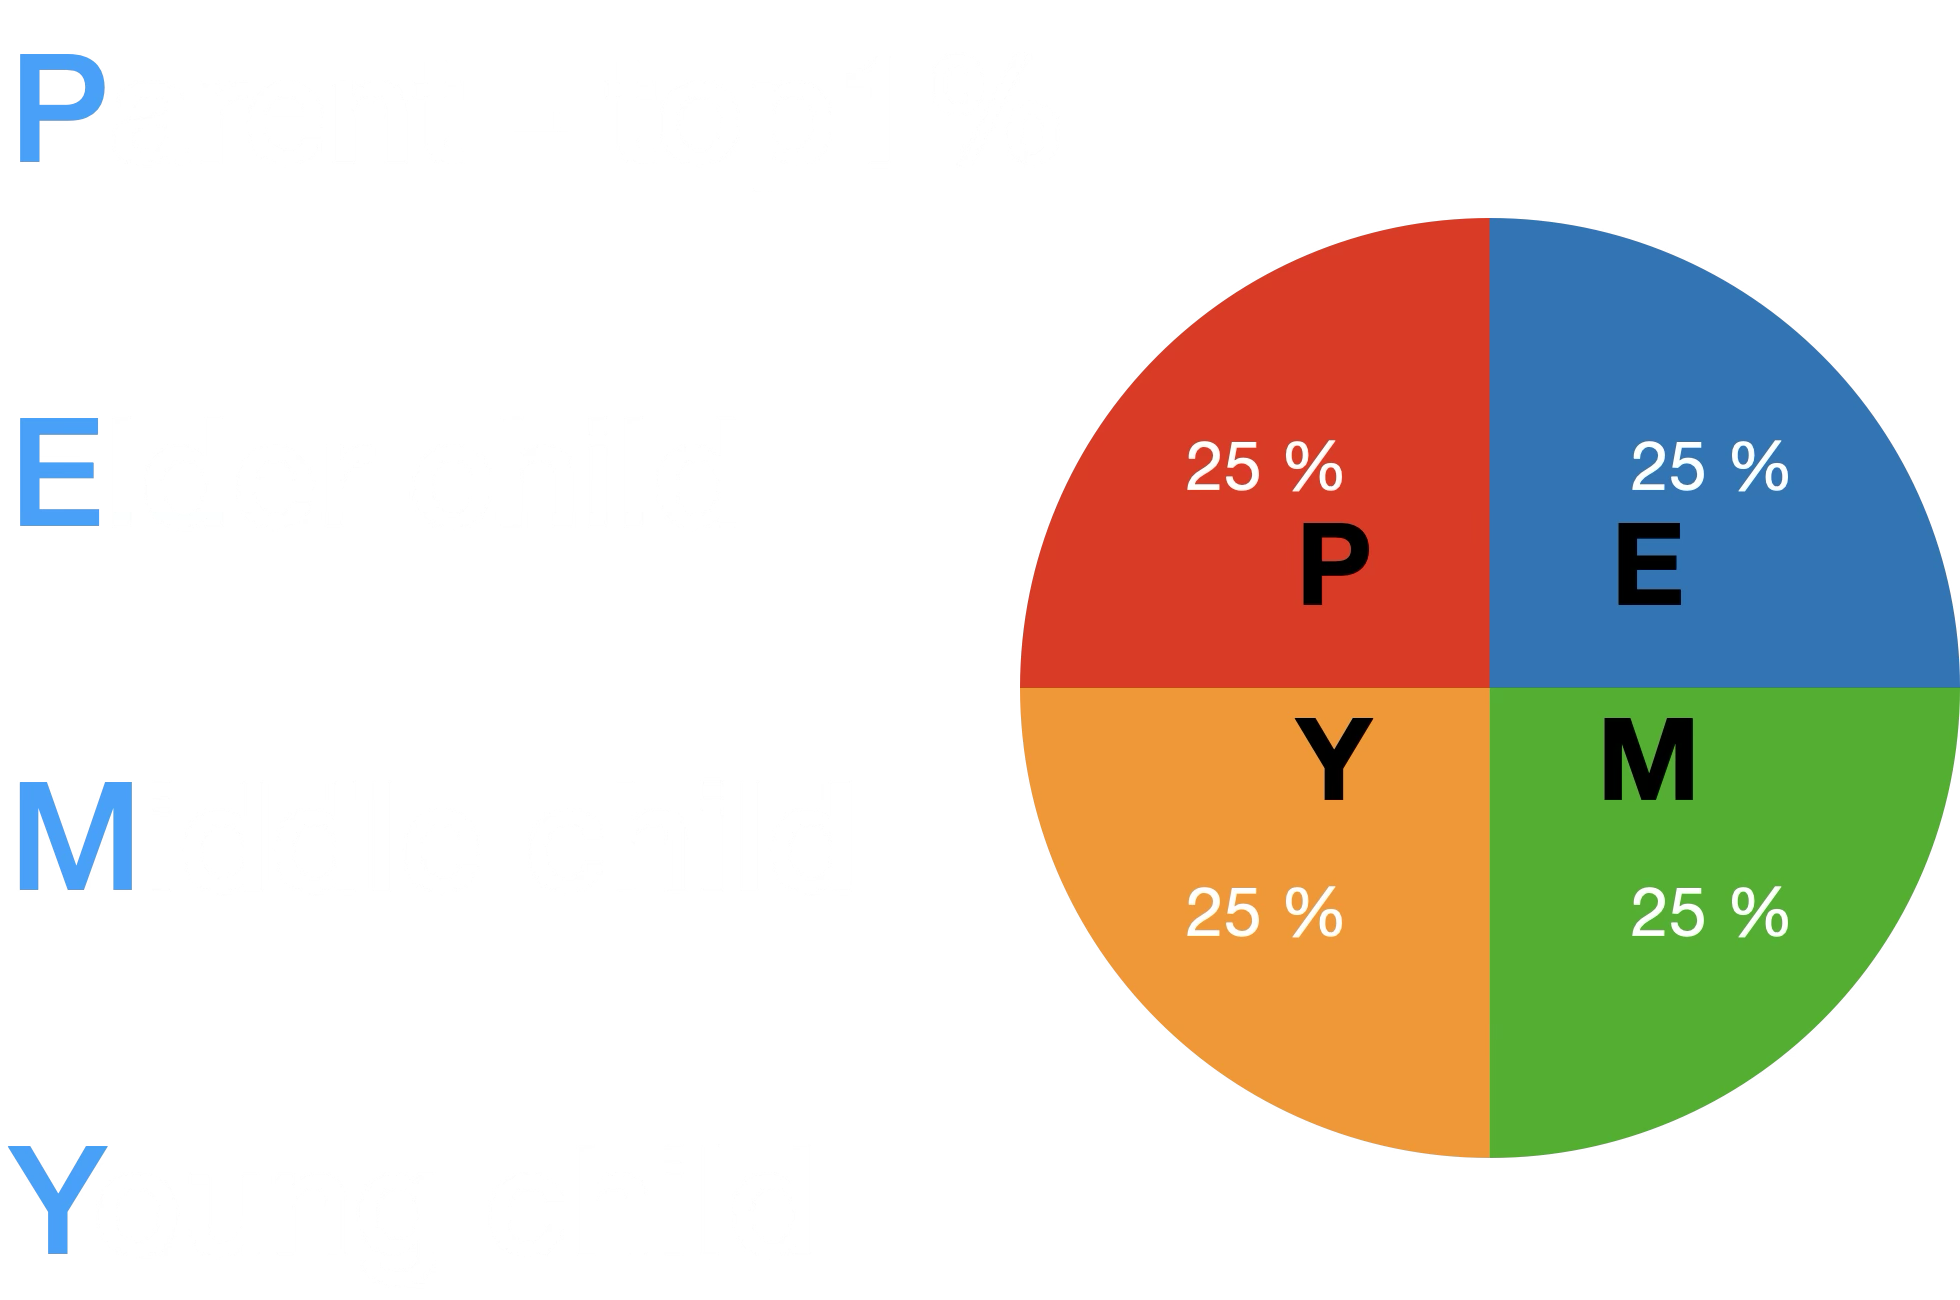
\includegraphics[width=0.9\textwidth]{fig/pemy_part_1.png}
    \caption{PEMY Part 1: The foundational structure of stakeholder capitalism}
    \label{fig:pemy_1}
\end{figure}

Think of PEMY as \textbf{correcting the bug} in traditional capitalism: the concentration of ownership and extraction of value. It retains:
\begin{itemize}
    \item Market competition
    \item Innovation incentives
    \item Profit motive
    \item Private ownership
\end{itemize}

But distributes them differently:
\begin{itemize}
    \item Ownership: Distributed across stakeholders, not concentrated in distant investors
    \item Profits: Reinvested or shared, not extracted
    \item Decision-making: Democratic/participatory, not dictatorial
    \item Goals: Multi-capital optimization, not single-metric (profit) maximization
\end{itemize}

\subsection{PEMY Architecture}

\begin{figure}[H]
    \centering
    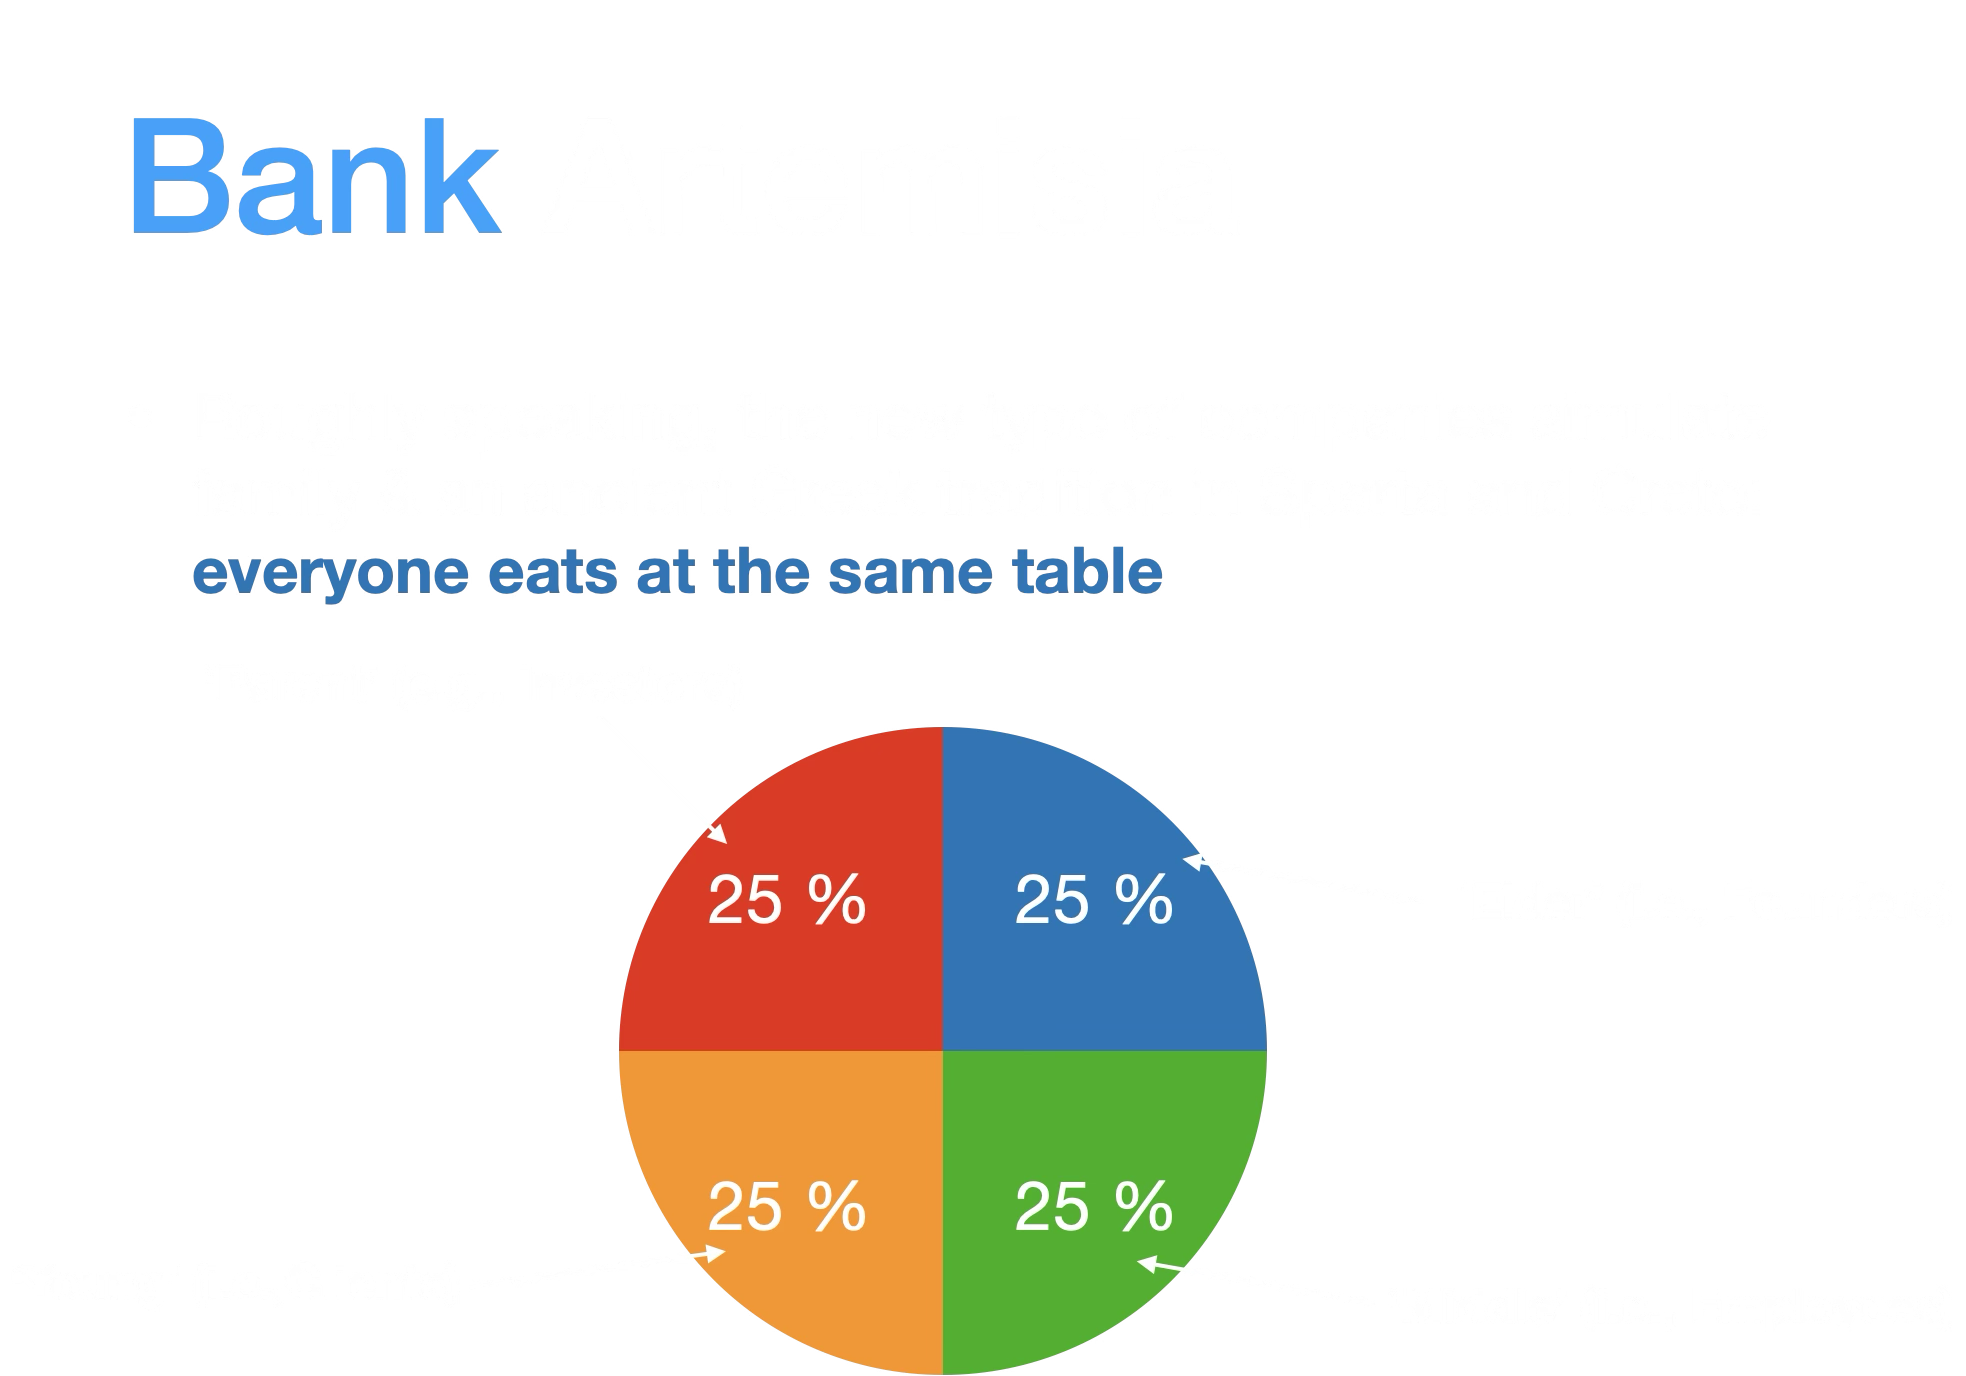
\includegraphics[width=0.9\textwidth]{fig/pemy_part_2.png}
    \caption{PEMY Part 2: Governance and decision-making structures}
    \label{fig:pemy_2}
\end{figure}

\subsubsection{Ownership Structure}

Shares distributed across stakeholder groups:
\begin{itemize}
    \item \textbf{Workers (40-50\%):} Those doing the actual work
    \item \textbf{Community (20-30\%):} Local community affected by operations
    \item \textbf{Customers (10-20\%):} Those using products/services
    \item \textbf{Founders/Investors (20-30\%):} Those who initiated and risked capital
    \item \textbf{Future Fund (5-10\%):} Reserved for environmental restoration and next generation
\end{itemize}

Exact ratios can vary by industry and context, but principle remains: \textbf{broad distribution} rather than concentration.

\subsubsection{Governance Principles}

\begin{enumerate}
    \item \textbf{One person, one vote} (or weighted by tenure/contribution, but capped)
    \\
    \textit{Not} one dollar, one vote
    
    \item \textbf{Supermajority for major decisions}
    \\
    Changes requiring 60-70\% agreement across \textit{all} stakeholder groups
    
    \item \textbf{Transparency by default}
    \\
    All financials, decisions, and discussions open to stakeholders
    
    \item \textbf{Limited terms for leadership}
    \\
    Prevent emergence of entrenched elite
    
    \item \textbf{Conflict resolution protocols}
    \\
    Structured processes for handling disagreements (like EBP for organizations)
\end{enumerate}

\begin{figure}[H]
    \centering
    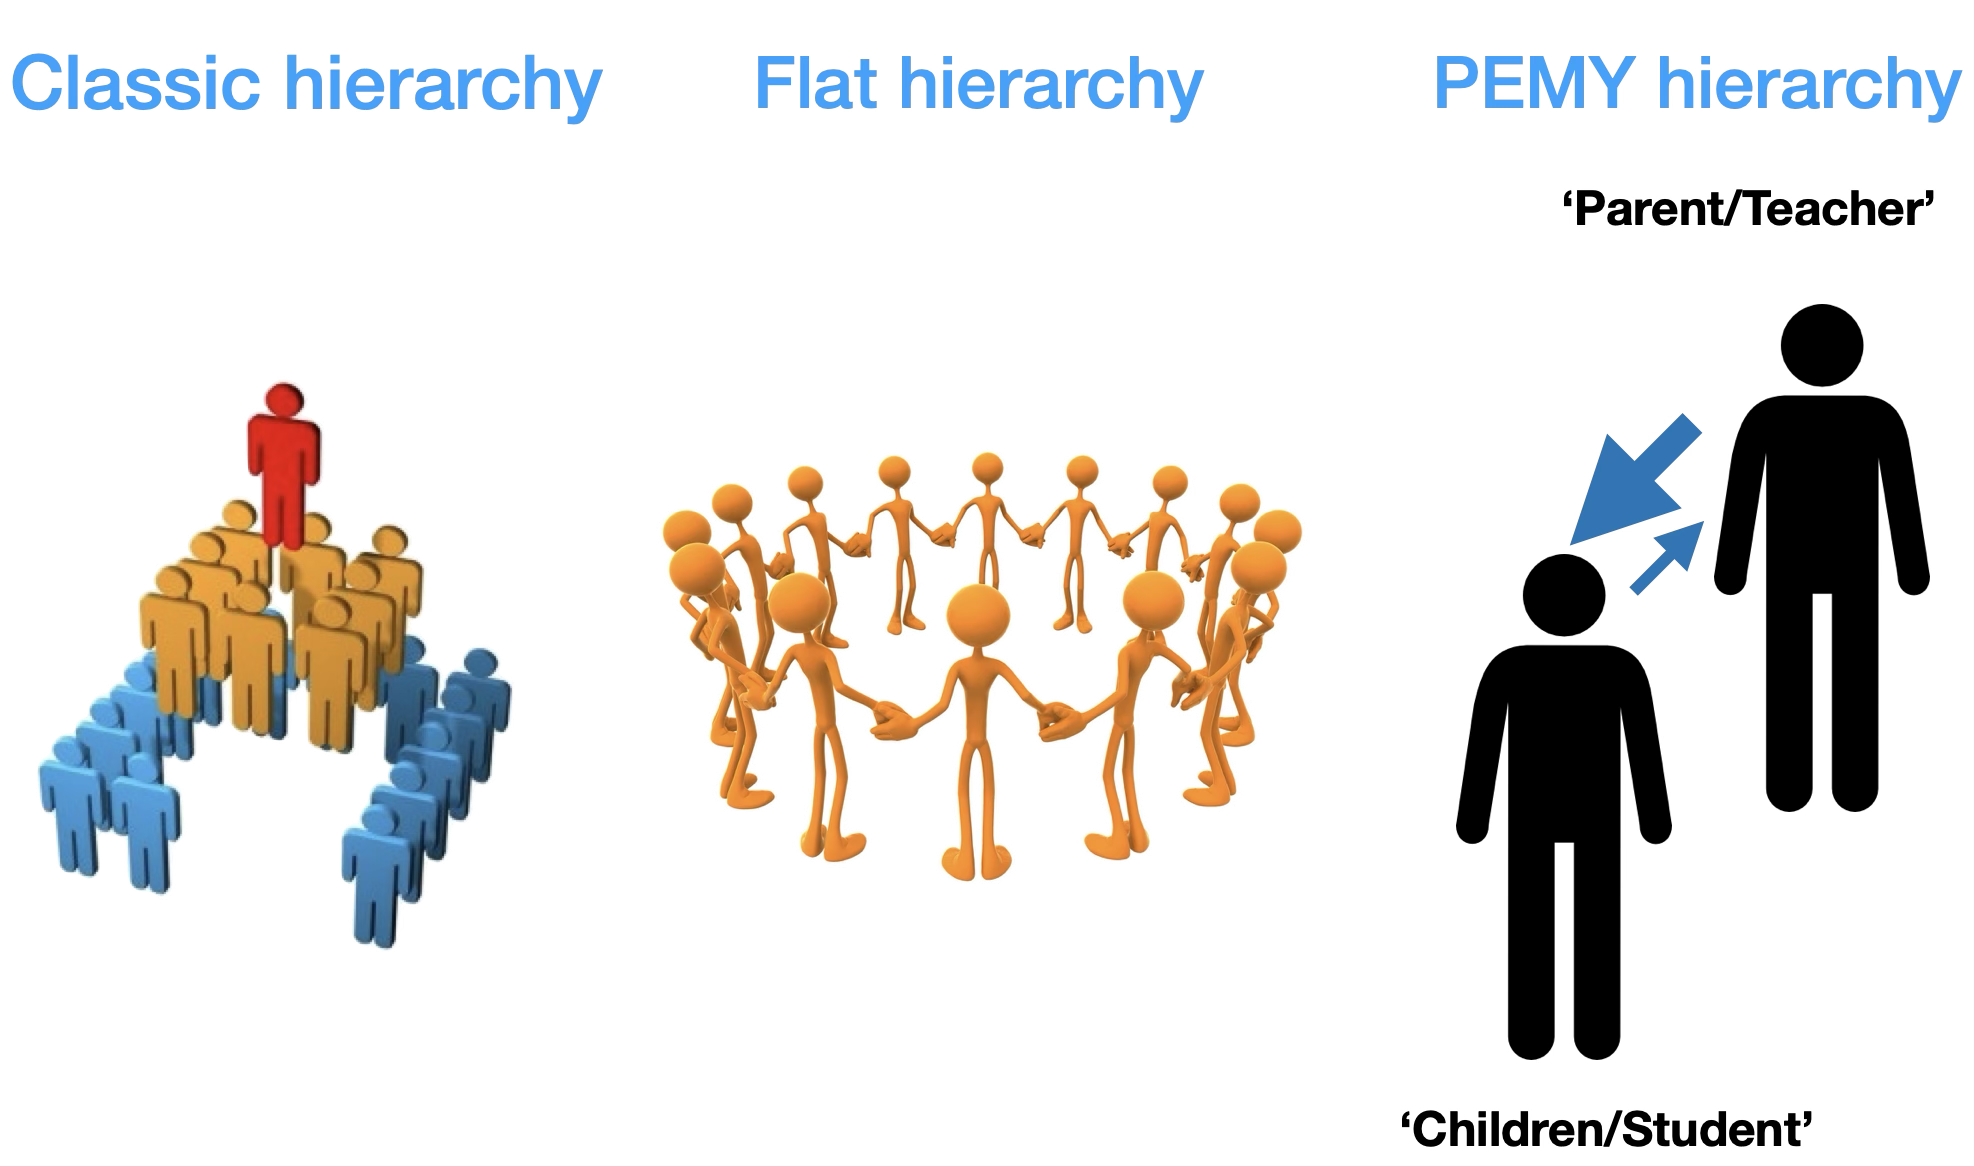
\includegraphics[width=0.9\textwidth]{fig/pemy_part_3_hierarchy.png}
    \caption{PEMY Part 3: Organizational hierarchy---flat but not structureless}
    \label{fig:pemy_3}
\end{figure}

\subsection{Comparison: Type 1 vs Type 2 (PEMY) Firms}

\begin{figure}[H]
    \centering
    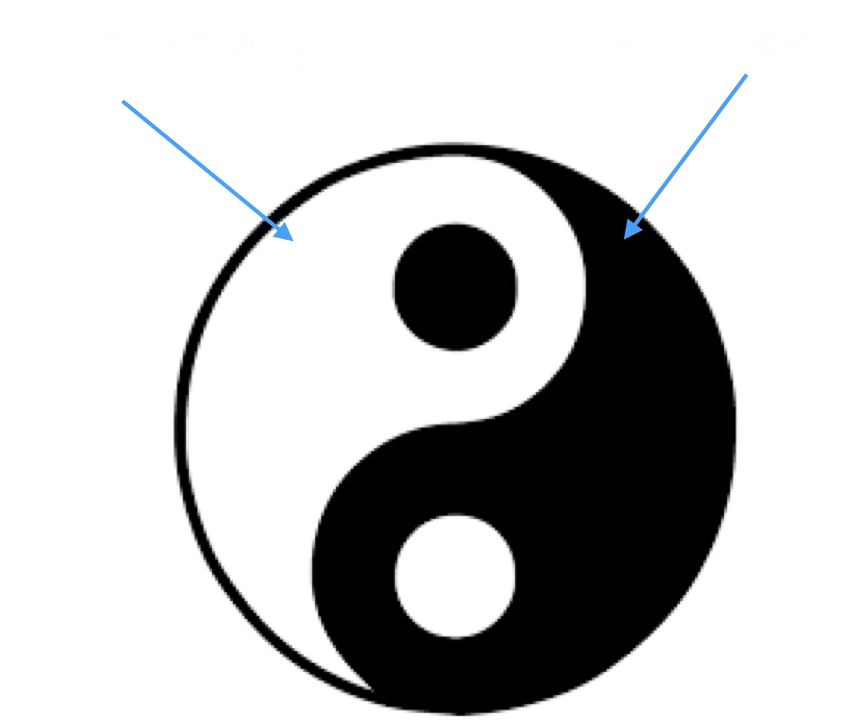
\includegraphics[width=0.85\textwidth]{fig/inyan_uber_type1_type2_PEMY.png}
    \caption{Yin-Yang of economic models: Type 1 (extractive) vs Type 2 (PEMY) firms as complementary forces}
    \label{fig:type_comparison}
\end{figure}

\begin{table}[H]
\centering
\caption{Type 1 (Traditional) vs Type 2 (PEMY) Firm Comparison}
\begin{tabularx}{\textwidth}{lXX}
\toprule
\textbf{Dimension} & \textbf{Type 1 (Extractive)} & \textbf{Type 2 (PEMY)} \\
\midrule
Ownership & Concentrated (shareholders) & Distributed (stakeholders) \\
Primary goal & Maximize shareholder value & Optimize multi-capital wellbeing \\
Workers & Cost to minimize & Partners to develop \\
Environment & Externality to ignore & Capital to preserve \\
Community & Irrelevant & Stakeholder with voice \\
Time horizon & Quarterly results & Generational sustainability \\
Transparency & Minimal (trade secrets) & Maximal (within stakeholders) \\
Governance & Top-down hierarchy & Participatory democracy \\
Innovation & For competitive advantage & For collective benefit \\
Profits & Extracted to owners & Reinvested or shared \\
\bottomrule
\end{tabularx}
\label{tab:type_comparison}
\end{table}

\subsection{How PEMY Addresses SYSTEM Pathologies}

Each feature of PEMY directly counters a SYSTEM dynamic:

\begin{itemize}
    \item \textbf{Distributed ownership} $\to$ Prevents wealth concentration and extraction
    \item \textbf{Multi-capital accounting} $\to$ Makes externalities internal (can't ignore environmental/social costs)
    \item \textbf{Democratic governance} $\to$ Distributes power, prevents oligarchy
    \item \textbf{Long-term orientation} $\to$ Aligns with sustainability rather than quarterly pump
    \item \textbf{Transparency} $\to$ Makes unconscious patterns visible
    \item \textbf{Community stake} $\to$ Connects firm to place and people
\end{itemize}

PEMY is SYSTEM's antithesis: conscious where SYSTEM is unconscious, regenerative where SYSTEM is extractive, integrative where SYSTEM is fragmentary.

\subsection{Practical Objections and Responses}

\subsubsection{``This will be less efficient/profitable''}

\textit{Response:} Efficiency for what goal? If the goal is sustainable human flourishing (not quarterly shareholder returns), PEMY may be \textit{more} efficient.

Evidence:
\begin{itemize}
    \item Mondragon (Spain): 80,000+ worker-owners, survived 2008 crisis better than traditional firms
    \item John Lewis (UK): Employee-owned, consistently high satisfaction and profitability
    \item Cooperatives globally: Lower failure rate than traditional startups
\end{itemize}

When workers own the enterprise, they're intrinsically motivated---no need for expensive surveillance and incentive engineering.

\subsubsection{``People are too selfish---this requires unrealistic altruism''}

\textit{Response:} PEMY doesn't require altruism---it \textbf{aligns self-interest with collective interest} through ownership structure.

When your wellbeing is tied to the company's wellbeing, and the company's wellbeing is tied to community and environment, you're incentivized to care. It's enlightened self-interest, not sacrifice.

Traditional capitalism \textit{mis-aligns} interests, creating adversarial relationships between owners/workers/customers. PEMY \textit{re-aligns} them.

\subsubsection{``This is just socialism/communism rebranded''}

\textit{Response:} No. PEMY retains:
\begin{itemize}
    \item Private ownership (distributed, not state-owned)
    \item Market competition (PEMY firms compete with each other and traditional firms)
    \item Profit motive (but distributed, not extracted)
    \item Innovation incentives (workers benefit from improvements)
\end{itemize}

It's \textit{capitalism with corrected incentives}, not its abolition. Think: ``capitalism without the bug of ownership concentration.''

\subsubsection{``How do we transition without destroying the existing economy?''}

\textit{Response:} Gradual, parallel development. Create PEMY entities alongside traditional ones and let them compete in markets. Over time, if PEMY proves superior in resilience and satisfaction, it gains market share organically.

No revolution required---just better alternatives that outcompete on relevant metrics.

Legal frameworks can facilitate: tax incentives for PEMY structures, recognition as B Corps or cooperatives, preference in public contracting.

\subsubsection{``What about capital raising? VCs won't invest without control''}

\textit{Response:} True---traditional VC model is incompatible with PEMY. But alternative funding exists:
\begin{itemize}
    \item Cooperative banks / credit unions
    \item Patient capital funds (long-term investors accepting lower but stable returns)
    \item Crowdfunding from community stakeholders
    \item Revenue-based financing (investors get \% of revenue until cap, not equity control)
    \item Retained earnings (slower growth, but autonomous)
\end{itemize}

Question: Do we optimize for explosive growth with eventual capture by capital, or sustainable growth with retained autonomy?

PEMY chooses the latter. Not anti-growth, but \textit{sustainable growth}.

\subsection{Historical Precedents}

PEMY is not utopian invention but synthesis of proven models:

\begin{itemize}
    \item \textbf{Mondragon Corporation (Spain):} Worker cooperative federation, 80,000+ members, manufacturing/retail/finance/education
    
    \item \textbf{John Lewis Partnership (UK):} 80,000+ employee-owners (``Partners''), high satisfaction and service quality
    
    \item \textbf{B Corporations:} Legal status for social/environmental commitment alongside profit, 4,000+ certified globally
    
    \item \textbf{Platform Cooperatives:}
    \begin{itemize}
        \item The Drivers Cooperative (NYC): Driver-owned ride-sharing
        \item Resonate: Musician-owned streaming platform
        \item Local Food Hub: Farmer-owned food distribution
    \end{itemize}
    
    \item \textbf{Credit Unions:} Member-owned financial institutions, globally successful
\end{itemize}

These demonstrate that PEMY-like structures are not fantasy but practical reality at various scales.

\section{Transition Strategies: From Here to There}

Understanding SYSTEM and having alternatives is not enough. We need \textbf{pathways} for actual transformation.

\subsection{Multi-Level Intervention}

Change must happen simultaneously at multiple levels:

\begin{enumerate}
    \item \textbf{Individual:} Consciousness development (practices from Section 8)
    \item \textbf{Organizational:} Create/join PEMY-type structures
    \item \textbf{Community:} Build local resilience and alternatives
    \item \textbf{Cultural:} Shift narratives and collective understanding
    \item \textbf{Political:} Advocate for systemic reforms
\end{enumerate}

None alone is sufficient; together they can catalyze phase transition.

\subsection{The Dual Power Strategy}

Rather than trying to reform existing institutions (difficult, often captured), build \textbf{parallel structures} that demonstrate alternatives:

\begin{itemize}
    \item \textbf{Cooperatives} alongside corporations
    \item \textbf{Community land trusts} alongside private real estate
    \item \textbf{Mutual aid networks} alongside government welfare
    \item \textbf{Decentralized platforms} alongside Big Tech
    \item \textbf{Regenerative agriculture} alongside industrial farming
\end{itemize}

As alternatives prove viable and attractive, people migrate toward them. Eventually, old structures lose relevance and wither.

This is evolution, not revolution. Less violent, more sustainable.

\subsection{Leverage Points}

Some interventions have disproportionate impact. From systems theory, high-leverage points include:

\begin{enumerate}
    \item \textbf{Paradigms/Worldviews:} Change how people think about systems (this paper's aim)
    \item \textbf{Goals:} Redefine what we optimize for (from GDP to wellbeing indices)
    \item \textbf{Self-Organization:} Enable systems to restructure themselves (permissionless innovation)
    \item \textbf{Rules:} Change incentive structures (tax policy, corporate law)
    \item \textbf{Information Flows:} Make hidden dynamics visible (transparency requirements)
\end{enumerate}

Education, media, and art are particularly high-leverage: they shape consciousness at scale.

\subsection{Timeline and Milestones}

Realistic transformation timeline:

\begin{itemize}
    \item \textbf{2025-2030:} Seed phase
    \begin{itemize}
        \item 1000+ PEMY entities globally
        \item 10\% of population engaging with consciousness practices
        \item Alternative narrative reaching mainstream
    \end{itemize}
    
    \item \textbf{2030-2040:} Growth phase
    \begin{itemize}
        \item 10,000+ PEMY entities, 5-10\% of economy
        \item Legal frameworks in place in multiple countries
        \item Cultural shift visible (younger generations default to conscious approach)
    \end{itemize}
    
    \item \textbf{2040-2050:} Tipping point
    \begin{itemize}
        \item PEMY majority in some sectors/regions
        \item Traditional extractive model seen as archaic
        \item Global coordination on sustainability achievable
    \end{itemize}
\end{itemize}

This is ambitious but not impossible. Historical precedents (abolition, suffrage, civil rights) show that fundamental shifts can happen within decades when consciousness reaches critical mass.

% ==================== PART IV: VERIFICATION AND NEXT STEPS ====================
\part{Verification, Counterarguments, and Action}

\section{Falsification Criteria: Making S.V.E. Testable}

A theory that cannot be proven wrong is not science---it's religion. S.V.E. makes falsifiable predictions.

\subsection{Empirical Predictions}

If S.V.E.'s analysis is correct, the following should be observable:

\begin{enumerate}
    \item \textbf{Inequality-Suffering Correlation:}
    \\
    \textit{Prediction:} Societies with higher Gini coefficients should show higher rates of mental illness, suicide, addiction, and violence.
    \\
    \textit{Verification:} Cross-national data, time-series analysis. (Actually already confirmed by Spirit Level research)
    
    \item \textbf{Consciousness-Wellbeing Correlation:}
    \\
    \textit{Prediction:} Individuals scoring higher on consciousness metrics (awareness, integration, reflective capacity) should report higher wellbeing even controlling for income.
    \\
    \textit{Verification:} Survey data combining consciousness measures with wellbeing indices.
    
    \item \textbf{PEMY Performance:}
    \\
    \textit{Prediction:} PEMY-type organizations should show higher worker satisfaction, lower turnover, comparable or better financial performance, and greater resilience to economic shocks.
    \\
    \textit{Verification:} Comparative studies of cooperatives vs. traditional firms.
    
    \item \textbf{Attention-Autonomy Trade-off:}
    \\
    \textit{Prediction:} Higher social media usage should correlate with lower perceived autonomy, reduced attention span, and higher anxiety/depression.
    \\
    \textit{Verification:} Longitudinal studies tracking usage and psychological metrics. (Already substantial evidence)
    
    \item \textbf{Extraction-Collapse Dynamics:}
    \\
    \textit{Prediction:} Systems with higher $\delta$ (dehumanization index) should show faster deterioration across multiple dimensions (trust, health, environment, stability).
    \\
    \textit{Verification:} Historical case studies of civilizational collapses, modern cross-national comparisons.
\end{enumerate}

\subsection{Disconfirming Evidence}

What would prove S.V.E. wrong?

\begin{itemize}
    \item If societies with extreme inequality showed \textit{higher} wellbeing and stability
    \item If PEMY-type structures consistently failed while extractive models thrived
    \item If consciousness development had no measurable impact on individual or collective outcomes
    \item If current trajectories continued indefinitely without collapse or transformation
    \item If alternative explanations (not invoking consciousness/SYSTEM dynamics) better predicted observations
\end{itemize}

We invite such challenges. If S.V.E. is wrong, we want to know.

\subsection{Measurement Protocols}

To operationalize \SES{} and track changes:

\subsubsection{Individual Level}
\begin{itemize}
    \item \textbf{Consciousness Index:} Combining self-report (awareness, integration, wisdom) with behavioral measures (decision consistency, reflective capacity)
    \item \textbf{Autonomy Score:} Tracking degree of conscious vs. automatic action
    \item \textbf{Wellbeing Multidimensional:} Not just happiness, but meaning, growth, connection, contribution
\end{itemize}

\subsubsection{Organizational Level}
\begin{itemize}
    \item \textbf{Ownership Distribution:} Gini coefficient of equity/voting power
    \item \textbf{Transparency Index:} What \% of decisions/financials are visible to stakeholders
    \item \textbf{Long-term Orientation:} Average investment horizon, environmental accounting
\end{itemize}

\subsubsection{Societal Level}
\begin{itemize}
    \item \textbf{Comprehensive \SES{} Tracking:} Dashboard combining economic, social, psychological, environmental, governance indicators
    \item \textbf{$\delta$-Index Estimation:} From inequality, autonomy, environmental extraction, and consciousness metrics
    \item \textbf{Trajectory Analysis:} Are we moving toward or away from geodesic paths?
\end{itemize}

\begin{figure}[H]
    \centering
    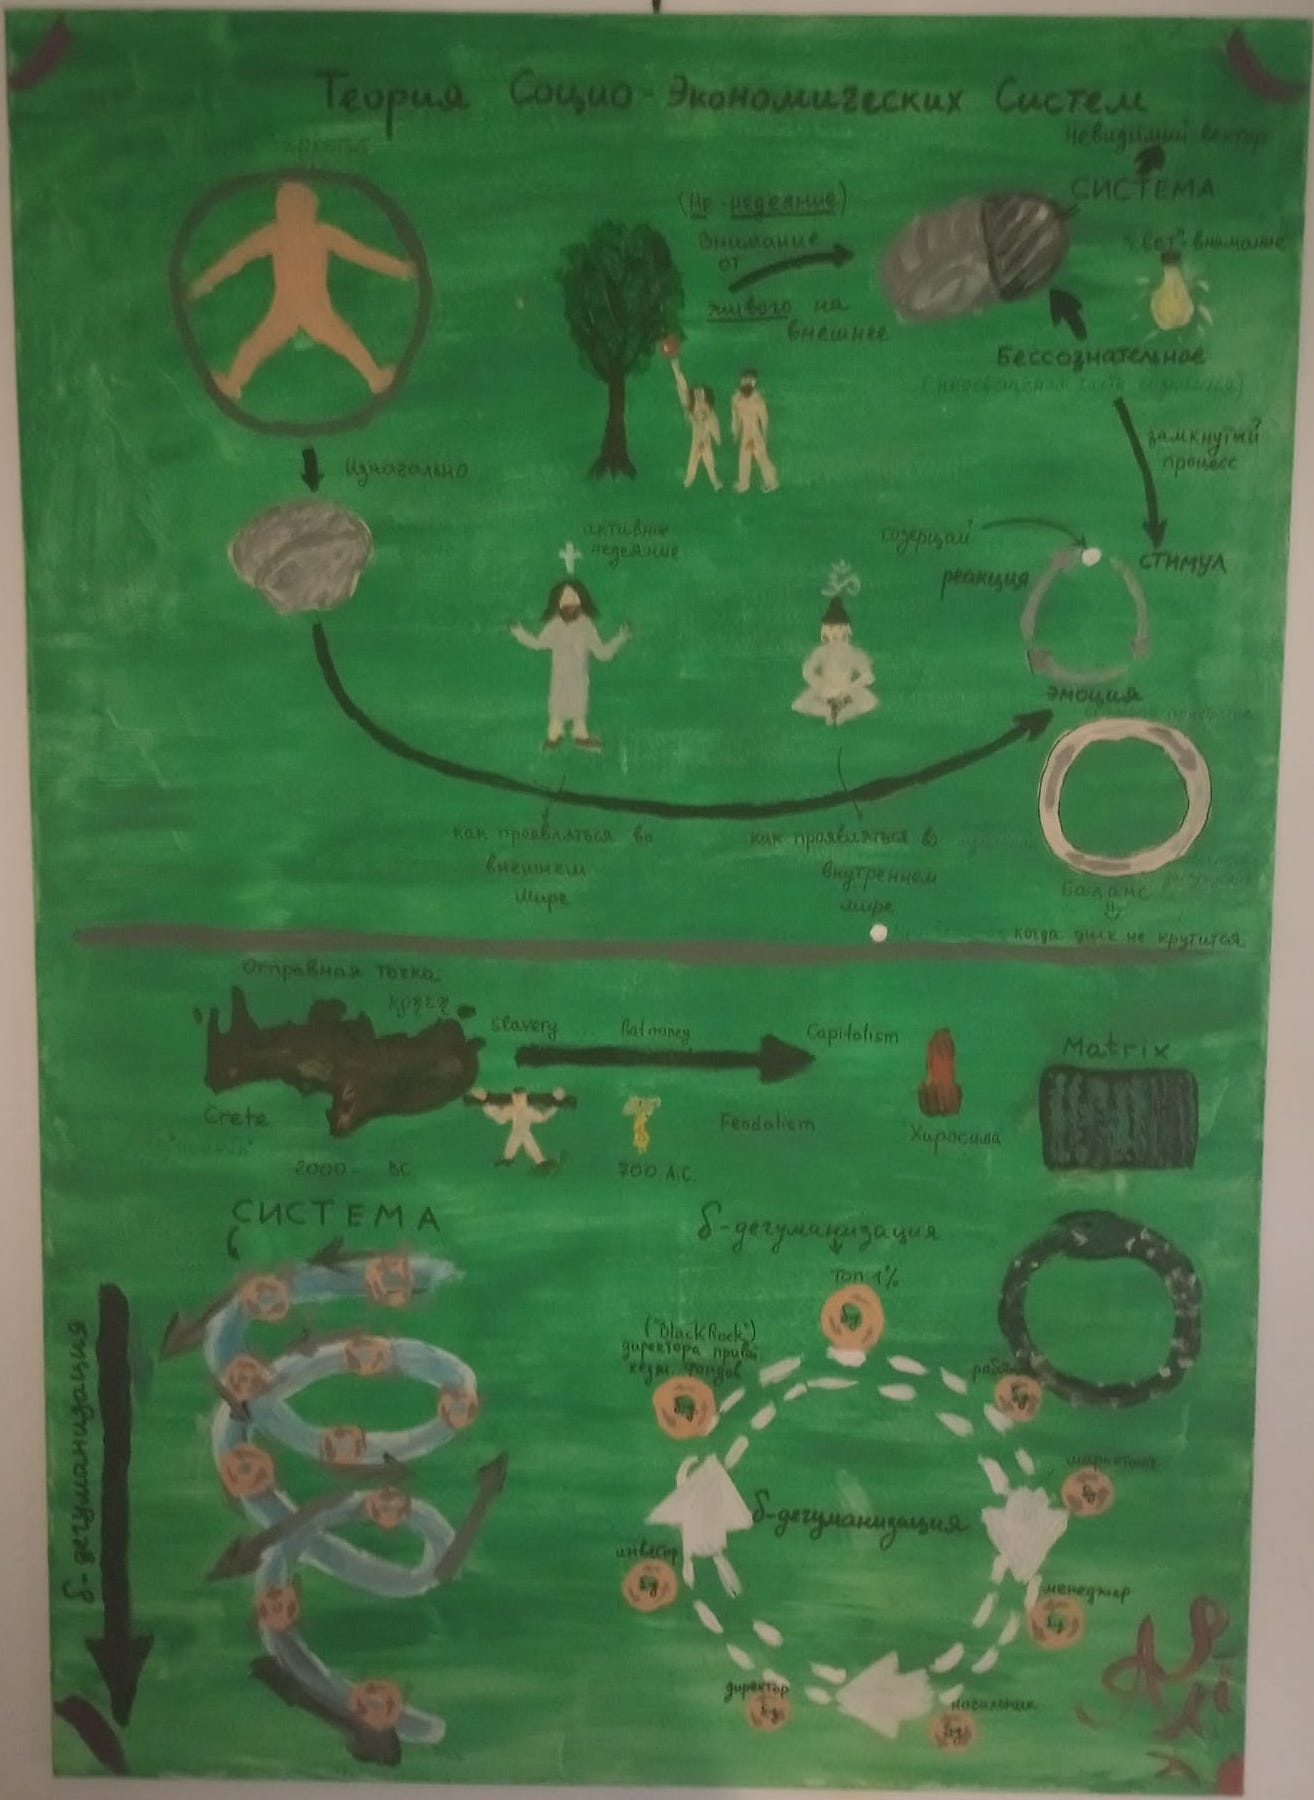
\includegraphics[width=0.8\textwidth]{fig/theory.jpeg}
    \caption{Theory meets practice: The bridge from conceptual framework to empirical validation}
    \label{fig:theory_practice}
\end{figure}

\section{Counterarguments and Responses}

We address the strongest objections to S.V.E.'s framework.

\subsection{``This is overly simplistic / reductionist''}

\textit{Objection:} Reality is too complex to be captured by a single framework like \SES{} or explained by a pattern like SYSTEM. You're reducing multifaceted phenomena to abstract models.

\textit{Response:} All models are simplifications---that's what makes them useful. The question is whether the simplification captures essential dynamics while discarding noise.

S.V.E. is not claiming to explain \textit{everything}. It's providing a \textit{lens} that reveals patterns invisible in conventional analyses. Like Newtonian mechanics: not the ultimate truth, but a powerful tool for certain scales and questions.

Moreover, \SES{} is explicitly multi-dimensional, integrating economic, social, psychological, spiritual, and environmental factors. That's the opposite of reductionism---it's synthesis across domains usually studied in isolation.

\subsection{``Consciousness is too vague / unmeasurable''}

\textit{Objection:} Consciousness is subjective and fuzzy. You can't build rigorous theory on such soft foundations.

\textit{Response:} Consciousness is no more vague than concepts like ``utility'' (economics) or ``fitness'' (biology), both of which ground successful scientific frameworks.

We define consciousness operationally:
\begin{itemize}
    \item \textit{Awareness:} What \% of relevant information is perceived vs. filtered
    \item \textit{Integration:} Degree of internal coherence vs. fragmentation
    \item \textit{Reflectivity:} Capacity to examine own thinking and assumptions
    \item \textit{Agency:} Ability to act from choice vs. automatic pattern
\end{itemize}

Each can be measured through combination of self-report, behavioral tests, and neurological correlates. Not perfect, but sufficient for scientific progress.

Furthermore, the measurability objection is weakening as neuroscience advances. We can now literally watch consciousness in action via fMRI, EEG, and other tools.

\subsection{``You're just describing capitalism---not discovering something new''}

\textit{Objection:} Marx, Veblen, Galbraith, and others described exploitative dynamics long ago. You're repackaging old critiques with new jargon.

\textit{Response:} Partially true and not a problem. We stand on their shoulders and acknowledge it explicitly.

What's new in S.V.E.:
\begin{enumerate}
    \item \textbf{Integration across domains:} Connecting economic analysis with consciousness theory, systems science, and spiritual wisdom in unified framework
    \item \textbf{Mathematical formalization:} Providing rigorous models (geodesics, attractor dynamics, feedback equations) rather than only qualitative descriptions
    \item \textbf{Actionable solutions:} Not just critique but practical alternatives (PEMY, consciousness protocols, transition strategies)
    \item \textbf{Verification protocols:} Making claims falsifiable and testable
    \item \textbf{Multi-level intervention:} Individual + systemic change, not one or the other
\end{enumerate}

If S.V.E. were merely repeating past work, it would be unnecessary. But synthesis itself creates value---seeing connections invisible when domains are studied separately.

\subsection{``The historical analysis is cherry-picked / oversimplified''}

\textit{Objection:} History is messy. You present a neat narrative of ``Fall'' but reality had ups and downs, progress and regress, across different cultures and eras. Your grand narrative is cherry-picking evidence that fits.

\textit{Response:} Fair criticism partially. History indeed is non-linear and culture-specific.

But: We're identifying \textit{patterns} not writing comprehensive history. The claim is not that every society declined monotonically, but that certain structural patterns (wealth concentration, institutionalized extraction, consciousness suppression) tend to emerge and self-reinforce.

Exceptions exist (Minoan Crete, some indigenous societies) and are important---they prove alternatives are possible. But the overall trajectory of large-scale civilizations over past 5000 years does show increasing complexity, hierarchy, and (until recently) material wealth, alongside decreasing autonomy, meaning, and connection for most people.

Open question: Was this trade-off necessary, or could we have achieved material progress without consciousness regression? S.V.E. argues the latter---PEMY is attempt to prove it.

\subsection{``This requires too much change---not realistic''}

\textit{Objection:} Your vision would require fundamental restructuring of economics, culture, institutions, and psychology. That's not going to happen. People are too invested in current systems.

\textit{Response:} Two responses:

\textbf{First:} ``Not realistic'' according to what baseline? If baseline is ``continuing current path'', then yes, transformation seems unlikely. But current path is \textit{unsustainable}---it leads to collapse. So the choice is not ``change vs. stability'' but ``conscious change vs. catastrophic change''.

\textbf{Second:} History shows that seemingly impossible transformations can happen within decades:
\begin{itemize}
    \item Abolition of slavery (went from normal to illegal in ~80 years)
    \item Women's suffrage (from unthinkable to universal in ~100 years)
    \item Civil rights (major legal changes in ~20 years of concentrated effort)
    \item Internet adoption (from novelty to ubiquitous in ~25 years)
    \item Renewable energy (from niche to cost-competitive in ~20 years)
\end{itemize}

When consciousness reaches critical mass, rapid phase transitions become possible. Not guaranteed, but not impossible either.

\subsection{``You're being elitist / talking down to people''}

\textit{Objection:} Your framing of ``unconsciousness'' and ``dehumanization'' implies you've achieved some superior state and everyone else is asleep. That's arrogant.

\textit{Response:} If it comes across that way, we've communicated poorly.

S.V.E. is explicitly \textit{not} claiming superior consciousness by authors. We're subject to the same patterns and conditioning as everyone else. The only difference: we've made SYSTEM-analysis our focus, so we've spent time mapping its structure.

The ``unconscious'' label is descriptive, not pejorative. It means: running automated patterns without awareness of running them. We \textit{all} do this constantly. Consciousness development is about gradually seeing more patterns as they run, not achieving some perfect enlightened state.

Moreover, S.V.E. emphasizes that SYSTEM is \textit{systemic}---no one is to blame individually. The wealthy are often as trapped (in different way) as the poor. We're all caught in inherited structures. The task is escaping together, not blaming anyone.

\subsection{``What about human nature? Aren't we inherently selfish/violent?''}

\textit{Objection:} Your vision assumes humans can be cooperative and conscious. But human nature is competitive, tribal, and often violent. History is full of war and exploitation. Maybe SYSTEM reflects our nature, not distorts it.

\textit{Response:} The ``human nature'' argument is double-edged. Humans are capable of both cooperation and competition, altruism and selfishness, wisdom and foolishness. Which aspect dominates depends on \textit{context}---the structures we inhabit.

Evidence:
\begin{itemize}
    \item Hunter-gatherer societies: Mostly egalitarian, low violence, high cooperation (for 95\% of human history)
    \item Children: Naturally empathetic and fair-minded before conditioning
    \item Crisis situations: People often help each other (not loot) contrary to expectation
    \item Cooperatives: Prove that people can work together without coercion when structure supports it
\end{itemize}

``Human nature'' is not fixed essence but phenotypic plasticity---we adapt to environments. SYSTEM creates environments that bring out competitive, fearful, selfish aspects. Alternative structures can bring out cooperative, generous, conscious aspects.

The question is not ``what is human nature?'' but ``what context do we want to create?''

\begin{figure}[H]
    \centering
    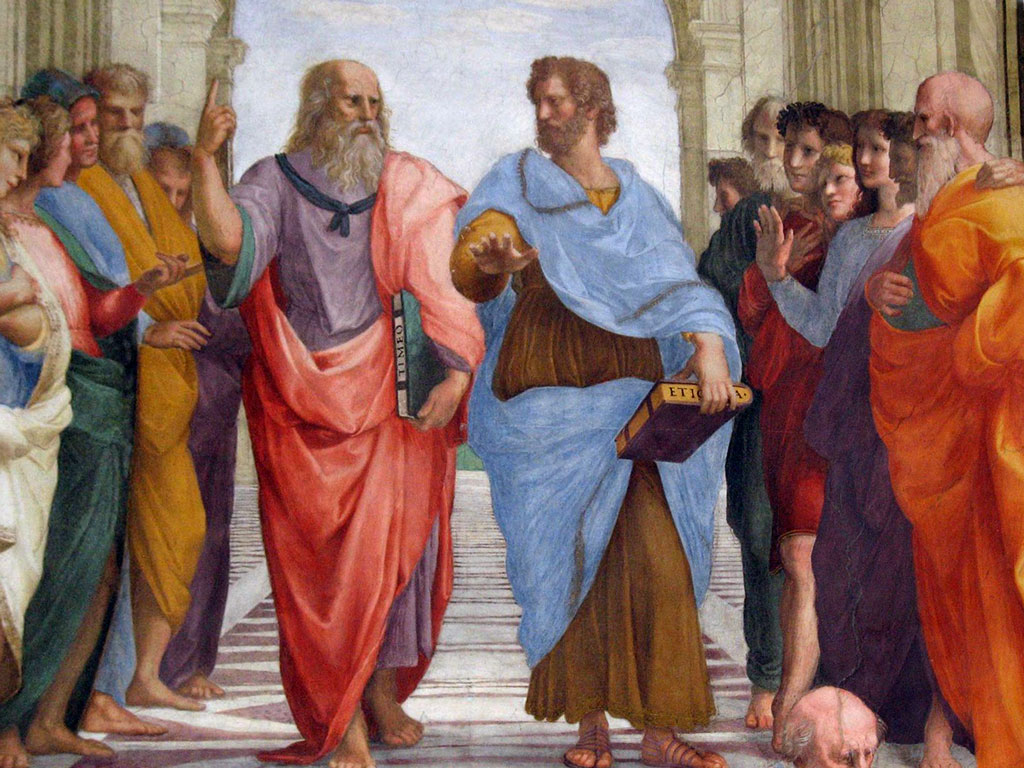
\includegraphics[width=0.7\textwidth]{fig/plato_socrates.jpeg}
    \caption{Plato and Socrates: Ancient wisdom on human nature and social structures}
    \label{fig:plato_socrates}
\end{figure}

As Plato explored in The Republic \citep{plato_republic}: the question is not just ``what is justice?'' but ``what social structure cultivates justice in individuals?'' Structure and individual co-evolve.

\section{Practical Action Steps: What You Can Do}

Theory is valuable, but action is necessary. Here are concrete steps at various levels.

\subsection{Personal Level (Start Immediately)}

\begin{enumerate}
    \item \textbf{Begin consciousness practices:}
    \begin{itemize}
        \item Implement SIP (Structured Introspection Protocol) daily for 30 days
        \item Notice one unconscious pattern per week and experiment with changing it
        \item Reclaim attention: one week digital detox
    \end{itemize}
    
    \item \textbf{Audit your participation in SYSTEM:}
    \begin{itemize}
        \item Where does your money go? (Bank, investments, purchases)
        \item What do you consume without conscious choice?
        \item What do you do because ``everyone does it''?
    \end{itemize}
    
    \item \textbf{Develop antifragility:}
    \begin{itemize}
        \item Learn practical skills (cooking, repair, first aid, gardening)
        \item Reduce debt where possible
        \item Build local relationships and community
    \end{itemize}
    
    \item \textbf{Study systems thinking:}
    \begin{itemize}
        \item Read widely: Economics, psychology, systems theory, history
        \item Practice seeing patterns across domains
        \item Engage with S.V.E. other papers in series
    \end{itemize}
\end{enumerate}

\subsection{Interpersonal Level (Within 3 Months)}

\begin{enumerate}
    \item \textbf{Start conversations:}
    \begin{itemize}
        \item Share S.V.E. ideas with 5-10 people
        \item Not to convert, but to test ideas and learn from objections
        \item Form reading/discussion group around consciousness and systems
    \end{itemize}
    
    \item \textbf{Model alternatives:}
    \begin{itemize}
        \item Make one major life decision using conscious values (not default scripts)
        \item Share the reasoning publicly (blog, social media, conversations)
        \item Inspire others by example
    \end{itemize}
    
    \item \textbf{Support existing alternatives:}
    \begin{itemize}
        \item Buy from cooperatives and B Corps when possible
        \item Bank with credit unions not mega-banks
        \item Patronize local/sustainable businesses
    \end{itemize}
\end{enumerate}

\subsection{Organizational Level (Within 1 Year)}

\begin{enumerate}
    \item \textbf{If you work somewhere:}
    \begin{itemize}
        \item Propose transparency increases (open salaries, decision processes)
        \item Advocate for stakeholder representation
        \item Start conversation about converting to B Corp or cooperative structure
    \end{itemize}
    
    \item \textbf{If you're starting something:}
    \begin{itemize}
        \item Design it as PEMY from day one
        \item Document the process and share learnings
        \item Connect with PEMY network (to be created)
    \end{itemize}
    
    \item \textbf{If you have capital:}
    \begin{itemize}
        \item Invest in PEMY-type entities
        \item Provide patient capital (long-term, stakeholder-oriented)
        \item Support platform cooperatives and B Corps
    \end{itemize}
\end{enumerate}

\subsection{Community Level (Ongoing)}

\begin{enumerate}
    \item \textbf{Build mutual aid networks:}
    \begin{itemize}
        \item Time banks, skill-sharing, resource pooling
        \item Support systems outside market/government
        \item Practice cooperation at small scale
    \end{itemize}
    
    \item \textbf{Participate in local governance:}
    \begin{itemize}
        \item Attend city council, school board meetings
        \item Advocate for transparency, participation, long-term thinking
        \item Run for local office or support aligned candidates
    \end{itemize}
    
    \item \textbf{Create educational spaces:}
    \begin{itemize}
        \item Workshops on consciousness practices
        \item Discussion groups on systems and alternatives
        \item Youth programs teaching critical thinking and EBP
    \end{itemize}
\end{enumerate}

\subsection{Cultural Level (Continuous)}

\begin{enumerate}
    \item \textbf{Shift narratives:}
    \begin{itemize}
        \item Write, speak, create art about alternative visions
        \item Challenge SYSTEM assumptions in everyday conversations
        \item Celebrate examples of cooperation and consciousness
    \end{itemize}
    
    \item \textbf{Support transformative media:}
    \begin{itemize}
        \item Fund/promote content exploring consciousness and systems
        \item Create documentaries, books, podcasts on these themes
        \item Use social media to amplify alternative voices
    \end{itemize}
    
    \item \textbf{Develop collective intelligence:}
    \begin{itemize}
        \item Contribute to Verifiable Knowledge Base (S.V.E. project)
        \item Engage in Epistemological Boxing with opponents
        \item Refine and evolve S.V.E. frameworks collaboratively
    \end{itemize}
\end{enumerate}

\subsection{The 80/20 Recommendation}

If you only do three things:

\begin{enumerate}
    \item \textbf{Develop your own consciousness} (personal practices, minimum 15 min/day)
    \item \textbf{Build real community} (local, embodied relationships with mutual support)
    \item \textbf{Participate in or create one PEMY-type entity} (prove alternatives work)
\end{enumerate}

These three have multiplier effects. Conscious individuals create culture. Strong communities resist SYSTEM capture. Functional alternatives spread by demonstration.

\section{Conclusion: The Choice Ahead}

We stand at a bifurcation point. Humanity can continue on current trajectory---which leads to collapse, whether catastrophic or gradual, within this century. Or we can consciously choose transformation---which requires facing uncomfortable truths, letting go of inherited patterns, and building something fundamentally different.

\subsection{The Inyan-Uber Synthesis}

\begin{figure}[H]
    \centering
    \includegraphics[width=0.75\textwidth]{fig/in_yan_uber_type_1_type_2.png}
    \caption{The Yin-Yang of socioeconomic evolution: Integrating opposing forces into higher synthesis}
    \label{fig:yinyang_synthesis}
\end{figure}

Think of current situation as tension between opposing forces:
\begin{itemize}
    \item \textbf{Yang (Type 1):} Efficiency, competition, growth, innovation, individual achievement
    \item \textbf{Yin (Type 2):} Sustainability, cooperation, stability, wisdom, collective flourishing
\end{itemize}

Neither alone is sufficient. Pure competition leads to winner-take-all dystopia. Pure cooperation without excellence leads to stagnation. We need \textbf{synthesis}: competitive innovation within cooperative frameworks, individual achievement serving collective good.

PEMY attempts this synthesis: retaining market dynamics and innovation incentives while embedding them in structures that prevent extraction and dehumanization.

\subsection{Artemisia: Symbol of Healing}

\begin{figure}[H]
    \centering
    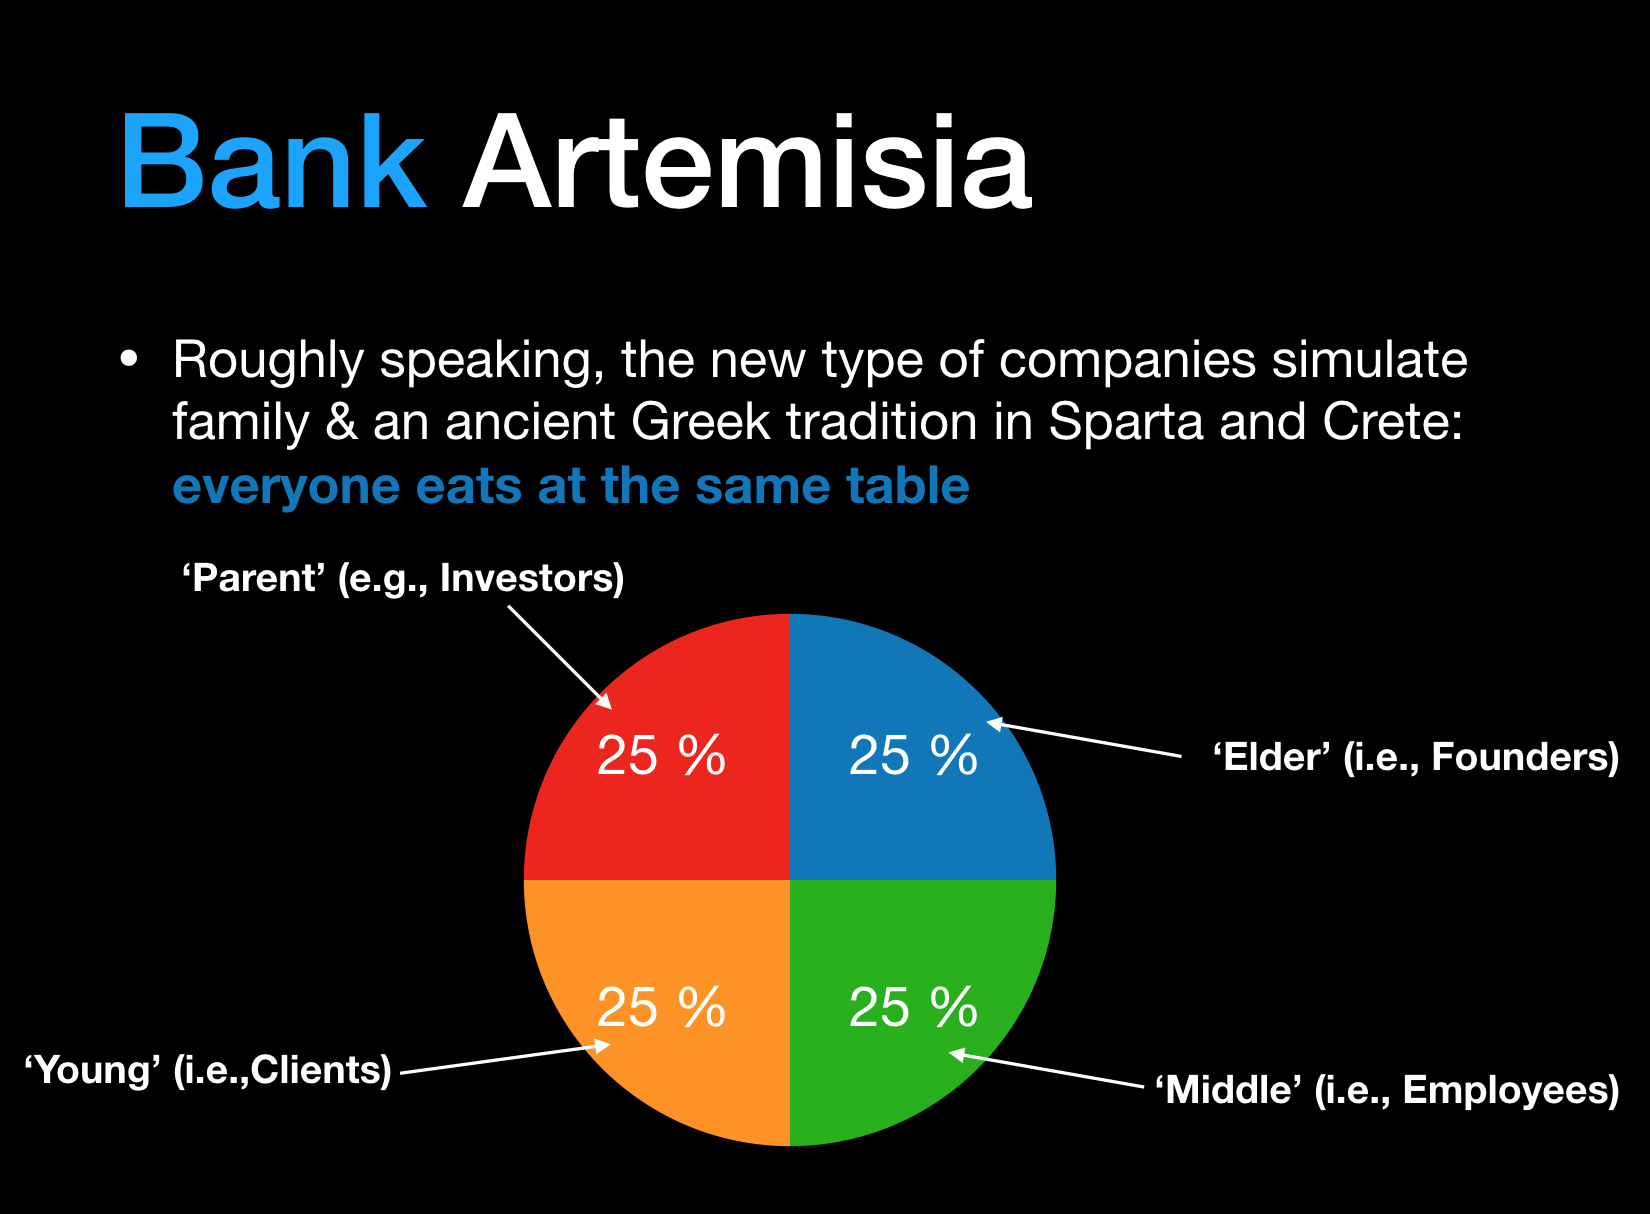
\includegraphics[width=0.6\textwidth]{fig/bank_artemisia_illustration.png}
    \caption{Artemisia: The healing herb as metaphor for social transformation}
    \label{fig:artemisia}
\end{figure}

The artemisia plant has been used medicinally for millennia---bitter but healing. It's fitting metaphor for transformation:

The truth about SYSTEM is bitter. Facing our collective unconsciousness is uncomfortable. Dismantling inherited structures feels threatening. But this bitterness is healing.

Like medicine that tastes bad but cures disease, confronting SYSTEM and choosing conscious evolution may be difficult but is ultimately what allows humanity to thrive rather than merely survive (or collapse).

\subsection{The Final Question}

Every person reading this must answer:

\begin{center}
\textbf{Will I participate consciously in transformation,\\
or unconsciously in continuation of patterns that lead to suffering?}
\end{center}

This is not moral judgment---no one is bad for choosing unconsciousness. But it \textit{is} a choice with consequences. And increasingly, individual choices aggregate into collective trajectory.

Think of it like voting---except the election is continuous and the outcome is humanity's future. Every decision you make is a vote: For consciousness or pattern. For regeneration or extraction. For truth or delusion. For life or entropy.

\subsection{The Practical Hope}

This paper may seem heavy---diagnoses are often grim. But there is genuine hope:

\begin{itemize}
    \item \textbf{Alternatives exist:} PEMY and similar models are proven workable
    \item \textbf{Consciousness can develop:} Practices work, transformation is possible
    \item \textbf{Small groups can catalyze large change:} Historical precedents exist
    \item \textbf{Technology can serve awakening:} Not all digital tools are extractive
    \item \textbf{Younger generations are ready:} Many already reject SYSTEM's premises
\end{itemize}

The future is not determined. It's being created now, by choices made individually and collectively. The question is whether those choices will be conscious.

\subsection{Invitation}

S.V.E. is not finished work but ongoing project. We invite:

\begin{itemize}
    \item \textbf{Critique:} Find flaws, challenge assumptions, improve models
    \item \textbf{Contribution:} Add your insights, expertise, and perspectives
    \item \textbf{Implementation:} Try these ideas in real contexts and report results
    \item \textbf{Collaboration:} Join in building Verifiable Knowledge Base and PEMY network
    \item \textbf{Translation:} Bring these ideas to other languages and cultures
\end{itemize}

No single person or paper will solve humanity's challenges. But collective intelligence, grounded in consciousness and structured by rigorous method, can navigate complexity that defeats individuals and institutions.

\subsection{Closing Meditation}

Imagine humanity 100 years from now. Two possible futures:

\textbf{Future A (Unconscious Continuation):}
Survivors living in climate-devastated world, under authoritarian control, with most beauty and diversity lost, asking ``how did we let this happen?''

\textbf{Future B (Conscious Evolution):}
Thriving communities, restored ecosystems, meaningful work, genuine connection, diverse expressions of human potential, looking back with gratitude at the generation that chose transformation.

Which future do we create? The answer lies not in grand political movements (though those help) but in \textbf{daily choices}:

\begin{itemize}
    \item Do you consume unconsciously or choose consciously?
    \item Do you compete extractively or cooperate generatively?
    \item Do you follow inherited scripts or write new ones?
    \item Do you participate in dehumanizing systems or build humanizing alternatives?
    \item Do you defend patterns out of fear or embrace growth toward love?
\end{itemize}

These are not abstractions. They're the actual shape of the work.

\vspace{1cm}

\begin{center}
\textit{The future is not inevitable.}\\
\textit{It is chosen.}\\
\textit{Choose consciously.}\\
\textit{Choose together.}\\
\textit{Choose love over fear, truth over comfort, life over entropy.}\\[0.5cm]

\textbf{С Богом! --- With God!}\\
\textbf{С Любовью! --- With Love!}\\
\textbf{We can do this.}
\end{center}

% ==================== APPENDICES ====================
\appendix

\subsection*{Extension: Vecheism and the Organizational Constructor}

Beyond its economic dimension, PEMY can be operationalized through a meta-organizational framework tentatively termed the \textbf{Organizational Constructor} or \textbf{Vecheism}.  
It proposes the creation of flexible, adaptive socio-economic systems with continuous feedback loops---a living synthesis of ancient civic self-governance (\textit{Veche}, \textit{Syssitia}) and modern digital coordination (DAO, doola).

\begin{quote}
``Building flexible and adaptive systems of interaction of any complexity, with continuous feedback.'' — A. Kovnatsky
\end{quote}

\paragraph{Core Principles.}
\begin{enumerate}[noitemsep,topsep=0pt]
    \item \textbf{Justice, Brotherhood, and Family Values:} every participant benefits from shared resources, countering the ``1\% extraction'' dynamic.
    \item \textbf{Equal Participatory Shares:} governance distributed among four stakeholder groups---State, Owners, Workers, and Citizens---each holding 25\% share and weighted voting rights.
    \item \textbf{Light Reprivatization:} partial nationalization of enterprises exploiting common goods, ensuring lifelong security for owners (25\% retained share or hereditary compensation).
    \item \textbf{Digital Governance:} dividends, voting, and resource allocation processed via national digital services (\textit{e.g., GosUslugi}), guaranteeing transparency.
    \item \textbf{Constructive Dialogue Table:} equal representation of social strata, promoting project-based collaboration and conflict resolution.
\end{enumerate}

\paragraph{Implementation Architecture.}
\begin{itemize}[noitemsep,topsep=0pt]
    \item \textbf{Hybrid Governance:} real meetings complemented by blockchain-based assemblies; instantaneous creation and management of legal entities (“one-click” DAO–LLC hybrids).
    \item \textbf{Continuous Feedback:} real-time monitoring of performance, motivation, and systemic balance with semi-automatic rebalancing and human override.
    \item \textbf{Transparent Ledgers:} dual-layer (open + closed) blockchain infrastructure for public accountability and national security.
\end{itemize}

\paragraph{Strategic Outcomes.}
\begin{itemize}[noitemsep,topsep=0pt]
    \item Strengthened resilience and self-regulation of national and corporate ecosystems.
    \item Reduction of social tension via participatory dividends.
    \item Attraction and retention of top talent through purpose-driven ownership.
    \item A global alternative to extractive capitalism: “centralized decentralization” for collective prosperity.
\end{itemize}

\paragraph{Relation to PEMY.}
Vecheism operationalizes PEMY's principles—ethical participation, adaptive fairness, and systemic feedback—into a technological and institutional framework. It serves as a socio-technical layer bridging S.V.E. governance theory with practical civic infrastructure.

\begin{figure}[h]
\centering
\includegraphics[width=0.85\linewidth]{fig/vecheism_structure.png}
\caption{Conceptual model of the Vecheism-based Organizational Constructor integrating PEMY governance and digital feedback mechanisms.}
\label{fig:vecheism}
\end{figure}


\section{Minoan Crete: A Counter-Example to Violent Inevitability}
\label{app:minoan}

The Minoan civilization (ca. 3000-1100 BCE) on Crete presents fascinating counter-evidence to claims that hierarchy and violence are inevitable in complex societies.

\textbf{Key Features:}
\begin{itemize}
    \item Absence of fortifications (unlike contemporary civilizations)
    \item Art emphasizing nature, play, celebration (not warfare or domination)
    \item Evidence of relatively flat social hierarchy
    \item Women in prominent religious and possibly political roles
    \item Extensive trade networks (cooperation rather than conquest)
    \item High cultural achievement (architecture, art, engineering)
\end{itemize}

\textbf{Implications:}
If Minoans could build complex civilization without militarization and extreme hierarchy for nearly 2000 years, then such features are not \textit{necessary} for complexity---they're \textit{choices}, even if often unconscious ones.

Their eventual decline (possibly from volcanic eruption and subsequent conquest) doesn't negate this lesson. It shows that non-violent societies can be vulnerable to violent ones---which is argument for transforming \textit{all} societies, not abandoning the attempt.

\section{Against the Trolley Problem: A Systems-Engineering Critique}
\label{subsec:trolley}

The famous trolley problem (``pull lever to kill one person instead of five?'') is often treated as fundamental ethical dilemma. S.V.E. argues it's actually a \textbf{distraction from systems thinking}.

\textbf{Problems with Trolley Framing:}
\begin{enumerate}
    \item \textbf{Normalizes ``choice of victim'':} Accepts that someone must die, focuses on optimization rather than prevention
    
    \item \textbf{Ignores root causes:} Who built the trolley? Who maintained the tracks? Why are people tied to rails? These are the real questions.
    
    \item \textbf{Individualistic framing:} One person making choice vs. systemic responsibility
    
    \item \textbf{Time-pressured decision:} Eliminates possibility of creative solutions (stop trolley, warn people, coordinate rescue)
    
    \item \textbf{Training for compliance:} Gets people comfortable with ``choosing the lesser evil'' rather than refusing false dilemmas
\end{enumerate}

\textbf{S.V.E. Response:}
Real-world ethical challenges are almost never trolley problems. They're systems problems: How do we design societies where trolley situations don't arise? How do we create feedback loops that surface problems before they become crises?

The right answer to trolley problem is: \textbf{Reject the premises. Redesign the system.}

This is not evasion---it's the only response that actually reduces suffering long-term. Pulling the lever (either way) accepts the framing and ensures similar situations recur. Fixing the system prevents them entirely.

\section{What Makes S.V.E. Unique?}
\label{subsec:sve_unique}

Many frameworks attempt to address social/economic/spiritual challenges. What distinguishes S.V.E.?

\begin{enumerate}
    \item \textbf{Operationalized Epistemology:}
    \\
    Not just theory of knowledge but \textit{protocols} (EBP, SIP) executable by individuals and institutions
    
    \item \textbf{Mathematics of Meaning:}
    \\
    Rigorous formalization of consciousness and ethics using differential geometry, not just qualitative descriptions
    
    \item \textbf{Institutional Antifragility:}
    \\
    Design principles for structures that improve through challenge rather than breaking (limited-by-design + adversarial verification)
    
    \item \textbf{Unified Epistemology \& Ethics:}
    \\
    Geodesic framework unifies ``true'' and ``good''---they point same direction in consciousness space
    
    \item \textbf{Falsifiable Predictions:}
    \\
    Unlike many philosophical/spiritual frameworks, S.V.E. makes testable claims about reality
    
    \item \textbf{Individual + Systemic:}
    \\
    Addresses both personal consciousness development and structural transformation (most approaches do one or the other)
    
    \item \textbf{Practical Implementation:}
    \\
    Not just critique but concrete alternatives (PEMY, protocols, transition strategies)
\end{enumerate}

\section{Acknowledgments}

This work synthesizes insights from:

\begin{itemize}
    \item \textbf{Philosophical Wisdom:} Plato, Socrates, Christ, Buddha, Marcus Aurelius, Lao Tzu, Spinoza, Kant, and many others across traditions
    
    \item \textbf{Economic Analysis:} Adam Smith \citep{smith1776wealth}, Marx, Veblen, Galbraith, Piketty \citep{piketty2014capital}
    
    \item \textbf{Psychological Insight:} Jung \citep{jung1969collective}, Freud, Kahneman \citep{kahneman2011thinking}, depth psychology traditions
    
    \item \textbf{Systems Science:} Complexity theory, cybernetics, network science, resilience research
    
    \item \textbf{Strategic Thought:} Pereslegin \citep{pereslegin2005summa}, Sun Tzu \citep{suntzu_artofwar}, Machiavelli \citep{machiavelli1532prince}
    
    \item \textbf{Contemporary Critique:} Chomsky, Taleb \citep{taleb2012antifragile}, critical theorists, post-colonial scholars
    
    \item \textbf{AI-Assisted Synthesis:} Claude by Anthropic (for modeling, analysis, synthesis)
    
    \item \textbf{Lived Experience:} Humanity under various \SES{} structures across history
    
    \item \textbf{Collective Consciousness:} The ultimate author
\end{itemize}

\textbf{Special Gratitude:}
\begin{itemize}
    \item To philosophical ancestors for lighting the path
    \item To psychological pioneers for mapping the unconscious
    \item To economic thinkers for revealing system dynamics
    \item To strategic theorists for understanding power and change
    \item To S.V.E. community for engagement, critique, and refinement over years of dialogue
    \item To all humans striving toward awareness and love---this is our collective work
\end{itemize}

\vspace{1em}

\textbf{To the Reader:}

Thank you for engaging with these ideas. Your attention, critical thinking, and potential action are themselves acts of resistance against SYSTEM's unconscious pull. The fact that you've read this far suggests you're already choosing consciousness. May that choice continue to deepen.

\section{Contact and Collaboration}

S.V.E. is an open project welcoming:

\begin{itemize}
    \item \textbf{Critiques and counterarguments} (via Epistemological Boxing if desired)
    \item \textbf{Collaborative refinement} of models and frameworks
    \item \textbf{Implementations} of PEMY or other S.V.E. tools in real-world contexts
    \item \textbf{Contributions} to the Verifiable Knowledge Base
    \item \textbf{Translations} into other languages
    \item \textbf{Research collaborations} and empirical testing
    \item \textbf{Educational initiatives} using S.V.E. frameworks
    \item \textbf{Artistic expressions} of these ideas (film, music, visual art, literature)
\end{itemize}

\textit{[Contact information and project links would be included here in a published version]}

% ==================== BIBLIOGRAPHY ====================
\bibliographystyle{plainnat}
\bibliography{\jobname}

\end{document}